\documentclass[a4paper,10pt,oneside]{book}
\usepackage{titling}

\usepackage[utf8]{inputenc}
\usepackage{amsmath}
\usepackage{graphicx}
\usepackage{tabularx}
\usepackage{subcaption}
\usepackage[]{caption}

\usepackage[a4paper, total={6in, 8in}]{geometry}
\usepackage[dvipsnames]{xcolor}
\usepackage{tcolorbox}
\usepackage[colorlinks=true, urlcolor=BurntOrange]{hyperref}
\usepackage{physics}

\usepackage{nicefrac}
\usepackage{enumitem}
\graphicspath{{figs/}}

\setlength{\parskip}{\baselineskip}%
\setlength\parindent{0pt}

\usepackage{color, colortbl}
\usepackage{bm}
\definecolor{Gray}{gray}{0.9}

\usepackage{pdfpages}

\newcolumntype{L}[1]{>{\raggedright\arraybackslash}p{#1}}
\newcolumntype{C}[1]{>{\centering\arraybackslash}p{#1}}
\newcolumntype{R}[1]{>{\raggedleft\arraybackslash}p{#1}}



% \newtcolorbox{imp}{colback=orange!5!white,colframe=orange!75!black,fonttitle=\bfseries,title=Important}

% \newtcolorbox{question}{colback=red!5!white,colframe=red!75!black,fonttitle=\bfseries,title=Question}

\newtcolorbox{imp}{colback=orange!5!white,colframe=orange!75!black,fonttitle=\bfseries}

\newtcolorbox{question}{colback=red!5!white,colframe=red!75!black,fonttitle=\bfseries}

\newtcolorbox{tip}{colback=green!5!white,colframe=green!35!black,fonttitle=\bfseries,title=Tip}


%% [[ DEFINING `POLYTECHNIQUE' COLOURS
\definecolor{Blue}{RGB}{0,59,92}
\definecolor{Grey}{RGB}{74,73,72}
\definecolor{Red}{RGB}{247,38,22}
\definecolor{DarkRed}{RGB}{197,26,27}
\definecolor{Yellow}{RGB}{223,176,0}
\definecolor{White}{RGB}{255,255,255}
%% END POLYTECHNIQUE COLORS]]


\usepackage{color,soul}
\usepackage{tikz}
\setulcolor{Red}
\setul{}{2pt}

\usepackage{chngcntr} 
\usepackage{fancyhdr}
\counterwithin{section}{chapter}
\makeatletter
\@addtoreset{chapter}{part}
\makeatother 
\renewcommand{\thepart}{\Roman{part}}

\begin{document}

\title{\vspace{8cm}\LARGE \textcolor{Blue}{\textsc{PHY102:\\An Introduction to Physics through Experiments}}}
%\author{\textsc{Philip Cherian}}
\date{}


\maketitle



\tikz[remember picture,overlay]\node[shift={(,)},opacity=0.4] at (current page.south east) {
\includegraphics[width=17.5cm]{logo}};
%\tikz[remember picture,overlay]\node[shift={(2.25cm,-2.75cm)},opacity=1] at (current page.north west) {
\includegraphics[width=3cm]{logo.png}};

\thispagestyle{empty}
\newpage

\frontmatter
{
\setcounter{tocdepth}{1}
\hypersetup{linkcolor=black}
\tableofcontents
}

% % \clearpage
% % \setcounter{page}{1}
% \mainmatter

% \vbox{
% \textcolor{Blue}{\part{Introductory Sessions}}
% \tikz[remember picture,overlay]\node[shift={(-1,1)},opacity=0.6] at (current page.south east) {
\includegraphics[width=17.5cm]{logo}};
% }

% \renewcommand{\chaptername}{Session}

% \chapter{Data Collection, Recording, and Interpretation}

\section{Objectives}

\begin{enumerate}
    \item To understand basic data collection, representation, and interpretation using a simple pendulum.
\end{enumerate}

\section{Introduction}

In this preliminary experiment you will use a simple and familiar system, the simple pendulum, to understand measurement, data collection, and elementary data interpretation. In this experiment, as in many others that you will do in this lab, you will observe a system that is well understood. You will often want to know how a certain property of the system changes when one of the parameters of the system is changed. For example, in this experiment, you might ask: How does the the time period vary with the mass of the bob? How does the time period vary with the length of the pendulum? Alternatively, you may want to set up an experiment that leads to a particular value for a certain property. For example, you may ask: How long does the pendulum need to be for its period to be 1 second?

\section{Data Collection}

Data collection is the observing and recording of data using instruments. You will record data in a \textit{log book} -- preferably a thick and sturdy hard-covered notebook that lasts the entire semester (or, if you intend to major in physics, perhaps all your years at Ashoka).

\subsection{Recording Raw Data}

\subsubsection{Raw Data vs Processed Data}

Raw data is what you see on your measuring instruments. Recording it is the first important step in experimental physics. Raw data is distinct from processed data, and it is important never to forget the difference between them. For example, if you measure the time for 10 oscillations of a pendulum, it is the time for 10 oscillations that is your raw data. You may be interested in the time period of the pendulum (i.e. the time for 1 oscillation) and to do that you will have to divide the measurement you have made by 10; the moment you do this, you have performed an operation on it, i.e.\ you have processed your data. 
\begin{imp}
In experimental physics, you must never, under any circumstances, process your data on the fly before recording it: what you must record, first and foremost, is what you see on your measuring instruments. Later, you can process it and change it to any other form that suits you. 
\end{imp}

\subsubsection{Instrument Parameters}

The instrument gives you a number, which will in general have a certain dimension, with units. To make sense of the data you record, you will have to first record the units in which the numbers on the measuring device are expressed. For example, if you use a $mm$ scale to measure the length of an object, you will need to record $mm$ as your units before you take any actual readings. In a certain sense, the unit in which the number on the instrument is expressed is your first observation. (There is a reading that needs to be taken even before that -- the date on which the experiment is being done!)

\subsubsection{Tabulating Data}

In physics we are interested in patterns. One of the most compact and effective ways of recording data so that patterns can be seen easily is the table. For example, we may want to find the answer to the following question: How does the time period of a simple pendulum vary with the mass of the bob? To answer this question, we will want to take many measurements of the time period, one (or more) for each mass of bob. It follows naturally that we should align each mass with the corresponding time period, with one reading following another in vertical progression. Such an arrangement is called a table. Spend some time deciding what data table to draw before beginning your experiment: it will help you decide what data to take.

There is no strict ``right'' way to tabulate data.\footnote{However, there are several wrong ways.} An example is shown in Table (\ref{table:sampledata}).

\begin{table}[!htb]
\centering
\begin{tabular}{|C{4cm}|C{2cm}|C{2cm}|C{2cm}|C{4 cm}|}
\hline
\rowcolor{Gray}
\hline
\textbf{Mass of bob {\color{gray}(g)}} & \multicolumn{3}{|c|}{\textbf{ Time for 10 oscillations {\color{gray}(s)}}} &\textbf{Time Period {\color{gray}(s)}} \\ \hline
{} & Trial 1 & Trial 2 & Trial 3 & {} \\
\hline
{} & {} & {} & {} & {} \\
\hline
{} & {} & {} & {} & {} \\
\hline
{} & {} & {} & {} & {} \\
 \hline
\end{tabular}
\caption{Sample data table}
\label{table:sampledata}
\end{table}

In the table above, the raw data are recorded in the columns for the \textit{Mass of bob} and \textit{Time for 10 oscillations}. Note how the unit in which the measurement is taken (read from the instrument used) is noted next to the title. 

\subsubsection{Data Ethics}

It is essential that none of these readings be changed; if you wish to change a reading, strike it out gently, in such a way that it can still be seen, and write down, next to it or under it, the new reading. It is essential to have a record of all the data you have taken. Remember that this does not need to be excessively neat, only understandable to you and a trained physicist looking at your log book later, e.g. your TF or your instructor.  

If you imagine that the purpose of the experiment is to get a certain result, then you will sometimes be tempted to get rid of ``wrong'' data, but if you remember that the purpose of the experiment is to learn the methods of experimental physics, you will realise that there is no such thing as wrong data.  

This does not imply that you will always use all the data that you record. But, in general, when you discard certain data, or decide not to use it -- a process that is called ``flagging data'' -- you will have a reason for doing so. 

Before you leave the lab show your data log to your TF or course instructor and ask him or her to initial it. 

\subsubsection{``How many readings should I take?''}

This is the question we hear the most often. The answer is of course that \textbf{it depends}. It certainly depends on the experimental setup, and it depends on the different types of uncertainties present in each measurement.

While some scientific measurements are exact,\footnote{Counting the number of parents you have, for example.} others -- such as the sorts of measurements you will be doing in this lab -- are not. When we make a measurement of a quantity, we generally assume that some exact or true value exists for each, based on how we define what is being measured. We attempt to find these quantities as best we can, with the available resources, keeping in mind what we want to get eventually from the data and the effect that errors in measurement could influence our desired result (more on this in the chapter on error analysis). Appreciating this helps us understand how many readings to take. 

You will notice that you usually obtain slightly different results on making multiple measurements of the same quantity. We will deal with this in great detail in the chapter on error analysis, but for now you may imagine that these are a result of random fluctuations about the ``true'' value. One way to increase your confidence in experimental data is to repeat the same measurement many times and take the average. (We will have more to say about this later, but let us understand it intuitively first.)

For example, one way to determine the time period ($T$) of a pendulum is to measure the time for 1 oscillation. But we all understand, intuitively, that it is perhaps better to measure the time for 10 oscillations and divide by 10.  This is true. (Why this is true is not, if you think about it, so obvious -- but we will go into that later.)

But we can find the time for 10 oscillations in two different ways: (i) we can find the time for 10 oscillations in a row; (ii) we can find the time for 1 oscillations 10 times. Do these two procedures amount to the same thing? It turns out that they do not -- in the sense that the error associated with the two procedures are different. (Once again, why this is true is not obvious; let us accept it for now and understand it later.) 

Given that these two procedures for measuring $T$ are not identical, one may now ask the following question: If I want to measure the time for 100 oscillations, is it better to do that all at one go or divide it into 10 trials of 10 oscillations each? (The answer to this question is not obvious either!) 

There are all kinds of subtleties in data collection that you will slowly come to grips with. The answer to the question that is the title of this subsection is not obvious, and you will learn it slowly. 

\begin{question}
\paragraph{Question:} Can you explain why taking the time period for a 1000 oscillations may not give you an answer that is much more accurate than 100 oscillations?
\end{question}
\newpage
\section{The Experiment}

\subsection{Apparatus}

\begin{enumerate}
    \item Metallic bobs of different materials
    \item A length of string
    \item A cork with a slit
    \item A retort stand with an attached protractor
    \item A stopwatch
    \item A scale
    \item A weighing balance
\end{enumerate}

\subsection{Suggested Procedure}

\begin{question} 
\paragraph{Question:} Which are the different physical quantities in this problem that can be varied to potentially change the time period?
\end{question}

\subsubsection{Part A}

In this part of the experiment you will design a simple experiment to determine the variation of the time period with the mass of the bob.

\begin{enumerate}
    \item Begin by deciding which variables you need to fix, and which variables you will change.
    
    \item Draw out an appropriate table in your auxiliary notebooks. Mark out any important details that would help you remember what you've done when you re-read this. Remember to state not only what you have changed, but also what you have kept \textit{fixed}.
    
    \item Decide on the \textbf{number} of readings you will take. When you have arrived at a number, try to \textit{justify} it.
    
    \item Perform the necessary experiment, varying the relevant parameter. Note down your data.
    
\end{enumerate}



\subsubsection{Part B}

In this part of the experiment you will design a simple experiment to determine the variation of the time period with the length of the string from the pivot to the centre of mass of the bob.

\begin{enumerate}
    \item Begin by deciding which variables you need to fix, and which variables you will change.
    
    \item Draw out an appropriate table in your auxiliary notebooks. Mark out any important details that would help you remember what you've done when you re-read this. Remember to state not only what you have changed, but also what you have kept \textit{fixed}.
    
    \item Decide on the \textbf{number} of readings you will take. When you have arrived at a number, try to \textit{justify} it.
    
    \item Perform the necessary experiment, varying the relevant parameter. Note down your data.
    
\end{enumerate}


\subsubsection{Part C}

In this part of the experiment you will design a simple experiment to determine the variation of the time period with the angle of release of the bob.

\begin{enumerate}
    \item Begin by deciding which variables you need to fix, and which variables you will change.
    
    \item Draw out an appropriate table in your auxiliary notebooks. Mark out any important details that would help you remember what you've done when you re-read this. Remember to state not only what you have changed, but also what you have kept \textit{fixed}.
    
    \item Decide on the \textbf{number} of readings you will take. When you have arrived at a number, try to \textit{justify} it.
    
    \item Perform the necessary experiment, varying the relevant parameter. Note down your data.
    
\end{enumerate}


\paragraph{Note:} The repetition is -- of course -- intentional. We have found that students usually jump through these steps and -- as a result -- spend much of their time painstakingly collecting data that is of little or no use. It is essential that you spend some time deciding what exactly you want to collect, and how best you will represent it, before actually spending any time with the apparatus.

\begin{question}
\paragraph{Question:} In each of the above cases, which graph would be the best to plot? Why?

\paragraph{Question:} It ought to be pretty clear that $T$ should depend on the gravity of the Earth. So, ideally, we would like to vary the gravitational force as well, and see how $T$ changes. Can you think of a way in which this can be done?

\paragraph{Question:} On the basis of your experimental results (not what you learnt in school about the simple pendulum) what parameters do you find the time period $T$ depends on? How confident are you of this conclusion? What is the best way to think of the parameter(s) on which $T$ depends?

\paragraph{Question:} What would be the effect -- if any -- of changing the \textbf{shape} of the bob on the time period? Justify your answer.
\end{question}

% \begin{question}

% \end{question}

% \begin{question}

% \end{question}

% \begin{question}

% \end{question} 






\newpage
% 
\chapter{Graphing}
\section{Objectives}

\begin{enumerate}
    \item To learn to plot graphs using (i) a pencil and graph paper, (ii) Microsoft Excel, and (iii) Python.
\end{enumerate}

\section{Introduction}
Before you begin, read the article on graphing by Christopher Deacon. You don't need to grasp all the points in it right way, but as you grow in experience you will appreciate them.

\section{Graphing using pencil and graph paper}
Graphing, like many other scientific activities, begins with a set of questions: we wish to find something, in this case a pattern, and we would like to plot our graph in such as way as to see and show that pattern most effectively. Some of these patterns may already be obvious in the data, e.g. you must have noticed that the time period $T$ of the pendulum does not seem to depend on the mass $m$ of the bob. When you compare the columns for $T$ and the length $l$ of the pendulum, you see that $T$ increases with $l$, but not in the most obvious way. Finally, when you look at how (and whether) $T$ changes with the amplitude $\theta$ of the oscillation, the pattern is even less obvious. 

\subsection{Plotting: Stage 1}
Let us begin by exploring the variation of $T$ with respect to $m$ and with respect to $l$. We will consider the variation of $T$ with $\theta_\text{o}$ later. 

\begin{enumerate}
    \item On a graph sheet, draw the $x$ and $y$ axes. The $x$ axis is normally used for the parameter that you control, sometimes called the independent parameter, and $y$ axis for the parameter that you observe, sometimes called the dependent parameter. For example, when you plot $T$ vs $m$, $T$ is along $y$ and $m$ along $x$. 
    
    \item Along each axis, choose a range that (i) covers the values you use and observe, and (ii) uses a scale that assigns a reasonable value to each division of the grid. So far as possible use units that make the numbers for the variables (i) small and (ii) similar along both axes. (If you write the mass in $kg$ and the time in $s$, you will understand what \textit{not} to do.) 
    
    \item Plot the observed point, and then circle each point so that it visible. 
    
    \item If the pattern appears to be straight line, use a ruler to draw the line that seems intuitively the most appropriate. (We will see later what this means.) If the pattern seems non-linear, sketch free-hand the curve that seems, once again, most appropriate.
    
\end{enumerate}

\subsection{Plotting: Stage 2}

You will have noticed that the way $T$ changes with $l$ is not linear. In fact, if you look carefully at the values, you will see that when $l$ is doubled, $T$ changes by about a factor of $1.4$. Since $1.4$ is close to $\sqrt{2}$, this suggests that it is $T^2$ that doubles when $l$ is doubled. In other words, we expect a linear dependence of $T^2$ on $l$. To see if this true, plot $T^2$ against $l$.

\subsection{Plotting: Stage 3}

If $T^2$ depends linearly on $l$, $T$ must depend linearly on $\sqrt{l}$. This implies that $\log T$ depends linearly on $\log l$. Make columns for $\log T$ and $\log l$ in your table, and make the corresponding plot. 

\begin{question}
\paragraph{Question:} Compare the slopes of the $T^2 - l$ and $\log T - \log l$. ~\\

\paragraph{Question:} What are the advantages of plotting the log of a quantity?~\\

\paragraph{Question:} Suppose that you are examining the variation of $y$ with respect to $x$, it is sometimes useful to plot $\log y$ vs $x$ (not $\log x$). What kind of dependence would this indicate?

\end{question}

\section{Graphing with Spreadsheets}

When you were drawing the $T^2 - l$ and $\log T - \log l$ graphs you were essentially using your artistic sense, which allowed you to judge what the \textit{best} straight line is, i.e. the line that seems to best fit the points. Notice that the confidence with which you arrive, artistically, at the the best line depends on the scatter of the points about it. Thus, the greater the scatter, the less confident you are (or ought to be) of your artistic fit. It becomes imperative, therefore, to find an unambiguous, quantitative way of arriving at the best fit. 

To do this we begin by understanding that a straight line is determined \textit{completely} by just two points. In other words, when we have more than two points, there is automatically an ambiguity about what constitutes the best line. (In mathematical language, the problem is \textit{over-determined}.) 

To find the best line, we go back to the remark that a line is determined completely by two points. Another way of saying this is that a line is determined uniquely by two \textit{parameters} -- the slope $m$ and the $y$-intercept $c$. So when we have many points, we can think of a host of lines with different $m$s and $c$s. The question is: Which line is the best? To answer this question mathematically (rather than artistically) we need a quantitative measure of the \textbf{goodness of fit} of a line given more than two points. This measure of the goodness of fit must depend on $m$ and $c$, and the process of finding the best line is thus the process of \textit{optimization} with respect to $m$ and $c$. The mathematics of this is a little advanced, but by the end of this semester you will be able to work it out. 

For the moment, you will allow the computer to use standard algorithms to find the best straight line for us. To do that, you have to learn how to get our computer to import the data we want to plot and use it in such a way as to find the best straight line. For that purpose we will first use Microsoft Excel and then Python. 

\begin{question}
\paragraph{Question:} Show that if you have just two points, then $m$ and $c$ are uniquely determined. 
\end{question}


\subsection{Graphing with Microsoft Excel}

Excel is a \textit{spreadsheet}. Computer spreadsheets are powerful tools to analyse data and are used in a variety of different disciplines as they allow one to represent and analyse data easily and efficiently. 

\begin{tip}
We will be describing using Microsoft Excel in this section. However other spreadsheet programs are very similar. For example, LibreOffice Calc and Google Spreadsheets are two other programs that can be used and possess more or less the same functionality.
\end{tip}

\subsubsection{Tabulating Data}

Let's begin with a sample data table verifying Ohm's law, shown in Table (\ref{table:ohm}).

\begin{table}[!htb]
\centering
\begin{tabular}{|c|c|}
\hline
\rowcolor{orange!25}
\hline
\multicolumn{2}{|l|}{Experiment $n$: \textbf{Verification of Ohm's Law for high resistance}}\\
\hline
\multicolumn{2}{|l|}{PC data, 29/01/2019 to 05/01/2019}\\
\hline
\multicolumn{2}{|l|}{Resistance $R1$; Multimeter \textit{Victor} VC97}\\
\hline
\rowcolor{orange!50}
\textbf{Voltage} {\color{black}(V)} & \textbf{Current} {\color{black}($\mu A$)}\\
\hline
3.06 & 3\\
4.03 & 4\\
6.61 & 6\\
7.04 & 6\\
8.99 & 9\\
11.22& 11\\
17.01& 16\\
 \hline
\end{tabular}
\caption{Sample data for verification of Ohm’s law for a high resistance.}
\label{table:ohm}
\end{table}

Reproduce the above data table in Microsoft Excel!(be sure you also learn how to include the $\mu$ symbol\footnote{In this lab you will often need to insert Greek characters like ($\lambda$, $\theta$, $\sigma\hdots$). They can usually be added through the \texttt{Insert} $\longrightarrow$ \texttt{Symbol} option in MS Excel. Google Sheets does not have this functionality, but you can paste special characters from Google Docs.}).

\begin{tip}
Leave a few rows at the top of the spreadsheet for information about the data collected. In the above case we have included the information about who took the data and when, and also information about the equipment.
\end{tip}

\subsubsection{Plotting and Formatting your Graph}

You are now ready to begin plotting this data. Begin by selecting both columns and \texttt{Insert} a \texttt{Chart}. When you are asked to select a \texttt{Chart Type}, select the \texttt{XY (Scatter)} option with points \textbf{only}. This is important: you might be tempted to `join the dots', but that would be misleading: especially if the graph is not linear! When you are done with this, label your axes (\textbf{including units!}): most spreadsheet software take the first column to be the $x$-values and the second the $y$-values, but this can be changed. Your graph should look something like Figure (\ref{fig:samplegraph1}). 

\begin{figure}[!htb]
    \centering
    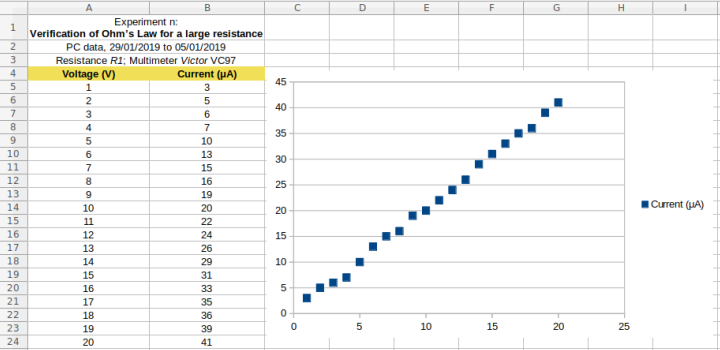
\includegraphics[scale=0.75]{figs/samplegraph1.png}
    \caption{Sample graph of the data in Table (\ref{table:sampledata}) with much to be improved.}
    \label{fig:samplegraph1}
\end{figure}

Excel's biggest user base is business, so default graph formats are mostly setup for that purpose. As a result, changes need to be made to bring it to a `scientific' format: 
\begin{enumerate}
    \item Remove any unnecessary white space. You can do this by adjusting the minimum and maximum values of the axes. You can do this by right clicking the axes and selecting \texttt{Format Axes}.
    
    \item Remove the legend on the right when possible: these are usually just a waste of space. You can select it and press \texttt{Delete}. Any information regarding the graph should be added in the caption.
    
    \item Change the marking icon to a more scientific size and shape. You can right click the graph and select \texttt{Format Data Series} and edit the icon size and shape there.
    
    \item Remove the grid-lines and the tick-marks on the axes.
\end{enumerate}

You should now have a graph like the one shown in Figure (\ref{fig:samplegraph2}).

\begin{figure}[!htb]
    \centering
    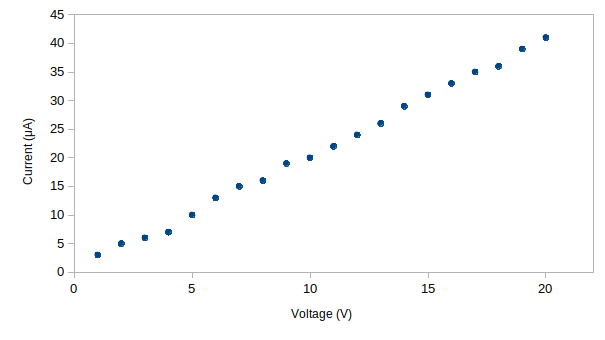
\includegraphics[scale=0.8]{figs/samplegraph2.png}
    \caption{Same graph as in Figure (\ref{fig:samplegraph1}), with some modifications made.}
    \label{fig:samplegraph2}
\end{figure}


\subsubsection{Adding a Trendline}

It should appear to you now that this trend is quite linear. We can now use the computer's algorithm to get the `best' straight line between these points. Don't worry right now about how this is done, you will learn about this in some detail at a later point.

Right-clicking the data-points, select \texttt{Add Trendline}. In the dialog box that opens, choose a \texttt{Linear} regression type and select the checkbox that says \texttt{Show Equation}. You can also make the line dotted, and change its colour. 

If your trendline equation looks something like this:
\begin{center}
    \texttt{f(x) = 0.950310374968518 x - 0.011427047596473}
\end{center}

then edit it to round it off to a more reasonable number of digits. You will understand how many digits is reasonable in the next chapter on error analysis, for right now, let us choose to keep three decimal places. You should now have a graph that looks like Figure (\ref{fig:samplegraph3}).

\begin{figure}[!htb]
    \centering
    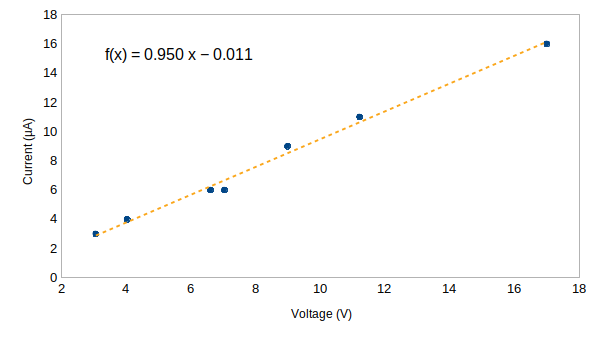
\includegraphics[scale=0.8]{figs/samplegraph3.png}
    \caption{Same graph as in Figure (\ref{fig:samplegraph1}), with formatted trendline.}
    \label{fig:samplegraph3}
\end{figure}

\begin{tip}
In Microsoft Excel, you can make the current graph style a `template', so that you don't have to keep making most of these changes every time you plot new data. To do this, right-click the chart, and select \texttt{Save as Template}. Choose an appropriate name for the chart template and save it. The chart template automatically appears in the \texttt{Templates} folder for charts. You can access it on the \texttt{All Charts} tab in the \texttt{Insert Chart} or \texttt{Change Chart Type} dialog box, where you can apply a chart template like any other chart type.
\end{tip}

\subsection{Graphing with Python}

The purpose of the lab is not to familiarise you to coding with Python -- there is another course that does that. We will be using Python for elementary data analysis. Everything that can be done here can alternatively also be done using Microsoft Excel, so you have a choice of which software to use.



In this section you will learn how to use Python to:

\begin{enumerate}
    \item Import data from CSV files or spreadsheets,
    \item Plot a basic graph,
    \item Add a trendline with its equation.
\end{enumerate}

\subsection{Basic Coding}

As with the other Physics courses, we will be using \textbf{\href{https://jupyter.org}{Jupyter Notebook}}. Go to the link and follow the instruction procedure to install \href{https://www.anaconda.com/downloads}{Anaconda}, a Python distribution that comes with Jupyter pre-installed.

\begin{imp}
The installation of Anaconda Python -- and consequently Jupyter Notebook -- takes a significant amount of time. As a result, you should get it done \textbf{before this session begins}. 
\end{imp}






%\section{Apparatus}



%\section{Description}



%\section{Suggested Procedure}



\newpage
% \chapter{Sensitivity to Errors in Measurement and Preliminary Error Analysis}
\chaptermark{Sensitivity to Errors in Measurement} 
\section{Objectives}

\begin{enumerate}
    \item To recognise different kinds of errors, in particular systematic errors, errors due to the least count of an instrument, random errors, and errors in time measurement.
    \item To learn to use Vernier calipers and the screw gauge.
    \item To begin to understand propagation of errors. 
    \item To use preemptive error analysis to plan an experiment. 
    
    %\item To study the propagation of errors from measured to derived quantities.
\end{enumerate}

\section{Introduction}

When observing the time period of the simple pendulum, you already became aware of the extent to which you are certain of your time measurement. In fact, all the measurements you made -- of mass, of length, of time -- were uncertain. In experimental physics it is of enormous importance to understand how different kinds of errors arise, because without an understanding of errors it is difficult to make sense of data. This is a vast and subtle subject, and so you will learn the elements of it slowly.

It is important to appreciate that in physics \textit{an error is not a mistake}. An error in physics is a measure of how certain (and therefore how uncertain!) we are of a measurement. All measurements are to a greater or smaller extent uncertain; there is no such thing as a perfect measurement: therefore, there is no such thing as an error-free measurement (unless it is something like the \textbf{number of oscillations or rotations}). 

To broaden the scope or your understanding of errors, you will use not only the data you got while observing the oscillations of a pendulum, you will also learn to use two very useful instruments, the Vernier calipers and the screw gauge, which highlight beautifully certain kinds of errors.

\begin{tip}
Example: if you use a metre scale with a least count (smallest division) of $0.1$ cm upside down to measure a pencil and misread the scale as $94.6$ cm instead of $5.4$ cm, this is a \textbf{mistake}.

However, if you note down the length as being $5.4$ cm, but rightly note that it is not \textbf{exactly} $5.4$ cm, but simply that your measuring device does not allow for any more precision, this is a measure of \textbf{uncertainty}. 

We will expect you to have verified that you haven't done the former, and will take for granted from here on that no mistakes were made in the collection of data.
\end{tip}

The complete statement of a measured value \textit{must} include an estimate of the level of confidence associated with the value. This allows people to judge the quality of the experiment and allows for comparisons with other similar estimates of the same quantity, or with theoretical predictions.

\begin{imp}
A proper experiment must report both a ``best'' value and an uncertainty for each measured quantity. You will be expected to do this in all your experiments. 
\end{imp}

Without an uncertainty estimate, it is impossible to answer the basic scientific question: Does my result agree with a theoretical prediction or results from other experiments? This question is fundamental for deciding if a scientific hypothesis is corroborated or refuted.

\section{Systematic Errors} 

Suppose that you are weighing yourself and the pointer is at 1 kg even when no-one is standing on the scales. Then, obviously, all measurements will differ from the correct weights by 1 kg. Such an error is called \text{systematic}, since it appears systematically in all readings. The only way to eliminate a systematic error is to identify its cause and eliminate it. Some devices allow such checking to be done relatively easily, e.g. a metre scale or a weighing scale, but many others do not, e.g. electrical devices with internal errors. Estimating possible errors due to such systematic effects will depend on your understanding of your apparatus and the skill you have developed for thinking about possible problems.  However, if you get a value for some quantity that seems rather far off what you expect, you should think about the possibility of systematic error more carefully. You could end up trusting a device that you do not know is faulty. This happens very often, to the best of us. 

\begin{question}
\paragraph{Question:} You use a ruler whose end is worn out, so that it effectively begins at 2 mm. How can you avoid the systematic error that would arise if you used the ruler naively?

%\vspace{0.5 cm}

\paragraph{Question:} A systematic error can be either positive or negative. What is the difference and under what circumstances would they arise? (If you don't understand this point, you may end up doubling a systematic error in trying to eliminate it.)
\end{question}

\subsection{Least-count-related Errors}

When you make a length measurement with a ruler whose smallest division is 1 mm in size. If you imagine aligning an object of a certain length against a ruler, you can ensure that one end of the object is flush with a mark on the ruler but you cannot ensure that the other end is also flush with another mark -- it general it will be somewhere between two successive marks, and you cannot tell exactly where it is; normally the best that you can do is say, ``It's more than halfway between'', or ``It's less than halfway between''. So the error associated with the least count of the instrument is normally between half and one full least count. 

Because the least count of an instrument is a limitation, one can try to subdivide the region between two marks. It is obvious, however, that this is not going to work beyond a point, since we will simply not be able to tell where the end of the object lies. 

A couple of clever designs \textit{effectively} sub-divide the region. The most beautiful of these designs was first included in an instrument called Vernier calipers; another design is found in the screw gauge. You will learn how to use both of these instruments. (The essential design of the Vernier calipers is incorporated in many other instruments, and we then speak of it as having a Vernier scale.)

\section{Vernier Calipers and the Screw Gauge}

\subsection{Vernier Calipers}

You will regularly come across Vernier scales in the lab when using calipers, angular Vernier scales (in spectrometers), and travelling microscopes. Vernier scales allow you to read off a value more precisely than when using an ordinary scale. In this section, we will explain how this works.

First consider a ``main scale'' with a least count of 1 unit (you could imagine this is 1 mm, if you wish). This implies that any distance between, say, the 2 and 3 unit marks cannot be determined accurately. In other words, the best you could say is that an object is ``2 and a bit'' units. The Vernier scale allows you to \textbf{quantify} this ``bit'' to some extent.  

The method is ingenious: instead of measuring this ``bit'' directly, its magnitude is translated into a a degree of coincidence between two scales, the main scale and a secondary one called the Vernier scale. The Vernier scale has divisions that are \textbf{slightly} smaller than that of the main scale, such that $n$ divisions on the Vernier scale have the same length as $n-1$ divisions of the main scale. For example,  9 divisions on the main scale may coincide with 10 divisions on the Vernier scale (see Figure (\ref{fig:Vernier_1})). 

\begin{figure}[!htb]
    \centering
    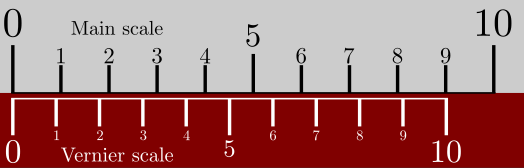
\includegraphics[scale=0.75]{figs/Vernier1.png}
    \caption{10 Vernier scale divisions are set to coincide with 9 main scale divisions.}
    \label{fig:Vernier_1}
\end{figure}

\begin{question}
    \paragraph{Question:} What is the spacing between two Vernier scale divisions? Is it:
    \begin{enumerate}
        \item 1 \texttt{MSD} unit?
        \item 0.1 \texttt{MSD} units?
        \item 0.9 \texttt{MSD} units?
    \end{enumerate}
\end{question}

Let us now try to measure the smallest possible distance between 0 and 1 unit. Take a set of Vernier calipers and close the jaws completely. If there is no zero-error, the only two readings on the Vernier scale which match the main scale are $0$ and $10$, as shown in Figure (\ref{fig:Vernier_1}).

\begin{figure}[!htb]
        \begin{subfigure}[b]{0.5\textwidth}
                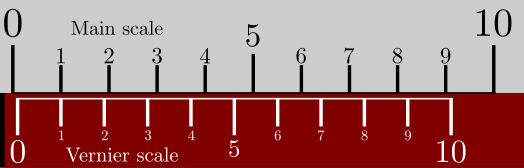
\includegraphics[width=0.95\linewidth]{figs/Vernier2.png}
                \caption{Just away from 0, when the coinciding division is 1, the distance is $1\times\texttt{MSD}-1\times\texttt{VSD}=0.1\, \texttt{units}$.}
                \label{fig:Vernier_2}
        \end{subfigure}\hfill
        \begin{subfigure}[b]{0.5\textwidth}
                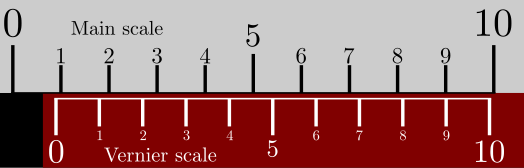
\includegraphics[width=0.95\linewidth]{figs/Vernier3.png}
                \caption{Before crossing 1, the last coinciding division is 9, and the distance is $9\times\texttt{MSD}-9\times\texttt{VSD}=0.9\, \texttt{units}$.}
                \label{fig:Vernier_3}
        \end{subfigure}%
        \caption{Measurement with Vernier Calipers}
        \label{fig:Verniermeasurements}
\end{figure}

\begin{enumerate}
    \item Move the Vernier scale \textit{slightly}, until the $1$ on the Vernier scale coincides with the nearest main scale division (this is obviously the $1$ on the main scale, see Figure (\ref{fig:Vernier_2})). 
    
    \item You will notice that the jaws are slightly apart. The distance between them is of course the distance the $0$ on the Vernier scale has moved. This is the least distance you can measure with this Vernier calliper.
    
    \item But this distance is simply the difference between 1 Main Scale Division (\texttt{MSD}) and 1 Vernier Scale Division (\texttt{VSD}), since both the $1$ marks coincide!
    
    \item Thus, the spacing between the jaws of the calipers is now $1$ $\texttt{MSD} - 0.9$ $\texttt{MSD} = 0.1$ $\texttt{MSD}$ units!
    
    \item We have thus been able to measure a distance of $0.1$ units using two scales, one of least count $1$ unit, and the other of least count $0.9$ $\texttt{MSD}$ units! 
    
\end{enumerate}

Similarly, if you went one division further, and had the 2 of the Vernier scale coincide with a main scale division, then the distance between the jaws would be $2\times\texttt{MSD}-2\times\texttt{VSD}=0.2$ \texttt{MSD} units. Thus, if the $n$th Vernier scale division coincides with a main scale division, the distance between the jaws is $n \times (\texttt{MSD}-\texttt{VSD})=n \times \texttt{LC}$. Where \texttt{LC} is the Least Count of your Vernier calipers.\footnote{In our case, the Least Count is 0.1 \texttt{MSD} units.}

Of course, up until right now we have been measuring distances between 0 and 1 unit.  What about an arbitrary distance? Consider the example given in Figure (\ref{fig:Vernier_4}). 

\begin{figure}[!htb]
    \centering
    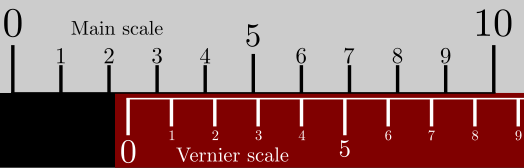
\includegraphics[scale=0.75]{figs/Vernier4.png}
    \caption{The main scale reading is more than 2 units. The coinciding Vernier scale division is 4 (the fact the main-scale reading with which it coincides is 6 is not important).}
    \label{fig:Vernier_4}
\end{figure}

Here is the general procedure to take a reading using Vernier calipers:

\begin{enumerate}
    \item Look for the main scale reading to the left of the the $0$ of the Vernier scale, this is the Main Scale Reading or \texttt{MSR}; the total reading must be this much plus the extra bit between it and the 0 of the Vernier scale. In the example in Figure (\ref{fig:Vernier_4}), the \texttt{MSR} is 2.
    
    \item Now look to find the mark on the Vernier scale which most closely meets any mark on the main scale. This is the Vernier Scale Division or \texttt{VSD}, giving you the most precise digit. In this example, the \texttt{VSD} is 4 because the mark at the end of the 4th division on the Vernier scale coincides with a mark on the main scale (it does not matter which mark on the main scale coincides). If you are still confused, make a movie in your head in which you start with the 0 of the Vernier scale coinciding with a main scale division. Now, slowly, move the 0 of the Vernier scale: First, when the spacing between it and the last main scale division is 1 LC, the first \texttt{VSD} will coincide with a main scale division, then, when that spacing is 2 LC, the \textit{second} \texttt{VSD} will coincide with \textit{another} main scale division, and so on.
    
    
    \item The total distance is given by 
    \begin{equation*}
    \begin{aligned}
    \texttt{distance} &=& \texttt{MSR} &+ (\texttt{VSD}\times\texttt{LC})
    &=&0.2 &+ (4 \times 0.01) = 0.24
    \end{aligned}
    \end{equation*}
    
    In our case, $\texttt{distance} = 0.24$ \texttt{MSD} units.
    
    \item Thus, using two scales -- one of least counts $1$ unit and another of least count $0.9$ units -- we have calipers capable of measuring up to (or down to!) $0.1$ units! You have an \textit{effective least count} that is much smaller than the least count of the main scale. 
\end{enumerate}

\begin{question}
\paragraph{Question:} Show that the least count of a set of Vernier calipers is given by:
\begin{enumerate}
    \item $$\texttt{LC} = \texttt{Least count of main scale} - \texttt{Least count of Vernier scale}$$
    \item $$\texttt{LC} = \frac{\texttt{Least count of main scale}}{\texttt{Number of Vernier scale divisions}}$$
\end{enumerate}
\end{question}

\subsection{The Micrometer Screw Gauge}

The design of the micrometer screw gauge is different, and uses the fact that a linear movement that is imperceptible can be turned into an angular movement that is easily perceptible; the best way to understand this is simply to examine the screw gauge (which, unlike Vernier calipers, is easy to understand). The screw gauge uses a screw with an accurate and constant \textbf{pitch} (the amount by which the thimble moves forward or backward for one complete revolution) as an auxiliary scale marked on a rotatable thimble.  

The micrometers in our laboratory have a pitch of $0.5$ $\mathrm{mm}$.  The rotating thimble is subdivided into 50 equal divisions.  The thimble passes through a frame that carries a millimetre scale graduated to $0.5$ $\mathrm{mm}$.  The jaws can be adjusted by rotating the thimble using the small ratchet knob.  This includes a friction clutch which prevents too much tension from being applied.

\begin{imp}
Only tighten the screw gauge by rotating the ratchet, otherwise you may damage the instrument. Stop rotating after you hear \textbf{three} clicks. \textbf{Do not} tighten the screw any further.
\end{imp}

\begin{question}
\paragraph{Question:} Show that the least count of a screw gauge is given by
$$\texttt{LC} = \frac{\texttt{Pitch of a the screw}}{\texttt{Number of circular scale divisions}}$$
\end{question}

\section{Random Errors}

Let us go back the simple measurement of the length of an object with a ruler. We place the object against the ruler with one end flush against a certain division of the ruler, say 0 (it does not have to be 0, but usually is). Then we observe where the other end is. In general, it will be, as mentioned earlier, at some point between two successive marks on the ruler. Let us imagine doing this repeatedly. Every time we place one end against 0, it will be at \textit{slightly} different point, and so the other end will also move slightly, in a manner that we cannot control. If this movement is much smaller than the distance between two successive marks on the ruler, i.e. its least count, then this random movement will not be discernible. On the other hand, if the movement is greater than the least count of the ruler, then the length we measure will change from one measurement to the next. In the first case the error is determined by the least count of the ruler, and the length measured will not change from one measurement to the next. In the second case, however, it is clear that the length measured \text{will} change from one measurement to the next. We call this kind of error a \textit{random error}.

Another example that may make the idea clearer is the following. Imagine that a sound of a fixed duration is played over and over again, and you are required to time the duration with a stopwatch. You will have to start and stop your stopwatch over and over again. It is easy to see that even though the duration of the sound remains the same, the duration that you measure will vary from one measurement to the next. Once again we have a random error. It should be intuitively clear that the magnitude of the error depends not on the duration of the sound but on the \textit{spread} of your measurements. The number we assign to the random error must therefore be obtained from a measure of this spread. To do this, we must remove what does not matter, namely the actual duration of the sound. Generally we don't know the actual duration of the sound. So we do the best we can: we subtract the mean of our measurements from all of them, since the mean is our best guess of the actual duration. That leaves us a distribution of the variations of the measurements. 

We are not really concerned with whether the variation is positive or negative. So we use the sum of the squares of the variation, i.e. $\sum_{i = 1}^{n}(x_i - \overline{x})^2$, where $x_i$ is any reading, $\overline{x}$ is the mean, and $n$ is the total number of readings. Because the variations are both positive and negative, this sum grows not in proportion to $n$ but in proportion to $\sqrt{n}$. (This is a subtle point; you will understand it later.) So the standard measure of the spread of the readings is the standard deviation 
\begin{equation*}
    \sigma = \sqrt{\frac{\sum_{i = 1}^{n}(x_i - \overline{x})^2}{n - 1}}.
\end{equation*}

(Why $n-1$ instead of $n$ in the denominator is another subtle point. Again, let it be for the moment. Anyway, the difference between $n$ and $n-1$ is negligible for large $n$, which is the only case in which the idea of random errors is meaningful.)

\section{Errors in Time Measurements}

The time measurements you will encounter in the lab will be made by human beings (you) using clocks. If you compare the processes of measuring a duration to that of measuring a length, you will immediately see that you no longer have the luxury of aligning one end of your ``object'' (here a duration) with a physical scale: you must start your clock at a moment that you best judge to be the beginning of the duration and end it at what you best judge to be its end. Thus you automatically make two errors, one at the end of your time measurement and one at the beginning. The magnitude of the error has nothing to do with how long or short the duration is. 

Is this error due to the least count of you clock? It is -- partly; but that's not the whole story: there is another factor to take into account, your reaction time. As a human being you have to judge when when the duration begins and press the start button on your clock; both your judgement and the pressing of the button entail errors that are due to the finite time it takes for your brain and your body to react. Thus the errors at the beginning and the end of a measurement of duration are a combination of the the error due to the least count of your clock and your reaction time. If one is much larger than the other, it dominates and the other may be neglected. 

Determining the least-count error is easy: it's just the last count of your clock. Determining the error due to finite reaction time is not easy. One way is to do many measurements of a duration that is known to be constant (e.g. the period of a pendulum) and look not at the average but the spread in the readings, a measure of which is the standard deviation. For most human beings have a reaction time of about 0.1 $s$, much larger than the least count of standard lab stop watches, which is usually 0.01 $s$. Thus the error in most of your time measurements will be dominated by your reaction time. 

\subsection{Time Measurement for Periodic Phenomena}

You will often be interested in measuring a duration of a periodic phenomenon, e.g. the oscillation of a pendulum. If you assume that the period of the pendulum has a true value that does not change from one oscillation to the next, then there is a way in which you can dramatically reduce the error on the time period. Since the error in the measurement of a duration occurs only at the ends, you can simply measure the duration for many oscillations, e.g. 10 or 100, and divide by that number. So, if the total error due to your reaction time on a duration (i.e at both ends of a duration together) is 0.1 $s$ and you measure the duration for 10 oscillations, the error associated with a single time period will be $0.1/10 = 0.01 s$.

Given that this is true, you may ask why one doesn't simply measure the duration for 1000 oscillations (or some arbitrarily large number). One answer is that the oscillations will damp out. The other had to do with human fatigue: if you are asked to count 1000 oscillations, you may make an error in counting the number of oscillations, and that would lead to a much larger loss in precision than what you gained by increasing the number of oscillations. (Machines don't have this problem and it makes sense, when a mechanical counter is being used, to increase the number of oscillations as much as possible.) 

A question that might arise is what happens if we measure the duration for 10 oscillations several times. Is this equivalent to measuring the duration for 100 oscillations? No. Now we have a pair of end points for each duration of 10 oscillations, and each point is associated with starting and stopping a clock. If we measure the duration for 100 oscillations (let us call this case 1), we have 2 end points, and if we measure 10 sets of 10 oscillations each (case 2), we have 20 end points, i.e. there are 10 times as many points at which errors can occur. From this we may at first conclude that the error in case 2 is 10 times the error is case 1, but that is not correct: the errors we make at the end points can be either overestimates of underestimates, i.e. positive or negative, and so as we stack up the end points there will be some cancellation. It an be shown -- and at some point you will show this -- that as the number of end points $n$ increases, the error goes up as $\sqrt{n}$. Thus, if the error on time measurement with single pair of end points is $\Delta t$, the error on combining $n$ time measurements is $\sqrt{n} \, \Delta t$. Putting all this together, if the error on a single time measurement is $\Delta t$, the error on the time period $T$ using 100 oscillations is $\frac{\Delta t}{n}$ and the error on $T$ using 10 measurements of 10 oscillations each is $\frac{\sqrt{n} \, \Delta t}{n} = \frac{\Delta t}{\sqrt{n}}$. (Don't worry if this paragraph went over your head; you will understand it slowly, over the semester.)

It should be obvious from the discussion above that while time measurement is much more subtle than length measurement, it allows an almost arbitrary improvement in precision (reduction in error) on the time period itself (to be distinguished from the duration of a measurement)  if the phenomenon is periodic. This can be used to great effect in certain devices, e.g. the Kater's pendulum. To ensure that this great advantage is not vitiated by incorrect counting of oscillations, it is very important to know exactly how to count the number of oscillations. A very common error is to count $n-1$ oscillations when one wants to count $n$. You will learn the correct procedure in the lab. 

%\section{Theory: Error Analysis}

%\subsection{Types of Errors}

%``Error'' analysis is a rather glaring misnomer. All measurements have some degree of uncertainty that may come from a variety of sources, from the lack of precision of the measuring instrument to random fluctuations in the environment. The process of evaluating the uncertainty associated with a measurement result is often called uncertainty analysis or error analysis. However, the common definition of an ``error'' being a ``mistake'' is very misleading. However, the terminology is so rampant that we will be forced to use it at times, referring to ``error'' analysis when we really mean ``uncertainty'' analysis.


\begin{tip}
\paragraph{A cautionary tale:} Neutrinos are weakly interacting nearly massless particles that are theorised to be moving close to -- if not at -- the speed of light.

In September 2011, scientists of the OPERA collaboration reported evidence that neutrinos they produced at CERN in Geneva and recorded at the OPERA detector at Gran Sasso, Italy, had travelled \textbf{faster} than light. If this were true, it would have violated one of the pillars of modern physics, the Theory of Relativity.

The neutrinos were calculated to have arrived approximately 60.7 nanoseconds sooner than light would have if it had traversed the same distance in a vacuum. Assuming the error were entirely due to random effects, scientists calculated that there was a 0.2-in-a-million chance that this may be a false positive.

In March 2012 it was confirmed that a fibre cable was not fully screwed in during data gathering, and this effectively decreased the reported flight time of the neutrinos by 73ns, making them seem faster than light. The corrected difference between the measured and expected arrival time of neutrinos (compared to the speed of light) was approximately 6.5 $\pm$ 15 ns. This is consistent with \textbf{no difference at all}, thus the speed of neutrinos is consistent with the speed of light within the margin of error.
\end{tip}

%\subsubsection{Least count errors}

%As you have already seen, the least count of a measuring instrument is the smallest value the instrument can resolve. For example, if we use a metre scale to measure an object and find that it is $23.5$cm, the uncertainty here \textbf{due to the measuring instrument} is $0.1$cm. Thus, we can say that the length of the object is given by $l = (23.5 \pm 0.1) cm$ where $\pm \Delta l = \pm 0.1$cm is the uncertainty in measurement due to the least count of the metre scale. This is the value up to which the ``best'' value of $23.5$ may be specified with any confidence.

%In general, such errors are the \textbf{lower bounds} of experimental errors. No error that is less than the least count error need be considered. That being said, if you find other sources of error to be greater than the least count error, then those sources should be used. For example, the stopwatches in the lab have a least count of $0.01$s. However, your reaction time of turning on and off a stopwatch would be at best $0.1$s. Thus, while the least count error is significantly smaller, the \textbf{actual} error in a time measurement using the stopwatch would be of the order of $0.1$s.

%\subsubsection{Systematic errors}

%Imagine now that the metre scale that you are using to measure the length of the object is made of metal, and as a result expands slightly in summer. If you performed a set of measurements, you would obviously not find the ``true'' value of the length. However, such an error may be discovered by comparing your measurements from the metal scale with a wooden scale, for example. When using instruments like digital multimeters you obviously rely on it having been calibrated properly. However, there might have been an accident that a student did not report, and as a result there could well be a systematic error for someone unlucky enough to be the one using it next.

%\subsubsection{Random errors}

%Another reason for two measurements not agreeing totally is due to small, uncorrelated variations in the environment or measurement process. For example, while measuring the time period of a pendulum, you might get different readings due to small differences in your reaction time. Similarly, when measuring the height of a cylinder with a Vernier calliper, you may see small variations depending on \textbf{where} you measure the height, as it is possible the cylinder was not made to be smooth up to $0.1$mm everywhere.

%Such variations, being \textbf{random}, are expected to fall just as often \textit{above} a certain value as \textit{below} it. A truly random source would give you a \textbf{Gaussian} distribution of errors; the mean of this distribution $$\overline{m}_N = \frac{\sum_{i=1}^{N}{m_i}}{N}$$ would approach the ``best'' value as the number $N$ of well-sampled values increases. The uncertainty of these measurements would then be quantified by the \textbf{standard deviation}\footnote{There is a reason for the $N-1$, it is known as the number of ``degrees of freedom'' in statistics. Understanding it is not essential for this course.} $$\Delta m_N = \sqrt{\frac{(m_i - \overline{m}_N)^2}{N-1}}$$

%more conventionally denoted by $\sigma$.

\subsubsection{Precision, Accuracy, and Statistics}

\begin{enumerate}
    \item \textbf{Accuracy:} is how closely a measurement comes to some ``true'' value. It determines how well we have eliminated \textbf{\textit{systematic errors}} and mistakes in our measurements.
    \item \textbf{Precision:} is how closely a set of measurements agree \textit{with each other}. %It determines how well we have eliminated \textbf{\textit{random errors}} in our measurements.
\end{enumerate}

To use a sports simile, if you're playing football and are accurate, your aim will always take the ball close to or into the goal. If, however, you harbour a personal grudge against the coach and succeed in beaning him on the head every time you get the ball, then you would be \textit{precise}, but not accurate.\footnote{It is widely accepted that the point of football is to get the ball into the goal and not to traumatise your coach, which is why this example works.}

\textbf{A caveat:} In any physics experiment worth doing, you usually don't have the answer beforehand. This means you don't have a ``true'' value with which to compare your answer. This is why it is so important to be both precise (reduce all random errors present in your measurements) and accurate (reduce all systematic errors present in your measurement). You must also, however, come up with ways to check if your answer is accurate \textit{without} trying to resort to a ``textbook'' solution.

\begin{question}
\paragraph{Question:} In the example of the ``superluminal'' neutrinos given earlier, was the error of the OPERA team one of inaccuracy, or of imprecision? 
\end{question}

\section{Propagation of Errors}

In general we are interested not just in our observations but in quantities derived from them, i.e. in derived quantities. It is obvious that the a derived quantity will inherit some the errors in the observations from which it is derived. But to what extent will it do so? We will use a few examples to understand this. 

\begin{enumerate}
    \item We want the radius of a diameter, we usually measure its diameter. Here the observed quantity is the diameter $d$ and the derived quantity is the the radius $r$. We have $r = d/2$. Thus if there is an error of $\pm \delta$ in measuring $d$ (for example due to the least count of the measuring instrument), then, clearly the error in $r$ is $\pm \delta/2$.
    
    \item We want the perimeter $p$ of a rectangle having measured its length $l$ and its width $w$. $p = 2l + 2w$. If the errors in measuring $l$ and $w$ are $\pm \delta$, for each, the error in $p$ is clearly $\pm 2 \delta \pm 2 \delta$, which ranges between $- 4 \delta$ and $+ 4\delta $, depending on the signs on the errors on $l$ and $w$. So the error on $p$ is $\pm 4 \delta$.
    
    \item We want the area $A$ of a rectangle having measured its length $l$ and its width $w$. $A_\text{true} = l \, w$. Suppose that the error in the measurement of $l$ is $\pm \delta l$ and the error in measuring $w$ is $\delta w$, then what we derive is $A_\text{derived} = (l \pm \delta l) (w \pm \delta w)$. If the errors are much smaller than measurements, we can neglect terms of order $\delta^2$. Then, the value of $A_\text{derived}$ ranges between $A_\text{true} - w \delta l - l \delta w$ and $A_\text{true} +  w \delta l + l \delta w$. Notice that the expression for the error is rather complicated; we can simplify it if we express it in terms of the relative error. Since the error in $A$ is $\delta A = A_\text{derived} - A_\text{true}$, you can easily show that 
    \begin{equation*}
        \frac{\delta A}{A} = \pm \frac{\delta l}{l} \pm \frac{\delta w}{w}.
    \end{equation*}
    The quantity $\delta x / x$ is called the \textit{relative error} in $x$.
    
    \item We want the volume $V$ of a sphere given a measurement of its diameter $d$. You can easily show, using the method given above, that 
\begin{equation*}
    \frac{\delta V}{V} = \pm 3 \, \frac{\delta d}{d}.
\end{equation*}
Notice how the sensitivity of the relative error in $V$ to the relative error in $d$ depends on the \textit{power} in the dependence of $V$ on $d$. (Since $V = (4/3) \pi r^3$, $V \propto d^3$.)
    
    \item We want the mass per unit length $\lambda$ of a wire having measured its mass $m$ and its length $l$, with . $\lambda_\text{true} = (m \pm \delta m) / (l \pm \delta l)$. If you go through the same process as in the last case considered, you will find that 
    \begin{equation*}
        \frac{\delta \lambda}{\lambda} = \pm \frac{\delta m}{m} \pm \left( -\frac{\delta l}{l} \right).
    \end{equation*}
    
\end{enumerate}

\section{Using Error Analysis to Plan Your Experiment}

Suppose that you want to measure the volume of a tile (whose length $l$ and width $w$ are much greater than its thickness $t$). Since $V = l \times w \times t$, you have
\begin{equation*}
    \frac{\delta V}{V} = \pm \frac{\delta l}{l} \pm \frac{\delta w}{w} \pm \frac{\delta h}{h}.
\end{equation*}
This formula shows you right away that there is not much point improving one measurement indefinitely if the dominant cause of error is another measurement. What we want is for all the measurements to contribute more or less equally. This immediately tells us that we must choose our instruments and number of measurements so that this goal is achieved. 

\begin{question}
\paragraph{Question:} What instruments would you choose measure the length, width, and thickness of the tile so that the relative errors in them are comparable?

%\vspace{0.5 cm}

\paragraph{Question:} Suppose $P = x y^3$, where $x$ and $y$ are the measured quantities. On which of them is the relative error in $P$ more sensitive?

\end{question}
\newpage
\section{The Experiment}

\subsection{Apparatus}

\begin{enumerate}
    \item A pair of Vernier calipers
    \item A Screw gauge
    \item A set of ball bearings
    \item A set of aluminium cylinders
    \item A small measuring flask
    \item A container with a spout
\end{enumerate}

\subsection{Description}

\begin{enumerate}
    \item In \textbf{Part A} you will measure the radius, height, and volume of different cylinders. You will then plot an appropriate graph from which you will extract the value of $\pi$.
    
    \item In \textbf{Part B} you will measure the radius and volume of different ball bearings. You will then plot an appropriate graph from which you will extract the value of $\pi$.
    
\end{enumerate}

\subsection{Suggested Procedure}

\subsubsection{Part A}

\begin{enumerate}
    \item Decide on the best instrument and method to measure the following properties of the cylinders:
    \begin{enumerate}
        \item Radius
        \item Height
        \item Volume
    \end{enumerate}
    
    \begin{question}
        \paragraph{Question:} How and where would you measure the radius of the cylinders? How many trials would you take?
    \end{question}
    
    \item Be sure to take a sufficient number of \textbf{well-sampled} readings.
    
    \item Decide on an appropriate graph between the measured quantities from which you can extract the numerical value of $\pi$.
\end{enumerate}

\subsubsection{Part B}

\begin{enumerate}
    \item Decide on the best instrument and method to measure the radii and the volumes of the bearings.
    
    \item Be sure to take a sufficient number of \textbf{well-sampled} readings.
    
    \item Decide on an appropriate graph between the measured quantities to extract the numerical value of $\pi$.
\end{enumerate}

\begin{question}
\paragraph{Question:} How does your estimate compare with the known value of $\pi \approx 3.14159$?
\end{question}



\newpage



% \vbox{
% \textcolor{Blue}{\part{Experiments}}
% \tikz[remember picture,overlay]\node[shift={(-1,1)},opacity=0.6] at (current page.south east) {
\includegraphics[width=17.5cm]{logo}};
% }

% \renewcommand{\chaptername}{Experiment}

% % \title{The Soft Massive Spring}
% \author{An Introduction to Physics through Experiments}
% \date{}
% \maketitle

\chapter{The Soft Massive Spring}

\section*{Objectives}

\begin{enumerate}
\item To determine the spring constant and the mass correction factor for the given soft massive
spring by static (equilibrium extension) method.
\item To determine the spring constant and the mass correction factor for the given soft massive
spring by dynamic (spring mass oscillations) method.
\item To determine the frequency of oscillations of the spring with one end fixed and the other
end free i.e. zero mass attached.
\item To study the longitudinal stationary waves and to determine the fundamental frequency of
oscillations of the spring with both the ends fixed.
\end{enumerate}

\section*{Introduction}

Springs are familiar objects with many everyday applications ranging from retractable ballpoint pens, to weighing scales and metro handles. Let us consider an ideal spring: such a spring has an equilibrium length -- that is, a length when no external force is applied -- and resists any change to this length through a restoring force.

%\todo[inline]{Diagram showing forces and springs.}

\begin{figure}[!htb]
    \centering
    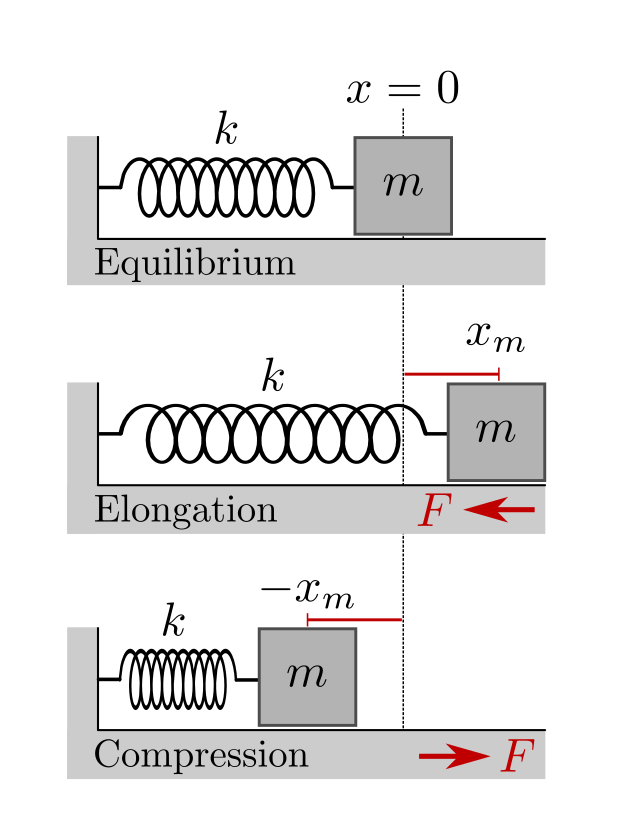
\includegraphics[width=0.4\textwidth]{figs/springForce.png}
    \caption{The restoring force experienced by the mass due to the spring is proportional to the amount the spring is stretched from its equilibrium position.}
    \label{fig:springForces}
\end{figure}

In such ideal springs, the force required to stretch (or compress) is assumed to be proportional to the amount which the spring is stretched (with compression being negative stretching). When one end is fixed, then this stretch is just the displacement of the free end. From now on we will assume that one end is fixed (which implies that we must use the formulas carefully when both ends are free). This tells us that the restoring force i.e.\ $F \propto x$. By defining a constant of proportionality $k$, known as the spring constant, we can write down \textit{Hooke's Law}:

\begin{equation}
    F = - k x,
    \label{hooke}
\end{equation}

where the negative sign shows that the force is in the direction opposite to the displacement of the end, i.e.\ it is a restoring force: when the spring is stretched, this force tends to compress it, and vice versa. Experiment reveals that for relatively small displacements, almost all \textit{real} springs obey Equation (\ref{hooke}).

Let us assume that the spring is placed horizontally on a frictionless surface and attached to a wall on one end and an object of some mass $M$ on the other, which we can pull or push. If we displace the object by some $x$ and let go, it will experience a restoring force due to the spring, which will change as the object begins moving. Combining Newton's Second Law and Equation (\ref{hooke}) we can see that the acceleration of the object is given by

\begin{equation}
\begin{aligned}
    a &= \frac{F}{M} \\
    \dv[2]{x}{t}&=-\frac{k}{M} x
\end{aligned}
\label{diffEqnSimpleSpring}
\end{equation}

where we have chosen $x = 0$ as the equilibrium position of the mass (in which the spring has its unstretched, or equilibrium, length).

%\todo[inline]{Diagram showing horizontal oscillations.}

It is not difficult to see that any function whose second derivative is itself (times a negative constant) is a solution to the differential equation above. Both $\sin (\omega t)$ and $\cos (\omega t)$ are such functions. From the theory of differential equations, we know that the general solution to this differential equation is a linear combination of two linearly independent solutions. Thus we can write

\begin{equation*}
    x(t) = A \sin(\omega t) + B \cos(\omega t),
\end{equation*}

where $\omega$ -- known as the frequency of vibration -- must be equal to $\sqrt{k/M}$ for the left and right sides to match, and $A$ and $B$ are constants determined by the initial conditions (initial position and initial velocity). Observing the solution above, it should be clear to you (since $\sin$ and $\cos$ are periodic functions) that there must be some time $T$ after which $x(t)$ comes back to itself, i.e.\ $x(t+T) = x(t)$. The motion is thus periodic, with period equal to that of the sinusoidal functions $\sin(\omega t)$ and $\cos(\omega t)$, which is

\begin{equation}
    T = \frac{2 \pi}{\omega} = 2\pi \sqrt{\frac{M}{k}}.
    \label{masslessTime}
\end{equation}

The mass thus oscillates about its equilibrium position with a time period $T$ that is -- at least for small amplitudes -- independent of amplitude.

%\todo[inline]{Diagram showing twice the mass and twice the displacement under gravity.}

\begin{figure}[!htb]
    \centering
    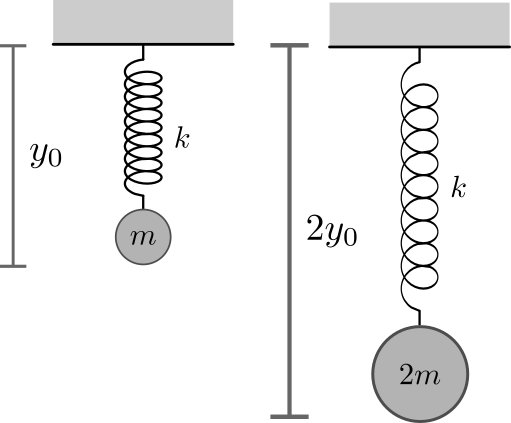
\includegraphics[width=0.3\textwidth]{figs/springMassVertical.png}
    \caption{Hanging vertically, if a mass $m$ causes the spring to extend to $y_0$, a mass of $2m$ will cause the same spring to extend to $2 y_0$.}
    \label{fig:springMassVertical}
\end{figure}


We could now imagine hanging the spring and mass vertically. While the spring is assumed to be massless (as it is ideal), the massive object experiences a downward force due to gravity of $Mg$. At static equilibrium, the spring would have displaced enough to balance this force. Thus,

\begin{equation}
    y_0 = \frac{Mg}{k}.
    \label{masslessExt}
\end{equation}

We could similarly gently displace this spring vertically about this position, and we would again see oscillations, only this time the oscillations will be about the point $y_0$, which is the new equilibrium point.

\begin{figure}[!htb]
    \centering
    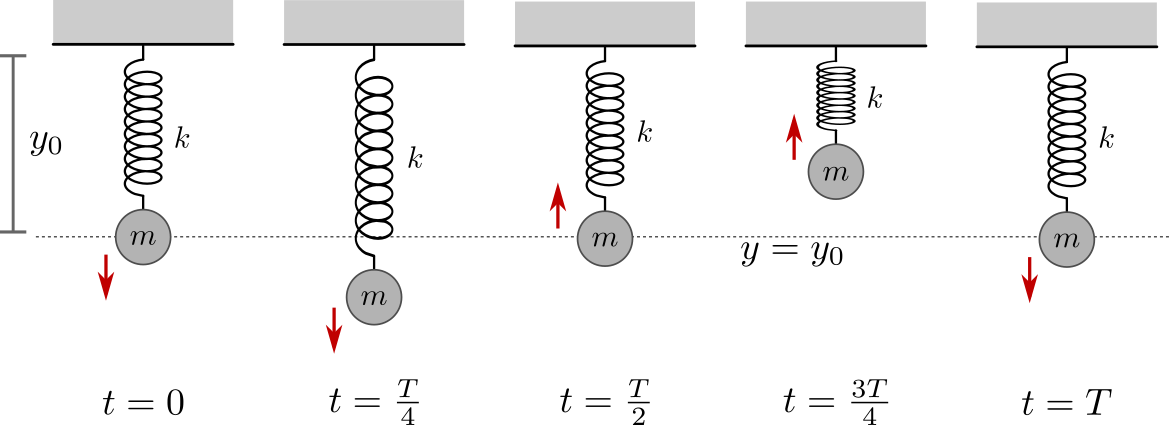
\includegraphics[width=\textwidth]{figs/springOscillations.png}
    \caption{If the vertically hanging spring is displaced slightly, it will begin to oscillate with a time period $T$ about the new equilibrium point $y_0$, as shown.}
    \label{fig:springOscillations}
\end{figure}


\begin{question}
\paragraph{Question:} Write out Newton's Law as a differential equation in this case (i.e.\ when gravity is included). Show that it can be written as:

\begin{equation*}
    \dv[2]{y}{t} = -\omega^2 (y - y_0) 
\end{equation*}

\paragraph{Question:} By making a suitable substitution and comparing it with Equation (\ref{diffEqnSimpleSpring}), show that the solutions have the same form in a shifted variable.

\paragraph{Question:} Show that the time period $T$ is the same as in the preceding case (of ``static'' equilibrium).
\end{question}


\subsection*{Massive springs}

So far, we have assumed our spring to be ``massless'', in that its mass may be neglected. Whether or not this is a reasonable assumption does not depend on the spring alone, but on external factors. 

On inspection, it should be clear to you that the top and the bottom of a spring hung vertically do not experience the same downward or restoring forces, even at static equilibrium.\footnote{In general, a spring is not a ``rigid'' body.} If this ``droop'' (caused by the mass of he spring) is negligible compared to the stretch caused by external masses, then the spring may be effectively considered as massless. Thus it depends roughly on the ratio of the masses.


\subsubsection*{The static case}

Let us consider a point very close to the top of the spring: it will experience a (small) restoring force from the small amount of spring above it, and a much larger downward force from the mass of spring under it. Similarly, consider a point very close to the free end of the spring: it will experience a larger restoring force (as there is more ``spring'' above it) than downward gravitational force as there is very little mass under it. As a result, the spring does not stretch uniformly; the coils near the top are further separated than those near the bottom. We would thus expect some form of ``correction factor'' to the mass term in Equation (\ref{masslessExt}).

Consider a spring with some mass $m_s$. Let $L_0$ be the length of the spring when it is kept horizontally with no forces extending it, and $L_M$ be the length of spring when it is hung vertically with a mass $M$ attached to its lower end. We can define the ``equilibrium extension'' $S_M$ as

\begin{equation}
S_M = L_M - L_0.
\end{equation}

It is possible to solve the problem theoretically and show that the massive spring acts effectively like an ideal spring with a mass $m_s/2$ attached to its end. In other words, if a massive spring is hung vertically, and an ideal spring with mass $m_s/2$ is attached to its end, they will both extend to the same distance.

Thus, Equation (\ref{masslessExt}) is modified to

\begin{equation}
S_M = \left( M + \frac{m_s}{2} \right)\left(\frac{g}{k} \right)
\label{Sm}
\end{equation}

where the factor $m_s/2$ is known as the \textbf{static} mass correction factor.


\subsubsection*{The dynamic case}

Consider now the case of an ideal spring oscillating with a mass attached at its end. The oscillating mass $M$ will have a kinetic energy 

\begin{equation*}
    K_\text{mass} = \frac{1}{2} M v^2
\end{equation*}

However, if the spring itself is massive, since different parts of it move at different velocities, it will also have some kinetic energy associated with it. To find the total kinetic energy of the spring, one could imagine an infinitesimal mass element on the spring moving at some velocity and integrate its contribution to the kinetic energy to get the total energy:\footnote{Though this is slightly advanced, it is not too difficult to do at your level. We urge you to attempt to show this theoretically.}

\begin{equation}
    K_\text{spring} = \frac{1}{6} m_s v^2
\end{equation}

\begin{imp}
This also explains why the spring oscillates even when it has no external mass attached.
\end{imp}

\begin{question}
\paragraph{Question:} Show, from the earlier expressions for kinetic energy, that the spring behaves like an ideal spring with a mass of $m_s/3$ attached to it.
\end{question}

Thus, when an external mass $M$ is attached to the spring, it behaves as if it is effectively an ideal spring with a mass $M+ m_s/3$ attached to its end. Thus, Equation (\ref{masslessTime}) will need to be modified.

The resulting time period $T$ for the oscillations of a massive spring is given by 

\begin{equation}
T = 2\pi \sqrt{\cfrac{\left(M + \cfrac{m_s}{3}\right)}{k}}.
\label{Tm}
\end{equation}

The factor $m_s/3$ is the \textbf{dynamic} mass correction factor. 

\begin{imp}
Note that this factor is different from the mass correction factor in the previous (static) case. The reason for this difference is that they arise from two different processes. In the first case, the effective mass comes from the fact that the different mass-elements comprising the spring experience different forces, which affects the effective \textit{extension}. In the dynamic case where these different mass-elements are \textit{moving}, the term $m_s/3$ comes from the fact that they have different velocities, which affects the effective \textit{kinetic energy}.

%\todo[inline]{Could still use some work.}
\end{imp}

\begin{question}
\paragraph{Question:} Show that if the mass $M$ that is attached is too large compared to $m_s$, Equations (\ref{Sm}) and (\ref{Tm}) give the same results as for an ideal spring. 
\end{question}


When no additional mass is attached to the spring (i.e.\ $M=0$), we can define a corresponding frequency for the massive spring  

\begin{equation}
    f_0 = \frac{1}{T} = \frac{1}{2\pi} \sqrt{\frac{3k}{m_s}}.
\end{equation}


\subsubsection*{Standing waves on a massive spring}

If we stretch the spring between two fixed points, it can be considered as a system with a uniform mass density (say, number of rungs per centimetre). When vibrated with some periodic forcing, this system has its own natural frequencies, very much like sound waves in a hollow pipe closed at both ends.\footnote{The pipe being ``closed'' implies that the amplitude of the waves at both ends is zero. In this case, the top end of the spring is fixed, and the bottom end moves at an amplitude so small compared to the length of the spring, that it can effectively be considered to be fixed.}

\begin{figure}[!htb]
    \centering
    \begin{subfigure}[b]{0.5\textwidth}
        \centering
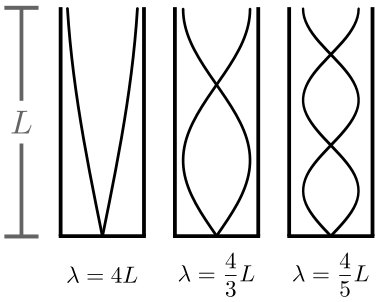
\includegraphics[width=0.8\textwidth]{figs/wavesInAHalfOpenPipe.png}
                \caption{Waves on a pipe with one closed and one open end.}
                \label{fig:wavesInAHalfOpenPipe}
        \end{subfigure}\hfill
        \begin{subfigure}[b]{0.5\textwidth}
        \centering
                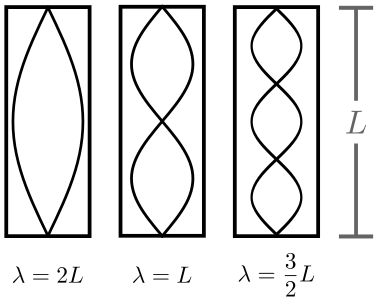
\includegraphics[width=0.8\textwidth]{figs/wavesInAClosedPipe.png}
                \caption{Waves on a pipe with both ends closed.}
                \label{fig:wavesInAClosedPipe}
        \end{subfigure}
    \caption{Variation of amplitude in an air column: Sound waves are characterised by a series of alternate compressions and rarefactions. When an end is closed, the air particles there do not move, and thus that point is a node. Conversely, when the end is open, the particles have the maximum amplitude, and so that point is an antinode.}
    \label{fig:wavesInAPipe}
\end{figure}


When this system is vibrated at one of these ``natural'' frequencies, standing (longitudinal) waves are seen to form, with clear nodes -- i.e.\ points on the spring that remain completely stationary. Two important points can be noticed about the nodes in this case:

\begin{enumerate}[label=(\alph*)]
    \item They divide the length of the spring into equal parts.
    \item They increase by 1 as you move from one natural frequency to the next.
\end{enumerate}

\begin{question}
\paragraph{Question:} Drawing out a diagram like Figure (\ref{fig:wavesInAPipe}), show that the wavelength of a wave with $n$ nodes is given by

\begin{equation}
    \lambda_n = \left(\frac{2}{n+1}\right) L , \quad \quad n=0,1,2\hdots
\end{equation}
where $L$ is the length of the column and $n$ the number of nodes (excluding the fixed endpoints).
\end{question}


We know that waves satisfy the following equation that relates their wavelengths and frequencies, 

\begin{equation}
    v = f_n \lambda_n
\end{equation}

where $v$ is the velocity of the wave. As this is a constant for a configuration, it follows that 

\begin{equation}
\begin{aligned}
f_n = \frac{v}{\lambda_n} &= \frac{v (n+1)}{2L}\\
f_1 = \frac{v}{2L}, \quad f_2 = \frac{v}{L},\quad &\hdots,\quad f_n = n f_1.
\end{aligned}
\end{equation}



\section*{Experimental Setup}

\subsection*{Apparatus}

\begin{enumerate}[label=\arabic*)]
\itemsep0em
\item A set of soft massive springs
\item A long and heavy retort stand with a clamp at the top end 
\item A set of masses with hooks
\item A signal generator (\textit{Equip-tronics QT-210})
\item A dual output power amplifier with the connecting cords
\item A mechanical vibrator
\item A digital multimeter (\textit{Victor VC97})
\item A digital stopwatch (\textit{Racer})
\item Measuring tapes
\item A set of measuring scales (1.0 m, 0.6 m and 0.3 m)
\end{enumerate}

\subsection*{Description}

\begin{description}

\item[Digital Multimeter (\textit{Victor VC97})]

A multimeter is an instrument used to measure multiple parameters like voltage, current, and resistance. You will be using the multimeter to measure the frequency of the signal. You will have to use input sockets marked COM, V/$\Omega$ to do this. Note that the two input sockets marked mA and 10A are for the current measurement. You will not be using those. Connect the banana cables to COM and V/$\Omega$, and select the Hz setting on the multimeter. 

\item[Signal Generator]

A signal generator is used to generate simple repetitive waveforms in the form of an alternating electrical wave. Typically, it will produce simple waveforms like sine, square, and triangular waves, and will allow you to adjust the frequency and amplitude of these signals. The instrument given to you generates sine, sawtooth, and square waveforms. The output may be taken from the respective output sockets through banana cables. The frequency can be adjusted by turning the frequency dial and turning the Range knob to the appropriate multiplier. For example, turning the dial to 3 and selecting the 100X setting in the range knob would provide an output waveform with a frequency of 300Hz. Similarly the amplitude knob varies the amplitude of the output waveform.

\begin{tip}
The DC Offset button makes the signal oscillate about a constant non-zero DC voltage (instead of zero). Normally, this shouldn't affect the working of the setup. However, when a multimeter is connected to it to measure frequency, it will not be able to do so, as it is calibrated to measure signals alternating about zero.
\end{tip}

\item[Mechanical Vibrator]

The mechanical vibrator converts the electrical signals from the signal generator into mechanical vibrations, similar to how a speaker works. When using the spring as a uniform mass distribution, it should be clamped at one end of the stand, and its lower end should be clamped to the crocodile clip fixed on the vibrator. This end will be subjected to an up and down harmonic motion which will constitute the ``forcing'' of the spring. It must be ensured that the amplitude of this motion is small enough so that these ends could be considered to be fixed.


\item[Power Amplifier]

The Power Amplifier is used to amplify the signals from the signal generator before it is sent to the mechanical vibrator. The reason for this is two-fold: the signal itself is not sufficiently strong, and even if it were, there is a risk that a signal with a large amplitude could damage the mechanical vibrator. In order to prevent this, the amplifier has been equipped with two fuses to protect the vibrator.

\end{description}





\subsection*{Precautions}

\begin{itemize}
\item Don't overload the spring or you will stretch it beyond its elastic limit and damage it.
\item Keep the amplitude of oscillations of the spring-mass system just sufficient to get the required number of oscillations.
\item The amplitude of vibrations should be carefully adjusted to the required level using the amplitude knob of the signal generator so as to not blow the fuse in the power amplifier. The brighter and more frequently the indicator LEDs flash, the closer the fuse is to blowing.
\end{itemize}

\section*{Procedure}

\subsection*{Part A}

In this part, you will use the static method to determine the spring constant of a massive spring, by measuring the equilibrium extension of a given spring for different attached masses.

\begin{enumerate}
\item Measure the length $L_0$ of the spring keeping it horizontal on a table in an unstretched (all the coils touching each other) position.
\item Hang the spring to the clamp fixed to the top end of the retort stand. The spring extends under its own weight.
\item Take appropriate masses and attach them to the lower end of the spring. 
\item Measure the length $L_M$ of the spring in each case. (For better results you may repeat
each measurement two or three times.) Thus determine the equilibrium extension $S_M$ for each value of mass attached.
\item Plot an appropriate graph and determine the spring constant $k$ and mass of the spring $m_s$.
\item Weigh the spring and compare its mass $m_s$ with the one obtained from the graph experimentally.
\end{enumerate}

\begin{question}
\paragraph{Question:} State and justify the selection of variables plotted on the $x$ and $y$ axes. Explain the observed behaviour and interpret the $x$ and $y$ intercepts.
\end{question}


\subsection*{Part B}

In this part you will use the dynamic method to find the time period of a massive spring with different masses attached. The frequency of oscillations of the spring with the upper end fixed and the lower end free (i.e. with no attached mass) will be determined graphically through extrapolation.

\begin{enumerate}
\item Keep the spring clamped to the retort stand.

\item Try to set the spring into oscillations without any mass attached, you will observe that the spring oscillates under the influence of its own weight.

\item Attach different masses to the lower end of the spring and measure the time period of oscillations of the spring mass system for each value of the mass attached. You may measure the time for a number of oscillations to determine the average time period.

\item Perform the necessary data analysis and determine spring constant $k$ and the mass of the spring $m_s$ using the above data. Compare these values to those obtained in the Part A.

\item Also determine frequency $f_0$ for zero mass attached to the spring from the graph.

\end{enumerate}


\subsection*{Part C}

In this part, you will use a mechanical vibrator to force oscillations on the spring and excite its different normal modes of vibrations. Thus the longitudinal stationary waves will be set up on the spring, whose frequencies will be measured. The fundamental frequency $f_1$ in this case will be compared with $f_0$ obtained in \textbf{Part B}.

\begin{enumerate}
\item Keep the spring clamped to the long retort stand.

\item Clamp the lower end of the spring to the crocodile clip attached to the vibrator.

\item Connect the output of the signal generator to the input of the mechanical vibrator through the power amplifier, using a BNC cable.

\item Connect a the multimeter to the signal generator and set it to measure frequency.

\begin{tip}
While it might seem sensible to connect the multimeter to the mechanical vibrator, it is found that the amplification of the signal leads to a problem in detecting its frequency. Thus, it is better to connect it directly to the signal generator.
\end{tip}

\item Starting from zero, slowly increase the frequency of the sinusoidal signal generated by the signal generator. At some particular frequency you will observe the formation of nodes: points on the spring which appear clearly visible as they are not moving.

\item Increase the frequency further and observe higher harmonics identifying them on the basis of the number of loops you can see between the fixed ends. (If you see $n$ nodes -- or fixed points -- between the endpoints, there are $n+1$ loops.)

\item Plot a graph of frequency for different number of loops versus the number of loops. Determine this fundamental frequency $f_1$ from the slope of this graph.

\item Compare this fundamental frequency $f_1$ with the frequency $f_0$ of the spring mass
system with one end fixed and the zero mass attached (as determined in Part B) and
show that $$f_0 = \frac{f_1}{2}$$
\end{enumerate}

\begin{question}
\paragraph{Question:} Can you think of why the two frequencies should be related by a factor of two? (You may use the analogy between the spring and an air column.)
\end{question}


\section*{References}

\begin{enumerate}
\itemsep0em
\item J. Christensen, \textit{Am. J. Phys}, 2004, 72(6), 818-828.

\item T. C. Heard, N. D. Newby Jr, Behavior of a Soft Spring, \textit{Am. J. Phys}, 45 (11), 1977,
pp. 1102-1106. 

\item H. C. Pradhan, B. N. Meera, Oscillations of a Spring With Non-negligible Mass, \textit{Physics Education (India)}, 13, 1996, pp. 189-193.

\item B. N. Meera, H. C. Pradhan, Experimental Study of Oscillations of a Spring with Mass Correction, \textit{Physics Education (India)}, 13, 1996, pp. 248-255.

\item Rajesh B. Khaparde, B. N. Meera, H. C. Pradhan, Study of Stationary Longitudinal Oscillations on a Soft Spring, \textit{Physics Education (India)}, 14, 1997, pp. 130-19. 

\item H. J. Pain, \textit{The Physics of Vibrations and Waves}, 2nd Ed, John Wiley \& Sons, Ltd., 1981.

\item D. Halliday, R. Resnick, J. Walker, \textit{Fundamentals of Physics}, 5th Ed, John Wiley \& Sons, Inc., 1997.

\item K. Rama Reddy, S. B. Badami, V. Balasubramanian, \textit{Oscillations and Waves}, University
Press, Hyderabad, 1994.
\end{enumerate}

\newpage
% % \title{The Three-Terminal Black Box}
% \author{An Introduction to Physics through Experiments}
% \date{}
% \maketitle

\chapter{The Three-Terminal Black Box}

\section*{Objectives}

\begin{enumerate}
\item To study a three-terminal black box and identify the circuit within it along with the values of the electronic components.

\item To understand the responses of different active and passive circuit elements and their combinations, and learn to recognise them.

\item To exercise your deductive and inductive powers, much as real physicists must do with real experiments.

\end{enumerate}




\section*{Apparatus}

\begin{enumerate}
\item A black box with three connecting terminals marked A, B and C
\item A variable DC power supply (\textit{Keltronix})
\item Two digital multimeters (\textit{MECO 603})
\item A signal generator (\textit{Testronix 72})
\item A Digital Storage Oscilloscope (\textit{GW INSTEK–GDS-1102U})
\item A digital stopwatch (\textit{Racer})
\item A resistor ladder
\item Connecting wires

\end{enumerate}


\section*{Introduction}

You are given a sealed box on which three terminals marked A, B and C are provided which connect to a circuit inside. The circuit inside the box consists of \textbf{three} electronic components of different kinds (i.e. resistors, p-n junction diodes, batteries, etc.). Please note that the black box may consist of combinations of either only one or only two or all three types of components. 

The components may be connected in either a `star' or `delta' connection (refer to the theory section for details). You are expected to identify the interior components as to type and value, and determine how they are connected to each other and to the terminals. 


\section*{Description}

In \textbf{Part A}, the black box will contain only combinations of resistors, p-n junction diodes, and batteries in a \textit{star} connection.

In \textbf{Part B} \textit{(optional)}, the black box will contain only combinations of resistors, p-n junction diodes and capacitors in a \textit{star} connection. 

In \textbf{Part C} \textit{(optional)}, the black box will contain only combinations of resistors, p-n junction diodes, and batteries in a \textit{delta} connection. 

In \textbf{Part D} \textit{(optional)}, the black box will contain only combinations of  resistors, capacitors, and inductors in a \textit{star} connection.


\section*{Theory}

\subsection*{Star and Delta Connections}

Standard 3-component circuits take on two major forms with names that represent the way in which the components are connected: a \textbf{Star} sometimes represented by Y, and a Delta connected network sometimes represented by a triangle or $\Delta$. Both these forms, represented in Figure (\ref{fig:starAndDelta}), are indistinguishable from each other, in that for every star connection there is an equivalent delta connection (with different values for the individual components) and vice versa. It is for this reason that you must keep in mind what form circuit in the black box has before drawing any conclusions.

\begin{figure}[!htb]
       \begin{subfigure}[t]{0.3\textwidth}
				\centering
                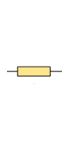
\includegraphics[scale=0.8]{comp.png}
                \captionsetup{justification=centering}
                \caption{Component or combination \\of components}
       \end{subfigure}%
       \begin{subfigure}[t]{0.3\textwidth}
				\centering
                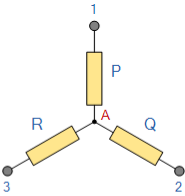
\includegraphics[scale=0.6]{star.png}
                \caption{Star connection}
        \end{subfigure}%
        \begin{subfigure}[t]{0.3\textwidth}
        		\centering
                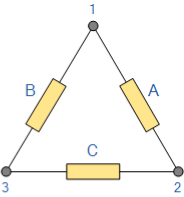
\includegraphics[scale=0.6]{delta.png}
                \caption{Delta connection}
        \end{subfigure}%
        \caption{Circuit connections}
        \label{fig:starAndDelta}
\end{figure}

\begin{figure}[!htb]
\centering
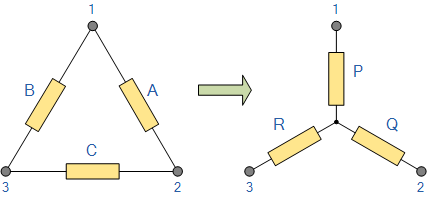
\includegraphics[scale=0.6]{stardelta.png}
\caption{Star to Delta conversion}
\label{fig:starToDelta}
\end{figure}

The following formulae will allow you to move between a star connection and its associated delta connection and vice versa:

\begin{minipage}{0.5\textwidth}
\centering
\paragraph*{Delta to Star Network:}
\begin{equation*}
\begin{aligned}
P &= \frac{A B}{A + B + C}\\
Q &= \frac{A C}{A + B + C}\\
P &= \frac{B C}{A + B + C}\\
\end{aligned}
\end{equation*}
\end{minipage}
\begin{minipage}{0.5\textwidth}
\centering
\paragraph*{Star to Delta Network:}
\begin{equation*}
\begin{aligned}
A &= \frac{P Q + Q R + R P}{R}\\
B &= \frac{P Q + Q R + R P}{Q}\\
C &= \frac{P Q + Q R + R P}{P}\\
\end{aligned}
\end{equation*}

\end{minipage}


\subsection*{Passive circuit components}

Passive circuit components are electrical components that cannot control the current in a circuit. They do not generate power, but instead dissipate, store, and/or release it. Some such components are discussed below.

\subsubsection*{Resistors}

A resistor is a two-terminal passive electronics component used to oppose or limit the current in a circuit. A resistor works based on the principle of Ohm’s law which states that the voltage applied across the terminals of a resistor is directly proportional to the current flowing through it, with the constant of proportionality called the \textit{resistance}.

\begin{equation*}
V = I R
\end{equation*}

\subsubsection*{Capacitors}

A capacitor, made from two conductive plates with an insulator between them, stores electrical energy in the form of an electric field. It blocks the DC signals and allows the AC signals to pass through it. The charge stored in a capacitor is given by

\begin{equation*}
Q = CV
\end{equation*}

When used with a resistor, the time a capacitor takes to charge or discharge is measured in units of an intrinsic time scale, known as the time constant $\tau = RC$ of the circuit.

\subsection*{Active circuit components}
An active device is any type of circuit component with the ability to electrically control electron flow in the circuit.

\subsubsection*{Batteries}

Charges can be separated by several means to produce a voltage. A battery uses a chemical reaction to produce energy and separate opposite sign charges onto its two terminals. As the charge is drawn off by an external circuit, doing work and finally returning to the opposite terminal, more chemicals in the battery react to restore the charge difference and the voltage.


\subsubsection*{p-n junction Diodes}

A p-n junction diode is two-terminal semiconductor device, which allows the electric current in only one direction while blocks the electric current in opposite or reverse direction. Such a diode has an anode (or positive end) containing positive charge carriers called `holes', and a cathode (or negative end) containing negative charge carriers or electrons. The interface between these ends forms a region without any charge carriers called the \textbf{depletion layer}. 

The process of applying the external voltage to a p-n junction semiconductor diode is called biasing. If the diode is \textbf{forward biased} -- that is, when a positive voltage is applied to the anode and a negative voltage to the cathode -- it allows the charge carriers, and hence electric current, to flow. On the other hand, if the diode is \textbf{reverse biased} -- negative to the anode and positive to the cathode -- it blocks the current flow. In the conventional symbol for a diode, the arrowhead indicates the conventional direction of electric current when the diode is forward biased.

Unlike a resistor, a diode does not behave linearly with respect to the applied voltage as the diode has an exponential current-voltage (I-V) relationship and therefore cannot be described by simply using an equation such as Ohm’s law. The basic reason for this is that the width of the depletion layer decreases with increase in positive voltage. After a certain `knee' voltage (0.3 V for Germanium semiconductors and 0.7V for Silicon semiconductors) the width of the barrier effectively goes to zero, and the diode acts like a short circuit with zero resistance. When a junction diode is reverse biased the thickness of the depletion region increases and the diode acts like an open circuit blocking any current flow (except only a very small leakage current), until an `avalanche' voltage when the device overheats and gets shorted leading again to maximum current flow in the opposite direction.

\begin{figure}[!htb]
\centering
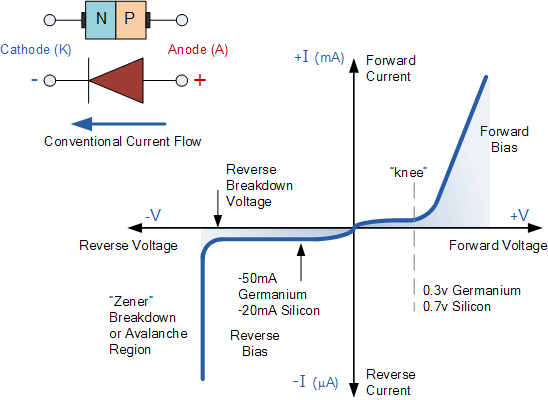
\includegraphics[scale=0.6]{diodeChar.png}
\caption{Diodes and their characteristics}
\label{fig:diodeChar}
\end{figure}



\section*{Experimental Setup}


\subsection*{Black Box}
The black box contains an unknown circuit inside it which is connected to terminals A, B, and C in either a `star' or a `delta' connection (explained above). You have to use these for your analysis and measurements. Do not try to open the given black box.

\subsection*{Digital Multimeter (\textit{MECO 603})}

A multimeter is an instrument used to measure multiple parameters like voltage, current, and resistance. In this experiment you will use the given digital multimeters (Model \textit{MECO - 603}) \textbf{\textit{only}} for the measurement of DC and AC voltage and current. You will have to use input sockets marked COM, V/$\Omega$ and mA (or 20A) for the required measurements. Note that there are two input sockets marked mA and 20A for the current measurement. The socket marked mA may be used for measuring current below 250 mA and socket marked 20A may be used for measuring current up to 20 A. You will have to select the appropriate function and the range using the rotary switch provided on the multimeter. The value of voltage or current is displayed on the LCD screen. The multimeter is turned off by turning the dial to the appropriate setting.

\subsection*{Variable DC Power Supply (\textit{Keltronix})}

The power switch can be used to switch it ON or OFF. The required output can be taken from the two output terminals. The voltage and the current capacity can be changed using the three knobs: voltage coarse, voltage fine, and current. The given power supply also displays the value sof the output voltage and current. Do not use these value since measuring these values using given calibrated multimeter will be more reliable. 

The DC Variable Power Supply can either act as a source of Constant Current (CC) or Constant Voltage (CV), indicated by the two LEDs present on it. In general, most types of circuits require a constant voltage to operate, so if the CV LED is lit, the supply is working fine with your circuit. The power supply has a physical limit on how much current it can supply, if the load (your circuit) attempts to draw more, the power supply decreases the output voltage to keep the current consumed at its maximum permissible amount. For this experiment, you should turn the current dial up to the maximum. This allows the supply to work as a constant voltage supply unless the current drawn by your circuit goes beyond 1A.

\subsection*{Function Generator (\textit{Testronix 72})}

A function generator is a type of signal generator that is used to generate simple repetitive waveforms in the form of an alternating electrical wave. Typically, it will produce waveforms or functions such as sine waves, sawtooth waveforms, square, and triangular waveforms, and will allow you to adjust the frequency and amplitude of  the signals. The instrument given to you generates sine and square waveforms. The output may be taken from the output sockets for the respective waveforms. The frequency can be adjusted by turning the dial and selecting the appropriate Frequency Multiplier button. For example, turning the dial to 3 and selecting the 10k button would provide an output waveform with a frequency of 30kHz. Similarly the amplitude switch, used in conjunction with the appropriate buttons, can be used to adjust the amplitude of the output waveform from under 0V to 30V.



\subsection*{Warnings}

\begin{enumerate}
\item The use of a multimeter to measure the resistance is strictly prohibited.
\item Do not try to open the black box, use only terminals A, B and C for the connections.
\item Use fixed value resistors to prevent large currents in the circuit. The current should not exceed 500 mA.
\item \textbf{Do not} short the outputs of the power supply, it could damage the equipment.
\item Passing more current through the multimeter's (250 mA or 20A) sockets than they can handle will cause the fuses in the multimeter to burn out, leading to an open circuit. Use an appropriate resistance to limit the current in the circuit.
\item When drawing circuit diagrams use the standard symbols.
\item The digital multimeter, the DC power supply or the signal generator should be turned off if not in use.

\end{enumerate}


\section*{Procedural Instructions}

Design the most appropriate method to identify the circuit and determine the values of the electronic components used  in it. Give your answer in the form of a circuit diagram showing the terminals A, B, and C clearly. You will need to give \textit{all} the information required in order to reconstruct the circuit. For example, if you are doing Part A, you will need to determine the values of the resistors, the orientation of the diodes, and the voltage and orientation of the battery, if any of the above are used in the circuit.

In every part, clearly report the procedural steps you have taken with reference to your complete plan of experiment, the data will you collect, how the collected data will be analysed and finally the interpretation of your analysis. Your reporting should be comprehensive, and you are expected to mention all important procedural steps in your answer sheet.



\section*{References}

\begin{enumerate}

\item \href{https://www.elprocus.com/major-electronic-components/}{Overview of Various Basic Electronics Components}

\item \href{https://www.electronics-tutorials.ws/dccircuits/dcp_10.html}{Star Delta Transformation}

\item \href{https://www.electronics-tutorials.ws/diode/diode_3.html}{Electronics Tutorials: PN Junction Diode}

\end{enumerate}


\newpage
% % \title{The Incandescent Lamp and the Inverse Square Law}
% \author{An Introduction to Physics through Experiments}
% \date{}
% \maketitle

\chapter{The Incandescent Lamp and the Inverse Square Law}

\section*{Objectives}

\begin{enumerate}
\item To understand the current-voltage characteristics of an incandescent lamp's filament.
\item To understand the dependence of the lamp's power on the resistance of its filament.
\item To observe and understand the variation of intensity with distance for a point source.
\end{enumerate}




\section*{Apparatus}

\begin{enumerate}
\item A DC variable power supply (\textit{Optochem})
\item Two digital multimeters with probes (\textit{MECO 603} and \textit{Victor VC97})
\item A 12 V, 21W incandescent lamp
\item A stand to hold the lamp
\item A Resistor Ladder
\item Connecting cords
\item A convex lens
\item A photodiode

\end{enumerate}


\section*{Introduction}

All matter that has a temperature greater than absolute zero emits electromagnetic radiation through a process known as thermal radiation. This `heat' represents the conversion of thermal energy into electromagnetic energy. All matter with a temperature by definition is composed of particles which have kinetic energy, and which interact with each other. Thermal energy is a measure of this kinetic energy of random movements of atoms and molecules in matter which are composed of charged particles (protons and electrons), and the kinetic interactions among matter particles result in the emission of photons, radiating energy away from the body through its surface. Such electromagnetic radiation, which includes light, does not require the presence of matter to propagate and travels in the vacuum of space infinitely far if unobstructed.

The characteristics of thermal radiation depend on various properties of the surface it is emanating from, including its temperature. The radiation is not `monochromatic', i.e.\, it does not consist of just a single frequency, but comprises a continuous dispersion energies, known as its characteristic \textit{spectrum}.


An incandescent lamp is composed of a wire filament heated to such a high temperature that it begins to glow with visible light. The filament is protected from oxidation with a glass or fused quartz bulb that is filled with inert gas or a vacuum.



\section*{Description}

In \textbf{Part A}, you will design an experiment to study the VI characteristics of an incandescent lamp. 

In \textbf{Part B}, you will design an experiment to observe the variation of the lamp's power with the resistance of its filament. 

In \textbf{Part C}, you will design an experiment to create a point source and then observe the variation of its intensity as a function of the distance from the source. 


\section*{Theory}

\subsection*{Part A}

If an electric current is passed through a wire of significant resistance, the wire will be heated. If the wire is heated to a sufficiently high temperature, it will give off light.  This is the basis of a resistive incandescent lamp. The high melting point of tungsten (3680 K) and its low vaporization pressure makes it a suitable material to be used as the filament of almost all incandescent lamps. The brightness and the overall colour of emitted light depends on the temperature of the filament for a given lamp, which is a non-linear resistive element.

It is observed that (for a specific range of current) almost all incandescent lamps satisfy the relation

\begin{equation*}
V = K I^a
\end{equation*}

where $V$ is the voltage across the lamp, $I$ the current passing through the lamp, and $K$ and $a$ are constants.

\subsection*{Part B}


One finds for the resistive lamp, the empirical relation

\begin{equation*}
P = C R^n
\end{equation*}

where $P$ is the power supplied to the lamp, $R$ is the resistance of the filament of the lamp, and $n$ and $C$ are constants whose values depend on the material used for the filament of the lamp. The above relation yields better results when the temperature of the filament of the lamp is approximately above 1800 K for the given lamp. For such temperatures the resistance R of the lamp is found to be directly proportional to the absolute temperature T of the filament of the lamp.



\subsection*{Part C}


\begin{minipage}{0.5\linewidth}
%\vspace{-1.5cm}
A \textbf{point source} is a single identifiable localised source of, say, light. Such a source has negligible extent, distinguishing it from other source geometries, and are called point sources because in mathematical modelling, they can usually be approximated as a mathematical point to simplify analysis. The actual source need not be physically small, if its size is negligible relative to other length scales in the problem. For example, in astronomy, stars are routinely treated as point sources, even though they are in actuality much larger than the Earth.~\\

For light or sound waves, a point source radiates the same intensity of radiation in all directions. That is, it has no preferred direction of radiation and radiates uniformly in all directions over a sphere centred on the source.
\end{minipage}
\begin{minipage}{0.5\linewidth}
\centering
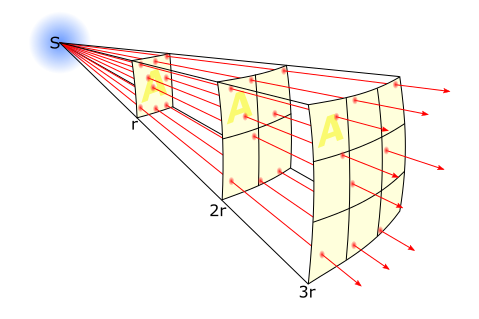
\includegraphics[scale=0.7]{isl.png}
\end{minipage}



\section*{Experimental Setup}

\subsection*{Digital Multimeter (\textit{MECO 603})}

A multimeter is an instrument used to measure multiple parameters like voltage, current, and resistance. In this experiment you are given two digital multimeters (Models \textit{MECO - 603} and \textit{Victor VC97})\footnote{The Victor multimeter has a greater current sensitivity.}. You will have to use input sockets marked COM, V/$\Omega$ and mA (or A or 20A) for the required measurements. Note that there are two input sockets marked mA and 20A (10A for the Victor multimeter) for the current measurement. The socket marked mA may be used for measuring current below 250 mA and socket marked 20A (or 10A) may be used for measuring current up to 20 A (or 10A). You will have to select the appropriate function and the range using the rotary switch provided on the multimeter. The value of voltage or current is displayed on the LCD screen. The multimeter is turned off by turning the dial to the appropriate setting.

\subsection*{Variable DC Power Supply (\textit{Optochem})}

The power switch can be used to switch it ON or OFF. The required output can be taken from the two output terminals. The voltage and the current capacity can be changed using the three knobs: voltage coarse, voltage fine, and current. The given power supply also displays the values of the output voltage and current. Do not use these value since measuring these values using given calibrated multimeter will be more reliable. 

The DC Variable Power Supply can either act as a source of Constant Current (CC) or Constant Voltage (CV). In general, most types of circuits require a constant voltage to operate. The power supply has a physical limit on how much current it can supply, if the load (your circuit) attempts to draw more, the power supply decreases the output voltage to keep the current consumed at its maximum permissible amount. For this experiment, you should turn the current dial up to the maximum. This allows the supply to work as a constant voltage supply unless the current drawn by your circuit goes beyond 2A.

\subsection*{Photodiode}

A photodiode is a semiconductor device that converts light into an electrical current. The current is generated when photons of sufficient energy are absorbed in the photodiode, creating an electron-hole pair through the photoelectric effect.

\subsection*{Warnings}

\begin{enumerate}
\item Do not apply a voltage more than 12 V to the lamp.
\item Clamp the lamp carefully on the retort stand so that the wires do not get shorted accidentally.
\item You will have to use the given fixed value resistor to control the current in the circuit.
\item Use the digital multimeter for the measurement of DC voltage and current.  Choose the appropriate range for the measurement.
\item The incandescent lamp should not be kept connected to the power supply for long duration. 

\item Passing more current through the multimeter's (250 mA or 20A) sockets than they can handle will cause the fuses in the multimeter to burn out, leading to an open circuit. Use an appropriate resistance to limit the current in the circuit.

\item When drawing circuit diagrams use the standard symbols.

\item The digital multimeter and the DC power supply should be turned off if not in use.

\end{enumerate}


\section*{Procedural Instructions}

\subsection*{Part A}

You have to design and perform an experiment to determine the value of constant a for the given incandescent lamp, given that it follows the equation 

\begin{equation*}
V = K I^a
\end{equation*}

You will have to plot an appropriate graph and from the graph determine the value of $a$. Draw the necessary circuit diagram in your answer sheet.

\begin{question}
\paragraph{Question:} Describe qualitatively how you would expect the resistance of the lamp to vary with the current. Explain why you think this is the case.
\end{question}

\subsection*{Part B}

You have to design an appropriate procedure to determine the value of $n$. You may use the data gathered earlier, or you may perform new measurements. Plot the appropriate graph to determine the value of $n$.

\subsection*{Part C}

In this part, you have to study the fall of intensity of light emitted by the given incandescent lamp.  For this you have to use the given photodiode with a digital multimeter to measure the intensity of light. We assume that the relation between the intensity of light incident on the sensing area of the photodiode and its output current is linear. 

Use the converging lens that we have provided you with in order to create a point source. You may use the screen with a hole in it to allow the passage of a small amount of light of this `point source' that may then be detected by the photodiode. This screen will now act as your source.

Connect the output of the power supply to the given lamp and adjust the voltage applied to the lamp to be around 12 V. Keep the photodiode initially as close as possible to the screen acting as your source.  Study the variation of current IPD in the photodiode with the distance $d$ between the source and the photodiode. (You have to take readings for the value of $d$ varying from around 7.0 cm to around 50.0 cm.) You may have to correct your readings to account for the ambient light falling on the photodiode. 

Plot an appropriate linear graph to show the variation of the intensity of light with distance $d$.

\begin{question}
\paragraph{Question:} What type of graph would be the most efficient to determine the variation of the intensity of light with distance? Why? ~\\

\paragraph{Question:} After plotting this graph, you may find that points below a certain value (say, 20.0 cm) do not behave as you would expect them to. Can you explain why this is the case?
\end{question}


\section*{References}

\begin{enumerate}

\item \href{https://www.fh-muenster.de/ciw/downloads/personal/juestel/juestel/4-InkohaerenteLichtquellen-Glueh-_und_Halogenlampen_english_-1.pdf}{Incandescent and Halogen Lamps}

\item \href{https://www.elprocus.com/photodiode-working-principle-applications/}{Photodiode Working Principle, Characteristics and Applications}

\end{enumerate}



\newpage
% % \title{Diffraction of Light}
% \author{An Introduction to Physics through Experiments}
% \date{}
% \maketitle

\chapter{Diffraction of Light}

\section*{Objectives}

\begin{enumerate}
    \item To determine the wavelength $\lambda$ of the light emitted by a laser source by studying the diffraction of light due to plane diffraction gratings.
    \item To determine the width of the given single slit by studying its diffraction pattern.
    \item To determine the diameter of a given wire by studying its diffraction pattern.
    \item To determine the size of the circular aperture by studying its diffraction pattern.
\end{enumerate}



\section*{Apparatus}

\begin{enumerate}
    \item A 10 mW semiconductor red laser source.
    \item A 5 mW DPSS green laser source.
    \item A set of necessary mounts.
    \item A set of plane diffraction gratings of different grating spacings.
    \item A single helix (spring) set in a holder
    \item A double helix set in a holder
    \item Measuring tapes.
    \item A holder for grating.
    \item A set of screens.  
    \item A single slit of fixed width mounted on a slide.
    \item Two multiple slits mounted on slides.
    \item Circular apertures mounted on slides.
    \item A spirit level
\end{enumerate}

\section*{Introduction}
	 
In \textit{Opticks} (1704), Issac Newton wrote, ``Light is never known to follow crooked passages nor to bend into the shadow''. He explained this by describing how particles of light always travel in a straight line, and how objects kept in the path of the light cast a shadow because the particles can never spread out behind the object. However, a set of experiments on the propagation of light through small apertures performed by Francesco Grimaldi, Augustine Fresnel, Thomas Young and a few others firmly established that light actually enters into the shadow region with a definite pattern when it passes through around an edge. The resulting pattern depends on the relative size of the aperture or obstacle and the wavelength of light. If the size is much larger than the wavelength, the bending will be almost unnoticeable. However, if the two are similar in size, the diffraction will be considerable.    
     
In this experimental problem, we will use a low power solid-state laser as a source of an intense beam of monochromatic light. When light from a distant source (or a laser source) passes around a thin aperture or through a narrow aperture and is then intercepted by a viewing screen, the light produces a pattern on the screen called a \textit{diffraction pattern}. When such a beam is incident on various diffracting components like a plane diffraction grating, a single slit, a wire mesh or a two-dimensional diffraction grating, the light emerging from these components show a variety of interesting diffraction patterns. This pattern consists regions of maximum and minimum intensities, which characterise the diffracting object. 

\section*{Theory}


\begin{imp}

\begin{center}
    \textbf{Babinet's Principle}
\end{center}

Two objects are called \textit{complementary} if one of them is transparent where the other is opaque and opaque where the other is transparent. An example of this is given in Figure (\ref{fig:complementary}).~\\

\textbf{Babinet's principle} states that

\begin{center}
``Complementary objects \textbf{produce the same diffraction pattern}, except for the intensity of the central maxima.''
\end{center}

This is a highly non-intuitive result, and one that you may study in some of your later courses. The mathematics of this are far beyond the scope of this lab session. 
Henceforth we will not differentiate between the patterns made by such complementary objects. We will thus speak of a single slit (or of a thin wire) having the `same' diffraction pattern, keeping in mind that the intensities of the central maxima are different.
\end{imp}

\begin{figure}[!htb]
    \centering
    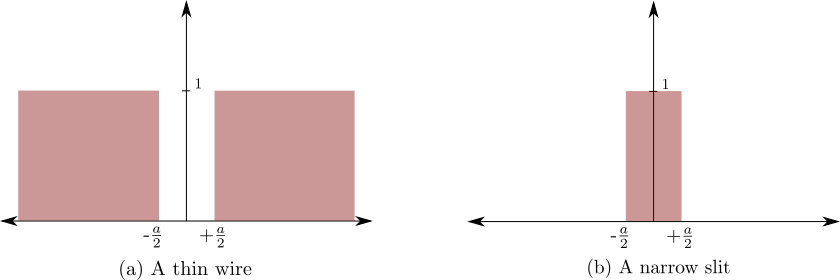
\includegraphics[scale=0.6]{figs/complementary.png}
    \caption{Transparency of a thin wire and of a single slit.}
    \label{fig:complementary}
\end{figure}

\begin{question}
\paragraph{Question:} What are the complementary objects of the following:

\begin{enumerate}
\item A transparent sheet of paper.
\item A circular aperture of diameter $d$.
\end{enumerate}
\end{question}



\subsection*{The Single Slit (or Thin Wire)}

When a (monochromatic) beam of light such as a laser is incident on a narrow single slit, the light emerging from the slit shows a diffraction pattern on a screen. The distribution of the intensity of light received on a screen show a pattern of varying intensity consisting of a bright central maximum with alternate minima and maxima of decreasing intensity on either side, known as a \textit{Fraunhofer diffraction pattern}.

Similarly, instead of a slit of width $a$, supposing we had a \textit{wire} of diameter $a$ placed as an obstruction to the laser beam. The resulting intensity pattern as observed on a screen almost exactly the same as that observed for a single slit. This intensity distribution can be written as a function of the angle $\theta$ as

\begin{equation*}
    I(\theta) = I(0) \left( \frac{\sin \beta}{\beta} \right)^2, \quad \quad  \beta = \frac{\pi a \sin \theta}{\lambda}
\end{equation*}

This function has been represented in Figure (\ref{fig:singleslit}).

\begin{figure}[!htb]
    \centering
    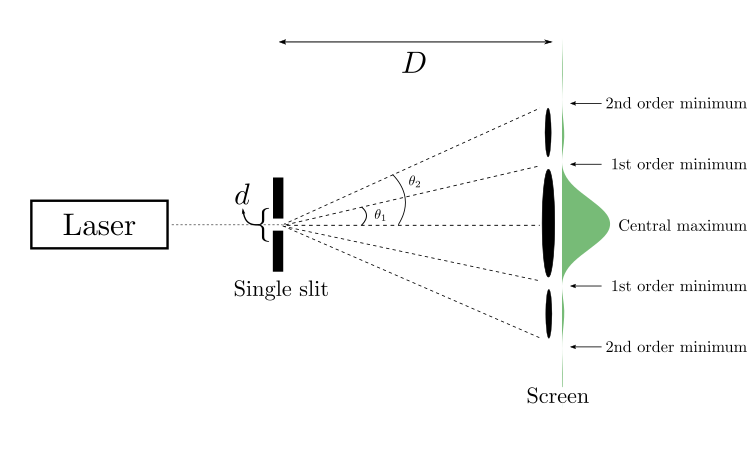
\includegraphics[width=0.75\textwidth]{figs/singleslit.png}
    \caption{The diffraction pattern produced by a single-slit aperture (or thin wire).}
    \label{fig:singleslit}
\end{figure}


Moving away from the central spot, when $\sin\beta=0$ (but $\beta \neq 0$), the intensity vanishes! The positions of these \textbf{minima} (zeros) of the intensity distribution pattern are given by the relation 

\begin{equation}
   a \sin{\theta_m} = \pm m \lambda  \quad\quad\quad \text{for    m  = 1, 2, 3,}\hdots,
   \label{singleslit}
\end{equation}

where $\lambda$ is the wavelength of the incident light, $a$ is the width of the slit and $\theta_m$ is the angle corresponding to $m$th minimum. Here the $\pm$ refers to either side of the central spot ($\theta = 0$).


\subsection*{The Double Slit}

We can now imagine two single slits of the same width next to each other. Such an arrangement is called a double-slit aperture. We could think of this aperture (shown in Figure (\ref{fig:doubleslit})) as a combination of a single slit of width $d$, and a thin wire of width $a$. 

This situation is slightly more complicated than the previous one; the thin obstacle of width $a$ will produce a diffraction pattern like the one in the previous section. However, the light from the two slits on either side will \textbf{interfere}, producing an overall interference pattern which also has its own maxima and minima! The mathematics of this is too difficult to understand right now; you will cover it in a later laboratory.

The resultant intensity distribution is given by   

\begin{equation}
    I(\theta) = I(0) \cos^2\delta \left( \frac{\sin \beta}{\beta} \right)^2, \quad \quad  \beta = \frac{\pi a \sin \theta}{\lambda}, \quad \delta = \frac{\pi d \sin \theta}{\lambda}
\end{equation}

For a screen placed at a large distance $D$ from the wire, the positions of the minima on the screen are observed at 

\begin{equation}
    \begin{aligned}
        x_{\pm n} = \pm n \frac{\lambda D}{a}, &\quad& \text{due to diffraction},\\
        x_{\pm m} = \pm \left( m - \frac{1}{2}\right) \frac{\lambda D}{d}, &\quad& \text{due to interference}
    \end{aligned}
    \label{doubleslit}
\end{equation}


\begin{figure}[!htb]
    \centering
    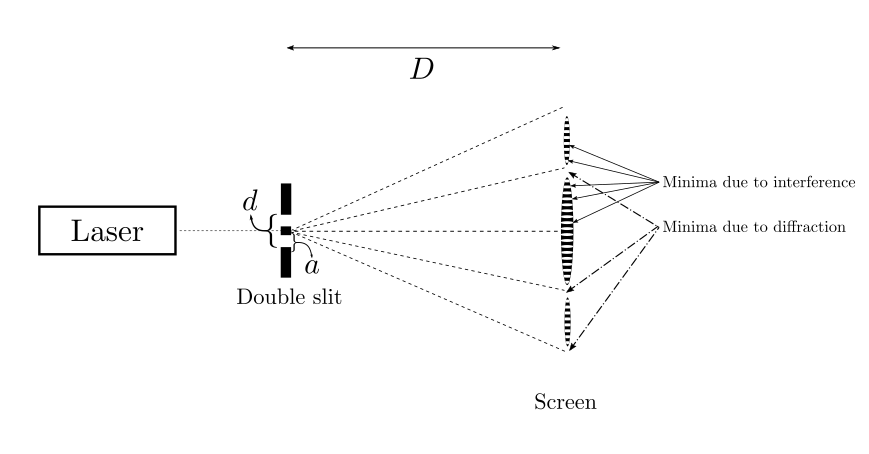
\includegraphics[width=0.75\textwidth]{figs/doubleslit.png}
    \caption{The diffraction pattern produced by a double-slit aperture is a combination of two patterns (diffraction due to a single wire and interference due to two slits).}
    \label{fig:doubleslit}
\end{figure}



\begin{question}
\paragraph{Question:} Look at the above condition for the fringes produced due to diffraction in Equation (\ref{doubleslit}). Is it different from the result obtained in the previous section (Equation (\ref{singleslit}))? If yes, why? If no, why not?~\\
\paragraph{Question:} What is the ``complementary'' object to a double-slit?
\end{question}



\subsection*{Plane Diffraction Grating}

A transmission diffraction grating consists of a large number of slits separated from one another by an opaque region. The grating concentrates the diffracted light along a particular direction in contrast to the single slit, which has a rather broad diffraction maximum. The maxima (bright intense spots) produced by a grating are usually called the principal maxima. They are quite intense and are also widely separated; what cannot be detected visually are the large number of secondary maxima which lie between neighbouring principal maxima.

The expression, relating wavelength $\lambda$ of light used and the grating spacing $d$, with angle of deviation $\theta$ is
\begin{equation*}
    d \sin{\theta_m} = m \lambda,  \quad\quad\quad \text{for    m  = 1, 2, 3,}\hdots
\end{equation*}

In the above expression, $m$ represents the order of \textbf{maxima} points and the angle $\theta_m$  corresponds to  $m$th  order maximum intensity point. This relation is valid for a single slit and for the wire-like obstacle.

\begin{figure}[!htb]
    \centering
    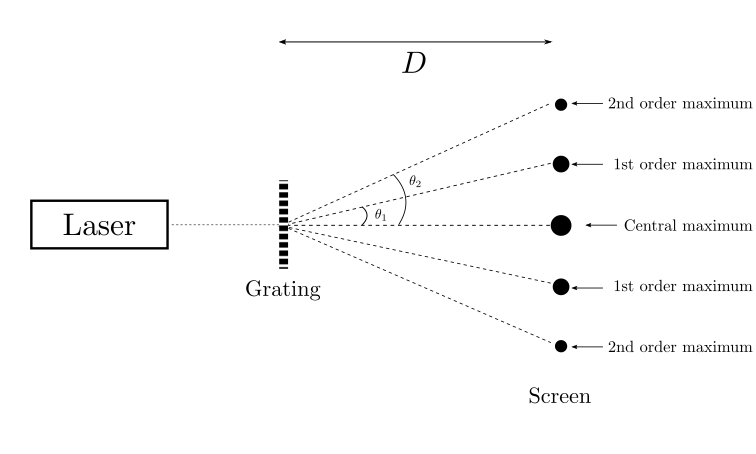
\includegraphics[width=0.75\textwidth]{figs/grating.png}
    \caption{The diffraction pattern produced by a plane diffraction grating.}
    \label{fig:grating}
\end{figure}


\subsection*{The Circular Aperture}

The diffraction pattern due to a circular aperture (known as an \textit{Airy diffraction pattern}) is similar to a single slit diffraction but the mathematics involved is more complicated which gives the expression nearly identical to that of the single slit. Hence we may apply the same expression to the diffraction due to a circular aperture, 

\begin{equation*}
    d \sin{\theta_m} = \overline{m} \lambda,  \quad\quad\quad \text{for    m  = 1, 2, 3,}\hdots
\end{equation*}

where $d$ is the diameter of the circular aperture and $\theta_m$ is the angle of deviation for the $m$th dark ring. The variable $\overline{m}$ has the following values:

\begin{equation*}
    \begin{aligned}
        m = 1 &\quad& \overline{m}=1.22\\
        m = 2 &\quad& \overline{m}=2.23\\
        m = 3 &\quad& \overline{m}=3.23\\
        m = 4 &\quad& \overline{m}=4.24\\
    \end{aligned}
\end{equation*}

\subsection*{Single and double helices:}
  
\begin{figure}[!htb]
    \centering
    \begin{subfigure}[b]{0.45\textwidth}
                \centering
                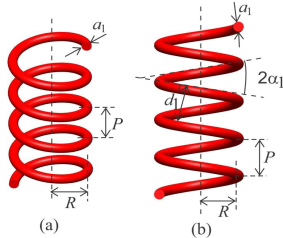
\includegraphics[width=0.75\textwidth]{figs/singlehelix.png}
                \caption{Schematic of a single helix (like RNA)}
                \label{fig:singlehelix1}
        \end{subfigure}%
        \begin{subfigure}[b]{0.45\textwidth}
                \centering
                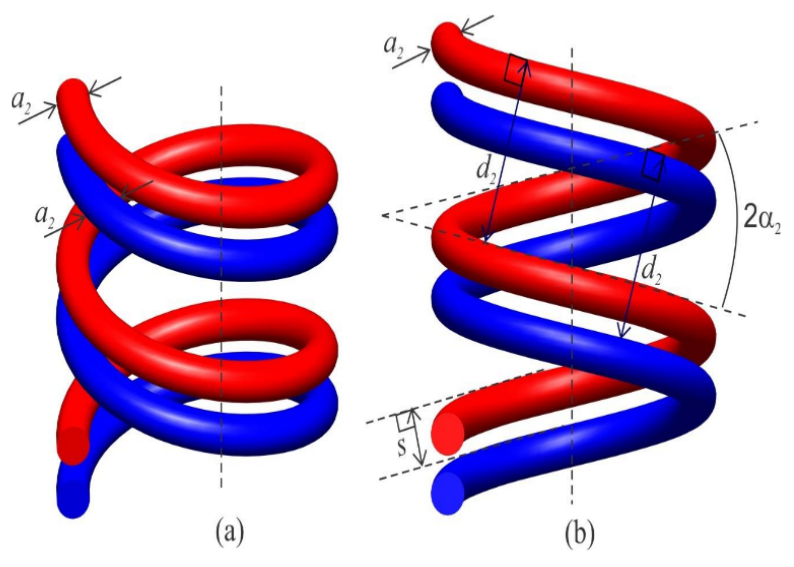
\includegraphics[width=0.75\textwidth]{figs/doublehelix.png}
                \caption{Schematic of a double helix (like DNA)}
                \label{fig:doublehelix1}
        \end{subfigure}
\end{figure}

Now consider a set of four identical wires, the net intensity distribution is a combination of diffraction from each wire and interference due to pairs of wires and hence depends on $a$, $d$ and $s$ (see Figure \ref{fig:fourwires}).

In other words, the combination of three different intensity patterns is observed.

\begin{figure}[!htb]
    \centering
    \begin{subfigure}[b]{0.45\textwidth}
                \centering
                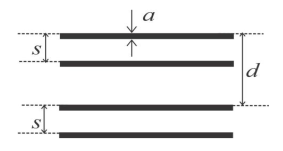
\includegraphics[width=0.75\textwidth]{figs/fourwires.png}
                \caption{Projection of four identical wires}
                \label{fig:fourwires}
        \end{subfigure}%
        \begin{subfigure}[b]{0.45\textwidth}
                \centering
                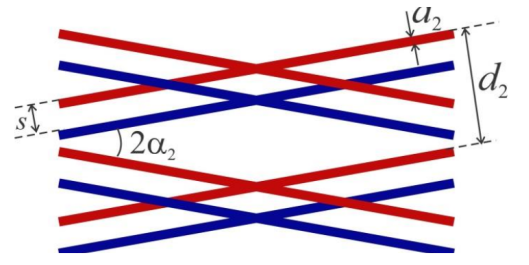
\includegraphics[width=0.75\textwidth]{figs/doublehelix-schema.png}
                \caption{The double helix given in the sample.}
                \label{fig:doublehelix2}
        \end{subfigure}
        \caption{Diffraction patterns of obstacles with three length scales.}
\end{figure}

\section*{Description}

In \textbf{Part A}, you will determine the wavelength of light of a laser using a set of diffraction gratings.

In \textbf{Part B}, you will use the laser whose wavelength you have just determined to measure the width of a single slit.

In \textbf{Part C}, you will study diffraction pattern of a circular aperture.

In \textbf{Part D (\textit{optional})}, you will study the diffraction pattern of a single helix.

In \textbf{Part E (\textit{optional})}, you will study the diffraction pattern of a double helix.


\section*{Procedural Instructions}

\subsection*{Part A}

Observe effect of colour and also of white light on the diffraction pattern obtained by a suitable grating. Then choose an appropriate diffraction grating and perform the measurements to determine the wavelength $\lambda$ of the laser. 

\begin{question}
\paragraph{Question:} Estimate the error in the value of the wavelength of light.~\\

\paragraph{Question:} What are the sources of error in the above-determined value of $\lambda$? What measures should be taken to minimise these errors? ~\\

\paragraph{Question:} Tilt the grating at an angle. How does this affect the diffraction pattern?
\end{question}

Now repeat this procedure for different gratings (with different values of $d$), and calculate wavelength $\lambda$ as accurately as possible.

\subsection*{Part B}

Design and perform the necessary experiment with a single slit of fixed width and determine the width d of the given single slit.

\begin{question}
\paragraph{Question:} Tilt the slit at an angle. How does this affect the diffraction pattern?
\end{question}


\subsection*{Part C}

Now take the given circular aperture as the diffracting object and determine the diameter of the circular aperture.

\subsection*{Part D}

Study of the diffraction pattern due to a helical spring and determine pitch of the spring and thickness of its wire. 


\begin{question}
\paragraph{Question:} Can you explain the form of the diffraction pattern observed? Does this part of the experiment relate in any way to Part B? 
\end{question}

\subsection*{Part E}

Study of the diffraction pattern due to a double helix (as in our DNA) and determine all its parameters, as shown in Figure (\ref{fig:doublehelix2}).

\begin{question}
\paragraph{Question} Describe the diffraction pattern obtained if you use a laser source to illuminate
\begin{enumerate}[label=(\alph*)]
    \itemsep0em
    \item A fine wire mesh,
    \item A square aperture,
    \item A rectangular aperture.
\end{enumerate}
\end{question}



\subsection*{Precautions}

\begin{enumerate}
    \item Never look directly at a laser beam with the naked eye. It may damage the eye permanently.
    \item Never point the laser at anyone else, for the same reason.
    \item Never point an optical device at a laser beam. It could damage the internal sensors.
    \item Never place highly reflective objects (such as rings, watches, and glassware) in the path of the laser beam.
    \item For proper working of laser, it should be kept on throughout. Do not put it off until you complete all your readings, but if you do not need the laser beam for measurements or alignment, use a light-blocking screen to block the  beam.
    \item Treat the laser source as you would any other electrical device: It should never be tampered with while the power cord is connected.
\end{enumerate}


\section*{References}

\begin{enumerate}
\itemsep0em
    \item Eric Stanley, Am. J. Phys., Vol.- 54, No.-10, October 1986, pp. 952.
    \item F.A. Jenkins, H.E. White, \textit{Fundamentals of Optics}, Third Edition, Mc-Graw Hill Kogakusha Ltd., Toyko, Japan, 1957, pp. 288-309, 328-350.
    \item F.W. Sears, \textit{Optics}, Third Edition, Asia Publishing House, 1958, pp 221-252.
    \item R.W. Ditchburn, \textit{Light}, Second Edition, The English Language Book Society and Blackie \& Son Ltd., 1963, pp 162-237.
    \item John Beynon, \textit{Introductory University Optics}, Prentice-Hall of India Pvt. Ltd., New Delhi (India), 1998, pp 158-190.
    \item Rajpal S. Sirohi, \textit{Wave Optics and its Applications}, Orient Longman Limited, (India), 1993, pp 169-210.
\end{enumerate}



\newpage
\begin{refsection}
\chapter{Formation of Rainbow}

\section*{Objectives}

\begin{enumerate}
\item To study different orders of rainbows formed by a drop of water.
\item To study specifically the second-order rainbows for liquids of different refractive indices.
\item To determine the refractive index of an unknown liquid using the second-order rainbow it forms.
\end{enumerate}


\section*{Introduction}
The rainbow is probably one of the most spectacular light shows observed naturally in the sky. The conventional explanation to the formation of a rainbow is that sunlight -- which is composed of a spectrum of colours -- is separated into its constituent colours by the large number of water droplets present in the air on a rainy day, very much like the dispersion of light by a prism. 

However, as we shall see, this is not the full story. To completely understand the formation of the rainbow and its location in the sky, we need to take into account the fact that the droplets are actually spherical, and that the incident light may be reflected many times within the drop before exiting it.

In the case of a primary (or first order) rainbow, the sunlight incident on a raindrop is refracted at the front surface, reflected at the back surface and refracted again as it emerges into the air. 

However, it is possible for sunlight to be reflected internally twice, before exiting the drop. While the intensities of such light rays will be much weaker than those that have been reflected only once, it is possible to see such `secondary' (or higher-order) rainbows in nature. Secondary rainbows -- as we shall see -- are formed at angles that are further out from their primary counterparts. Thus, we speak of the ``order'' of a rainbow as the number of times light has been reflected within the drop.\footnote{\textbf{Note:} While the light \textit{is} reflected inside the drop, it is \textit{not} due to total internal reflection. The angles that the rays of light make with the normal inside the drop are less than the critical angle for the water-air interface.} Higher-order rainbows are almost never seen naturally, as they are weaker than the background brightness of the sky and are usually positioned inconveniently with respect to the sun; if you are lucky, you can sometimes see a second-order rainbow. 

An instructive way to understand the formation of rainbows is to actually study the dispersion of white light by a spherical drop of water, as we shall in the present problem. (Note, however, that we use the word ``rainbow'' very loosely, to mean a ``rainbow-like \textit{spectrum}'' rather than the more familiar ``rainbow'' in the sky.) 


\section*{Theory}

We will be dealing with the propagation of light between different transparent materials. When light moves from one medium to another, it changes direction through a process known as \textit{refraction}. Thus, at least for the purposes of this experiment, we can characterise different transparent media by their refractive indices: a dimensionless number ($\mu$) which describes how much light bends when it enters the medium from vacuum. 

\begin{figure}[!htb]
\captionsetup[subfigure]{justification=centering}
\centering
        \begin{subfigure}[b]{0.5\textwidth}
        \centering
                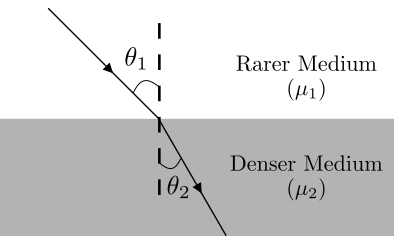
\includegraphics[scale=0.5]{figs/snell1.png}
                \caption{$\mu_1<\mu_2:$\\ The refracted ray is deviated towards normal.}
                \label{fig:rareToDense}
        \end{subfigure}\hfill
        \begin{subfigure}[b]{0.5\textwidth}
        \centering
                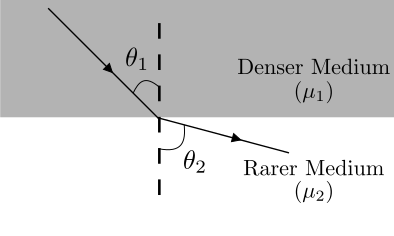
\includegraphics[scale=0.5]{figs/snell2.png}
                \caption{$\mu_1>\mu_2:$\\ The refracted ray is deviated away from normal.}
                \label{fig:denseToRare}
        \end{subfigure}
        \par\bigskip
        % \begin{subfigure}[b]{\textwidth}
        % \centering               
        %         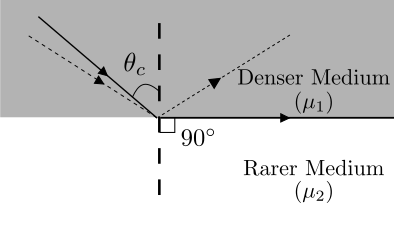
\includegraphics[scale=0.5]{figs/snell3.png}
        %         \caption{$\mu_1>\mu_2:$\\ Beyond some $\theta_c$, the refracted ray is reflected internally.}
        %         \label{fig:til}
        % \end{subfigure}
        \caption{The propagation of a ray of light between media of different refractive indices.}\label{fig:snells}
\end{figure}


The relationships between the angles $\theta_1$ and $\theta_2$ (shown in Figure (\ref{fig:snells})) is given by the Sahl-Snell–Descartes law (usually called Snell's law):

 \begin{equation}
    \mu_1 \sin{\theta_1}= \mu_2 \sin{\theta_2}.
    \label{snell}
 \end{equation}

As light passes from a rarer to a denser medium (as shown in Figure (\ref{fig:rareToDense})), the ray of light bends \textit{towards} the normal, while as light travels from a denser to a rarer medium (Figure (\ref{fig:denseToRare})), the ray of light bends \textit{away} from the normal. 
%When light moves from a denser to a rarer medium ($\mu_1>\mu_2>1$), there must be \textit{some} angle (let's call it $\theta_c$) greater than which the resulting refracted ray bends back inwards (Figure (\ref{fig:til})). This phenomenon, called \textbf{Total Internal Reflection}, plays a crucial role in the formation of the rainbow.



\subsection*{The Primary Rainbow}

Consider Figure (\ref{fig:firstOrder}) for first order $(K = 1)$ rainbow formed by a spherical drop of liquid with refractive index $\mu$.

\begin{figure}[!htb]
    \centering
    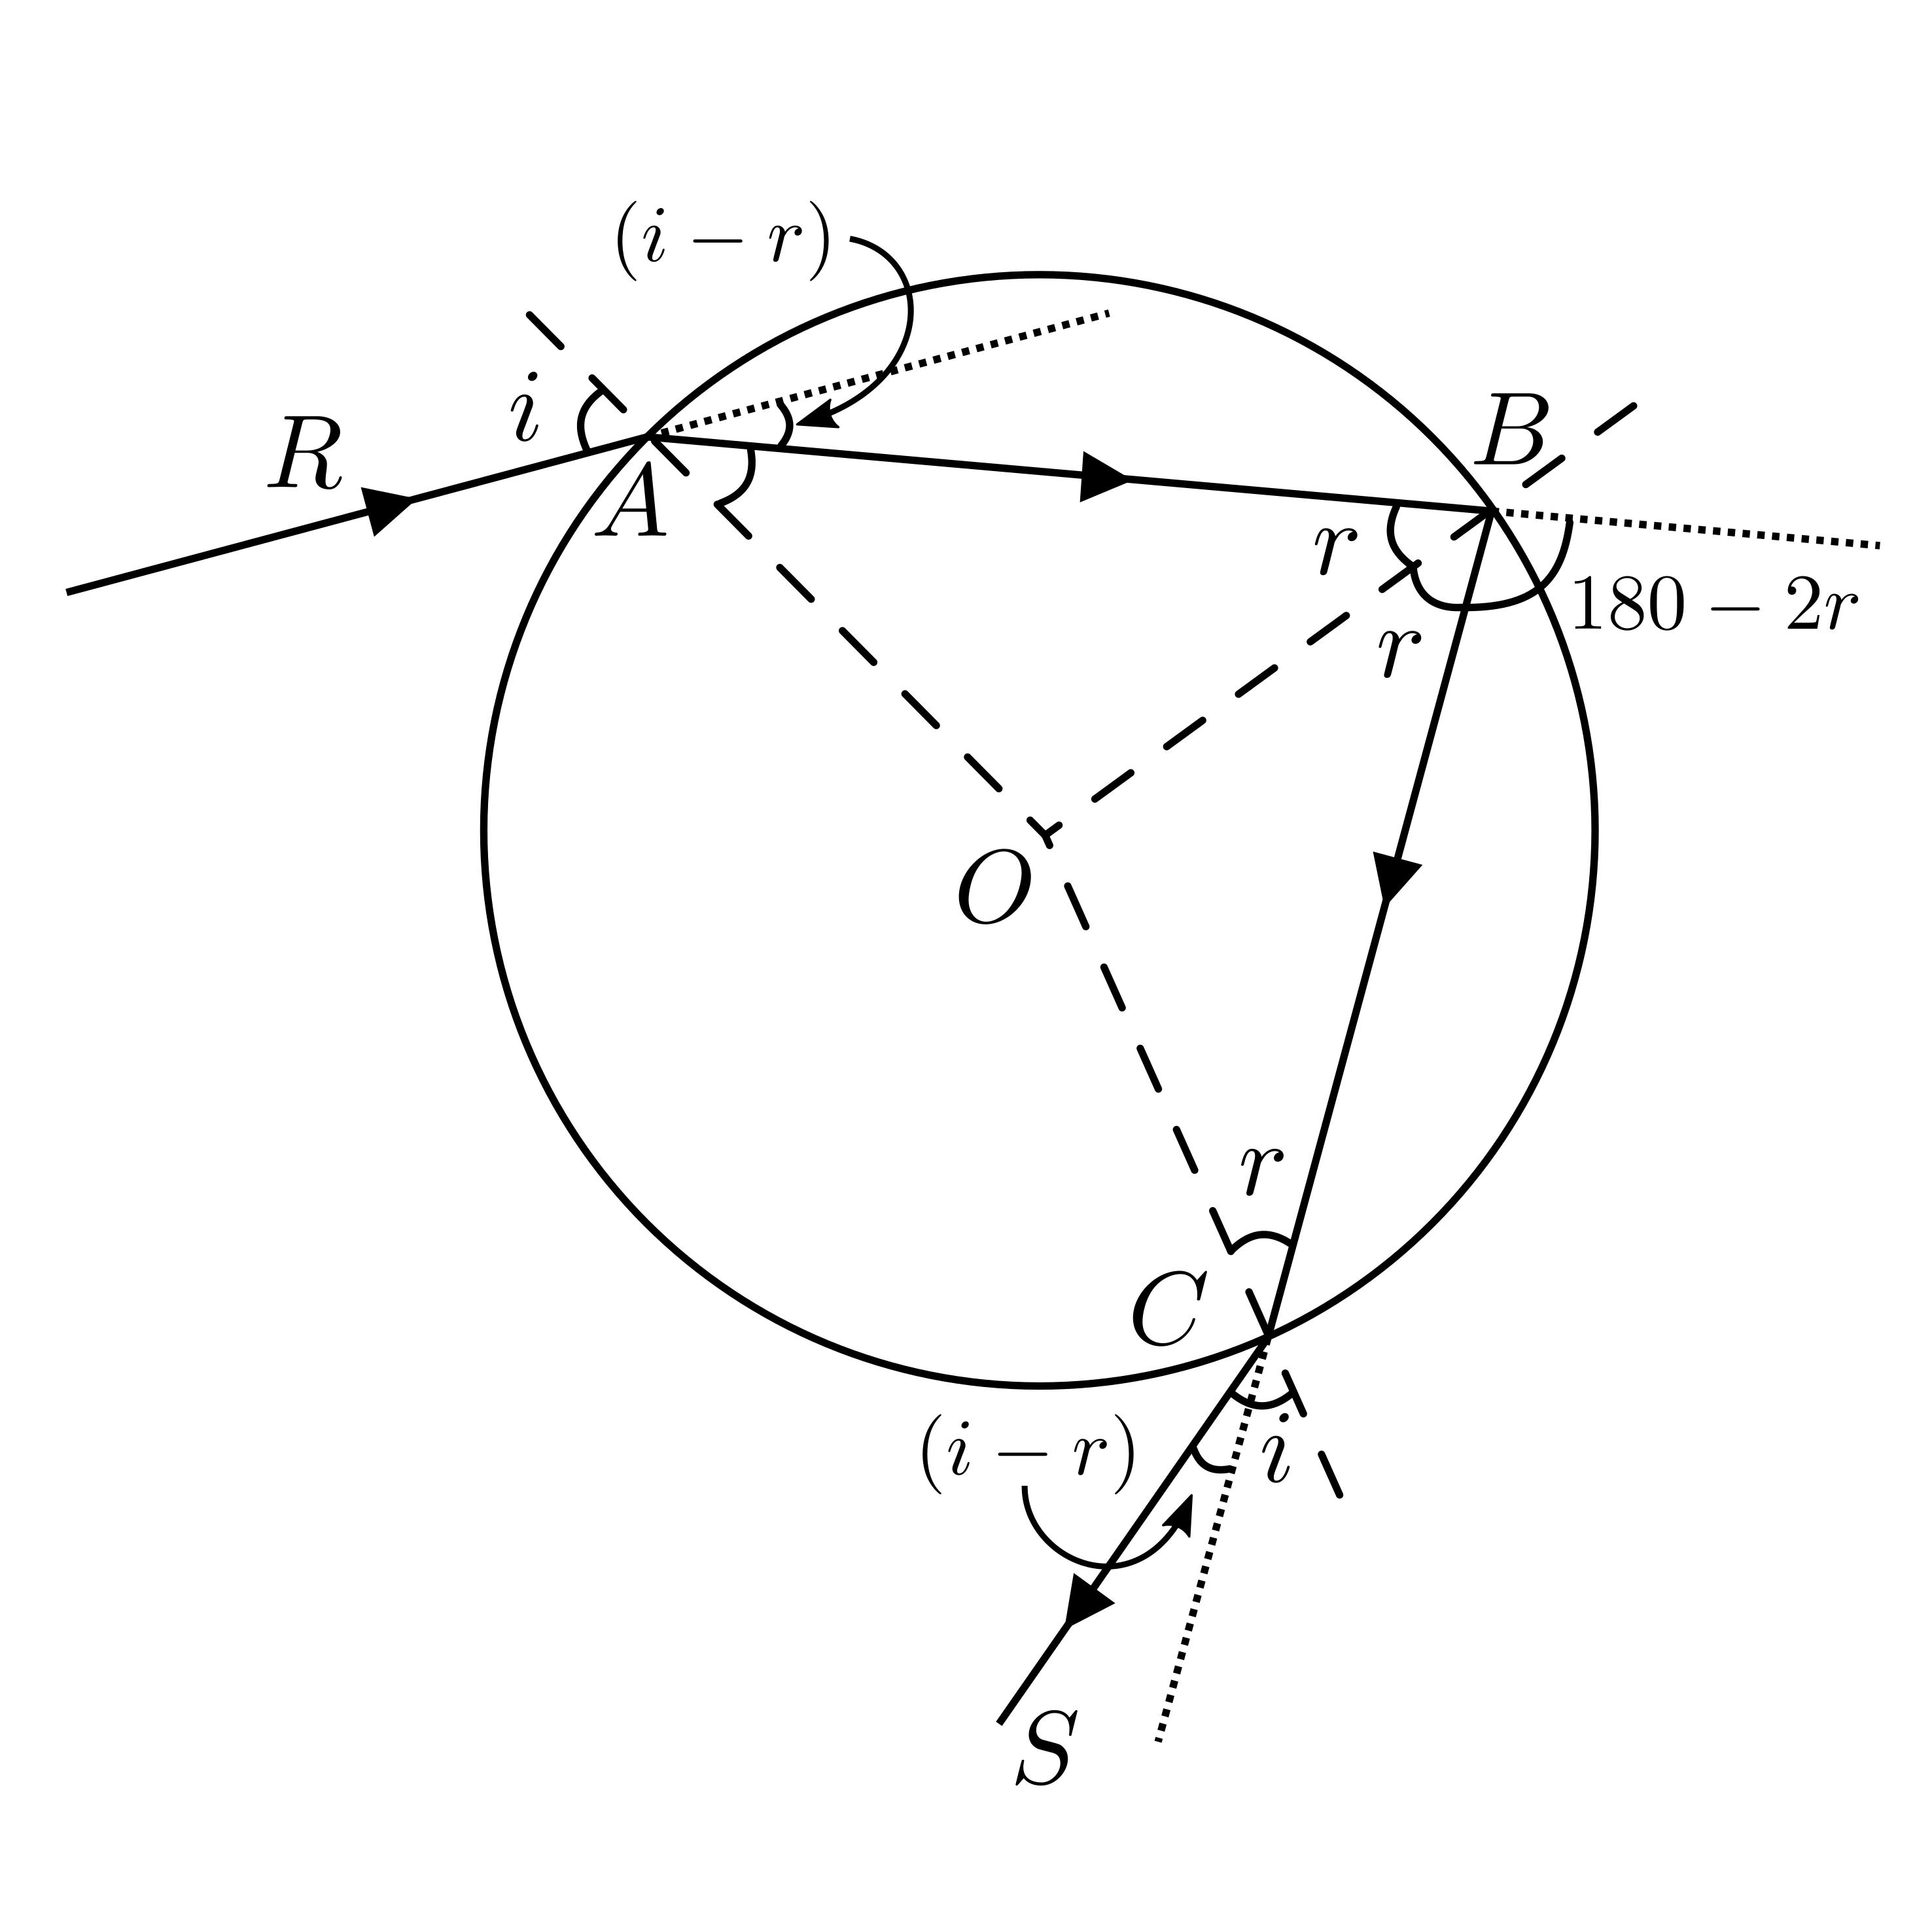
\includegraphics[width=0.5\textwidth]{figs/rainbow1.png}
    \caption{Ray diagram for the formation of a first order rainbow, with angles marked.}
    \label{fig:firstOrder}
\end{figure}


Let $RABCS$ be the path of a ray of incident monochromatic light, which comes out of a spherical droplet of liquid after suffering two refractions at $A$ and $C$ and one reflection at $B$.

Let $i$ be the angle of incidence and $r$ be the angle of refraction at $A$. It should be clear to you that $r$ is also the angle of incidence and reflection at $B$.\footnote{The triangle $ABO$ is an isosceles triangle.} At the point $C$, since the angle of incidence inside the droplet is $r$, the angle of emergence (at $C$) will be $i$. 

\begin{question}
\paragraph{Question:} Show that at the point $C$, the angle of incidence is $r$ and, using Equation (\ref{snell}), that the angle of emergence is indeed $i$.
\end{question}

We can now calculate the total \textit{deviation} of the ray as it passes through the drop. From Figure (\ref{fig:firstOrder}) it should be clear that at the point $A$, if not for the drop the ray would have travelled along the dotted line. Thus, the deviation is $(i-r)$. Similarly, upon reflection at $B$, the ray deviates by $(180-2r)$. And finally, at $C$, the ray again deviates by $(i-r)$. Thus, the total deviation is:

\begin{equation}
\phi_{1}=2(i-r)+(180-2r).
\end{equation}


If we now consider the second-order rainbow as shown in Figure (\ref{fig:secondOrder}). The difference between this case and the previous one is that there are now two reflections within the drop. The deviations due to each of the reflections will be the same, and thus the total deviation due to both the reflections is $2\times (180 - 2r)$. 


\begin{figure}[!htb]
    \centering
    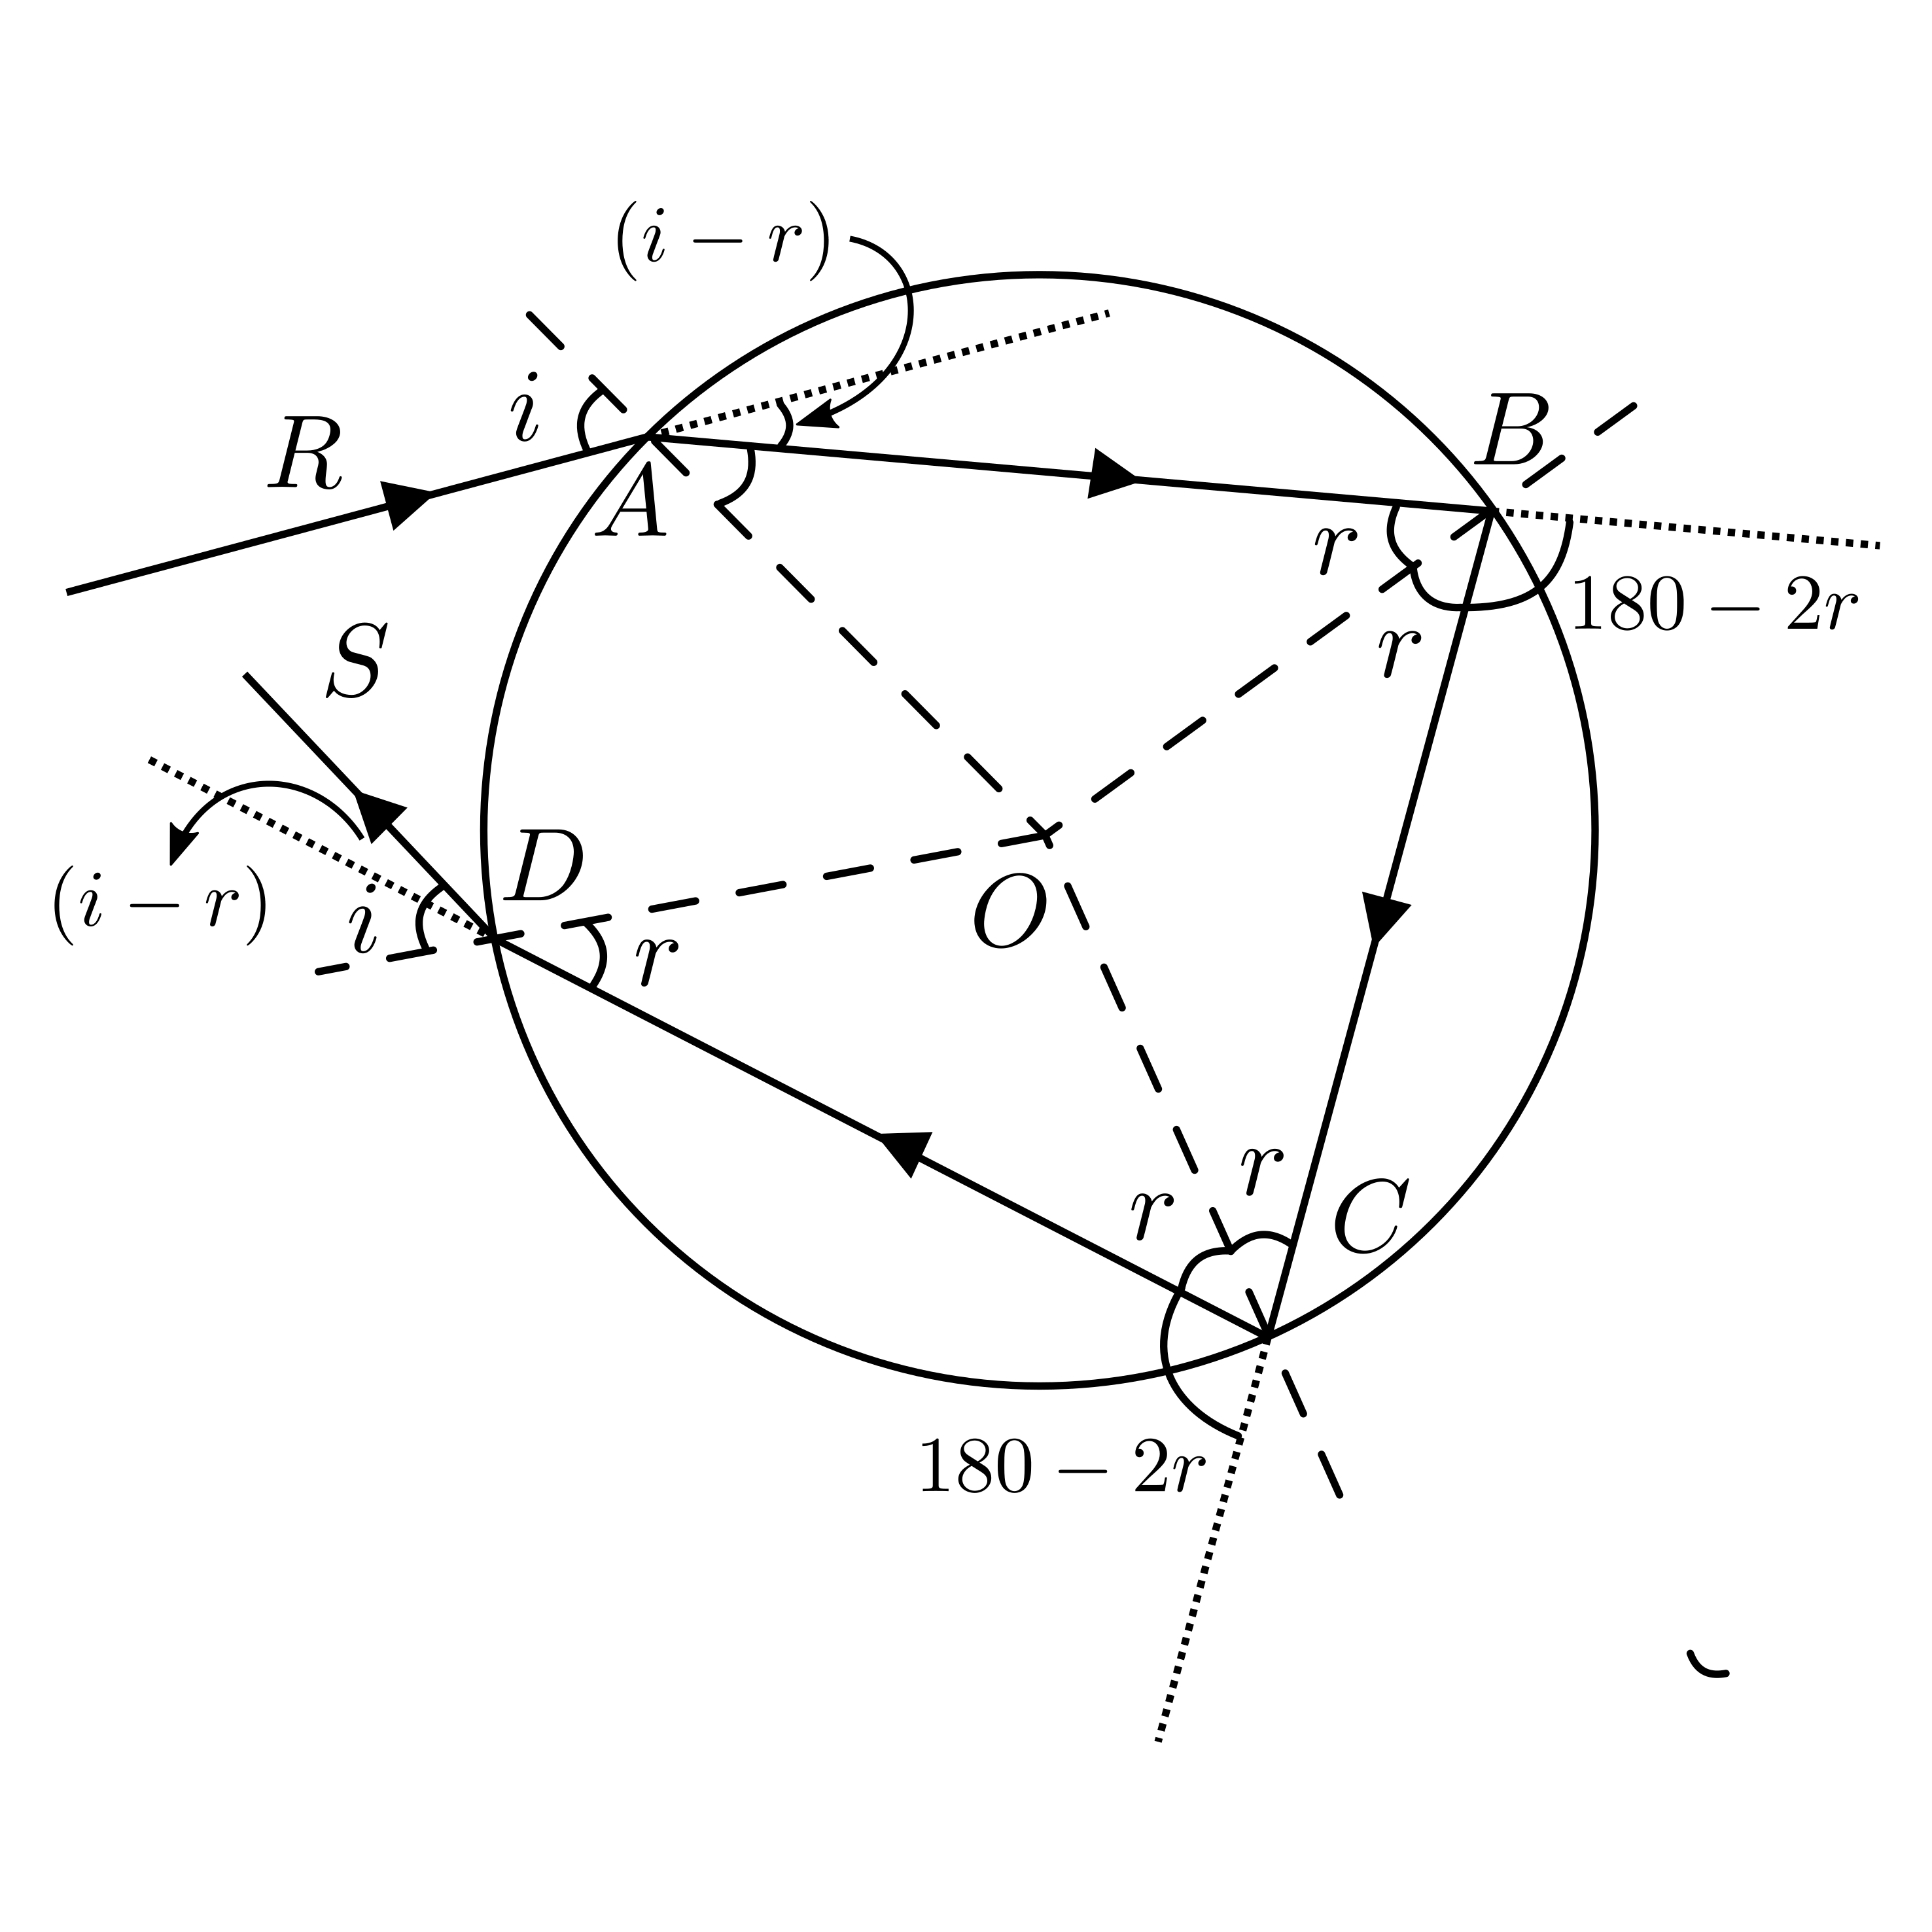
\includegraphics[width=0.5\textwidth]{figs/rainbow2.png}
    \caption{Ray diagram for the formation of a second-order rainbow, with angles marked.}
    \label{fig:secondOrder}
\end{figure}



We can now generalise this: for a $K^\text{th}$ order rainbow (corresponding to $K$ internal reflections), the deviation is $K\times(180 - 2r)$. As there are only two refractions (one at the point of incidence, and one at the point of emergence), the total deviation $\phi_K$ suffered by the emergent ray after $K$ internal reflections will be

\begin{equation*}
    \phi_K = 2(i-r) + K(180-2r),
\end{equation*}

or more simply, 

\begin{equation}
    \phi_K = 180K + 2i - 2r(K+1)
    \label{mindevK}
\end{equation}


\subsubsection*{The angle of minimum deviation}

Let us go back to look at the first order rainbow. We have:

\begin{equation*}
    \phi_1 = 180 + 2 i - 4 r
\end{equation*}

\begin{question}
\paragraph{Question:} Show that the angle $\varphi$ between the initial and and final ray is given by 
\begin{equation}
    \varphi = 4 r - 2 i
\end{equation}
\end{question}


Using Equation (\ref{snell}), we can express $r$ in terms of $i$ and $\mu$. For a drop of refractive index $\mu$, we can rewrite it as:\footnote{The refractive index of air can be taken to be $1$.}

\begin{equation}
    \mu = \frac{\sin{i}}{\sin{r}}
    \label{snellir}
\end{equation}

 or equivalently,
 
 \begin{equation}
     r = \sin^{-1}\left(\frac{\sin{i}}{\mu}\right).
     \label{rasfnofu}
 \end{equation}

The calculation of $\varphi$ shows that it increases from zero at $i=0$, to a maximum value of $42^\circ$, and then drops to about $14^\circ$ at $i=90^\circ$. Consequently, the angle $\phi_1$ \textit{decreases} from $180^\circ$ to a minimum value of $137.6^\circ$ (as can be seen in Figure (\ref{fig:minDevGraph})). At this angle, the emergent ray is deviated the \textit{least} from the direction of the incoming sunlight.

\begin{figure}[!htb]
    \centering
    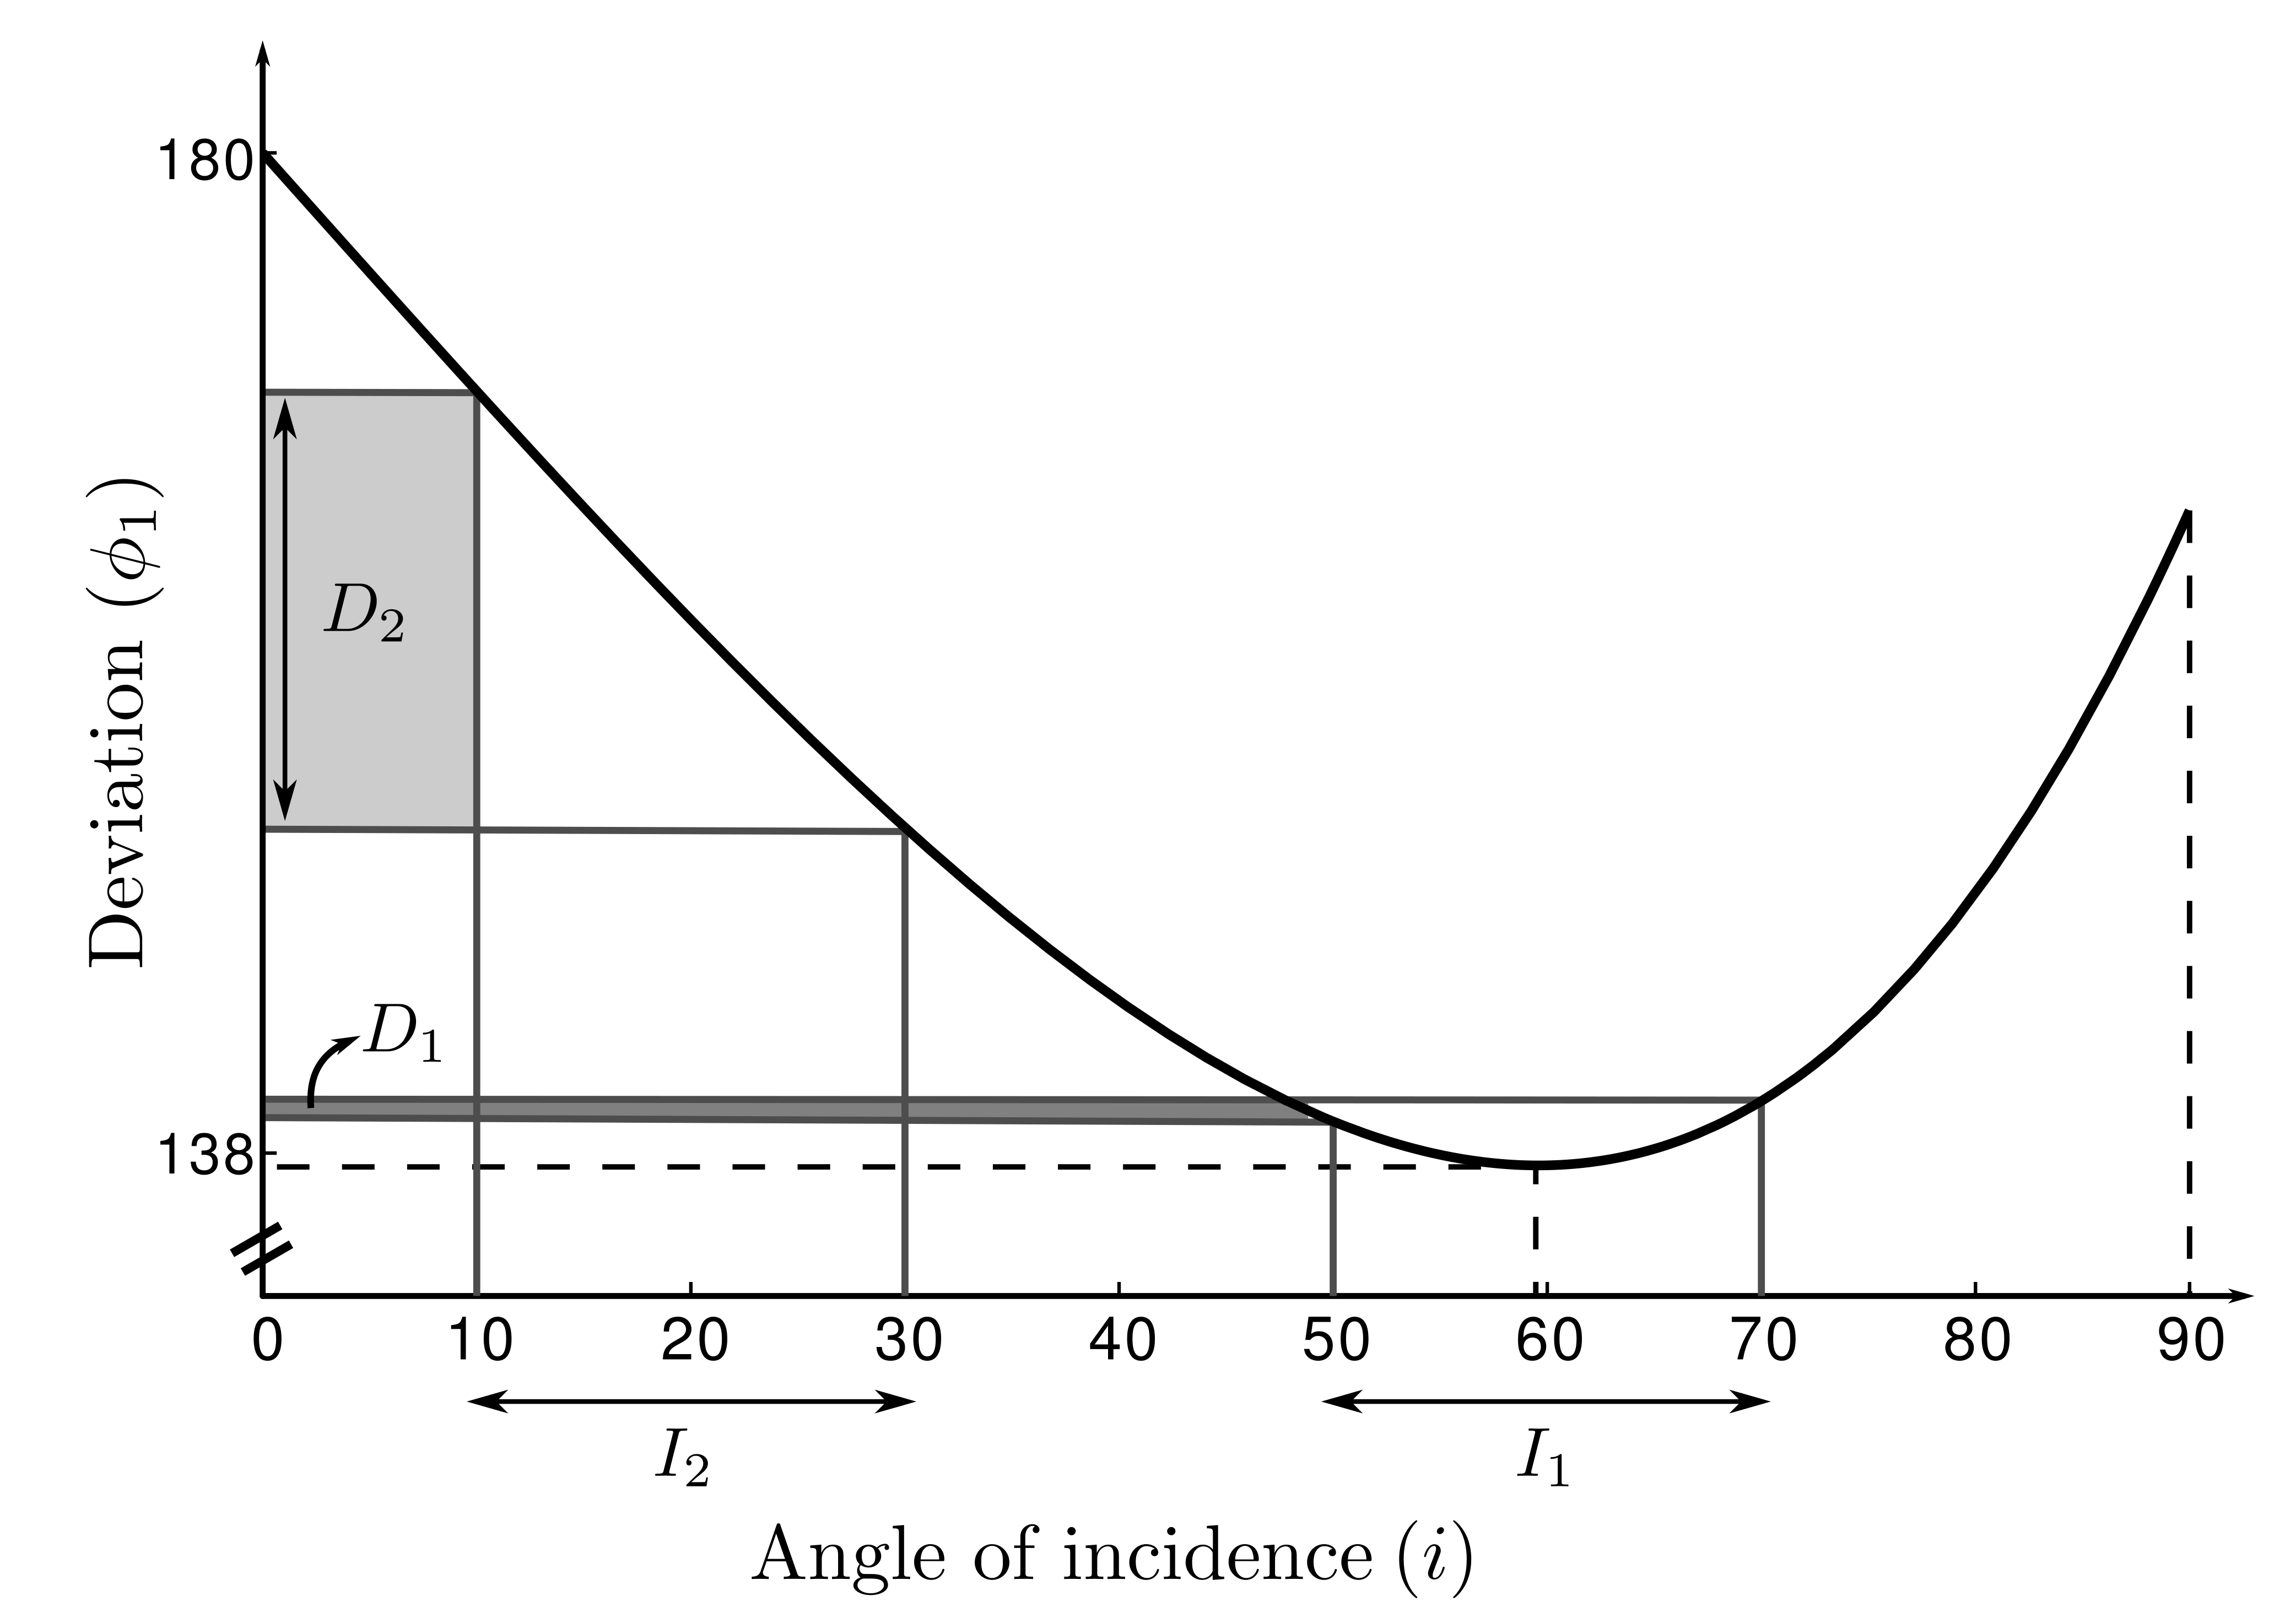
\includegraphics[scale=0.5]{figs/minimumDevGraph.png}
    \caption{The angle of deviation approaches a minimum value of around $138^\circ$ at $i=59.4^\circ$ ($r=40.2^\circ$ and $\varphi_1^\text{max} = 42^\circ$). The significance of this minimum is that rays from a range $I_1$ around the minimum ``bunch'' closer together than those from a range $I_2$ centred around some other point.}
    \label{fig:minDevGraph}
\end{figure}

However, for us to actually \textit{see} the rainbow, the different rays would nee to be ``bunched'' together, producing a higher concentration of rays that can be detected by our eyes. This is the significance of the angle of deviation being minimum: as shown in Figure (\ref{fig:minDevGraph}), consider an interval $I_1$ centred on the minimum and an interval $I_2$ of the same width centred elsewhere. The range of deviation angles for values in $I_1$ (given by the interval $D_1$) is much smaller than the range of deviation angles for values in $I_2$ (given by the interval $D_2$). Thus, rays that hit the droplet with angles $i$ in $I_1$ stick closer together than rays in $I_2$.

The reason that the rainbow appears coloured is that water has a slightly different index of refraction at different wavelengths causing this angle of minimum deviation -- known as the ``rainbow'' angle -- to vary with wavelength. In water droplets the angle of minimum deviation is $137.6^\circ$ for red light and $139.4^\circ$ for blue light. The arc of the rainbow comes from the fact that in order to see a rainbow, we must look at any direction which is at an angle of roughly $138^\circ$ from the sun's direction,\footnote{Or $42^\circ$ from the antisolar point.}, and this condition describes a circle as shown in Figure (\ref{fig:rainbowSky}). Thus, the rainbow is formed at a particular angle in the sky, and this angle is a function of the refractive index of the droplet.


\begin{figure}[!htb]
    \centering
    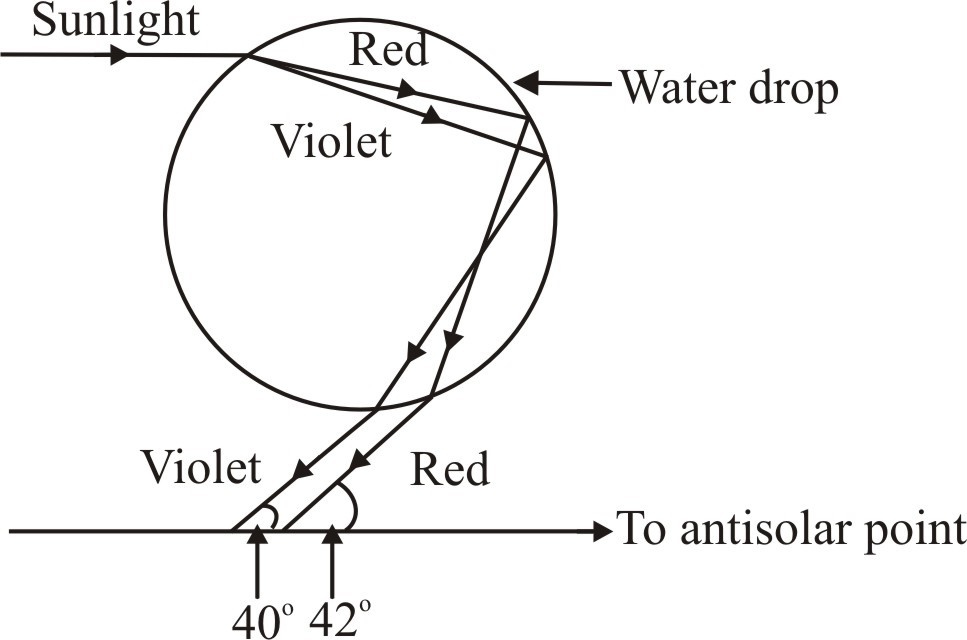
\includegraphics[width=0.5\textwidth]{figs/img1.jpg}
    \caption{Ray diagram showing the dispersion of light within the droplet. The rainbow is thus seen roughly between $40^\circ$ and $42^\circ$ from the anti-solar point.}
    \label{fig:dispersionInDrop}
\end{figure}


\begin{figure}[!htb ]
    \centering
    \includegraphics[scale=0.75]{figs/rainbowAtBeach.png}
    \caption{The rainbow in freshwater raindrops is extended below the horizon by a rainbow in seawater spray. The refractive index of saltwater drops causes the radius of the sub-horizon rainbow to be $0.8^\circ$ less than that of the above-horizon freshwater rainbow. Solar elevation is $32.5^\circ$. \texttt{Photograph taken by J. Dijkema in the Pacific Ocean, 800 km southeast of Japan, during 1981. © G.P. Können. Source:~\cite{konnen_rainbows_2017}}}
    \label{fig:rainbowAtBeach}
\end{figure}

% The rays that make up the rainbow were reflected at least once inside the drop, but not all the reflected rays contribute; the rest emerge at different angles and are not visible to the observer. The main reason higher-order rainbows are not visible in the sky is the glare of sunlight directly transmitted or reflected from raindrops. In our experiment too this `glare' tends to obscure the rainbows, but it is more easily controlled. Since only the light falling on a part of the drop contributes to a given rainbow, and the bright glare spots often result from light striking another part, it is therefore possible reduce the glare by masking a part of the incident beam.

% Let us thus imagine that only half the drop is illuminated (as will be done in this experiment): all the parallel rays are refracted when they enter the drop, and then reflected by the interior surface before being refracted as they leave. It should be clear (as can be seen in Figure (\ref{fig:rainbowDeviation})) that the emerging light is scattered over a large range of angles, depending on where the deviating ray makes contact with the drop's surface. At a certain position in the drop, a \textbf{minimum deviation point} is reached. Rays that strike the drop around this point are `bunched' together, and their brightness is further enhanced. It is precisely this phenomenon that makes the rainbow more visible in the sky than other scattered light. 


\begin{figure}[!htb]
    \centering
    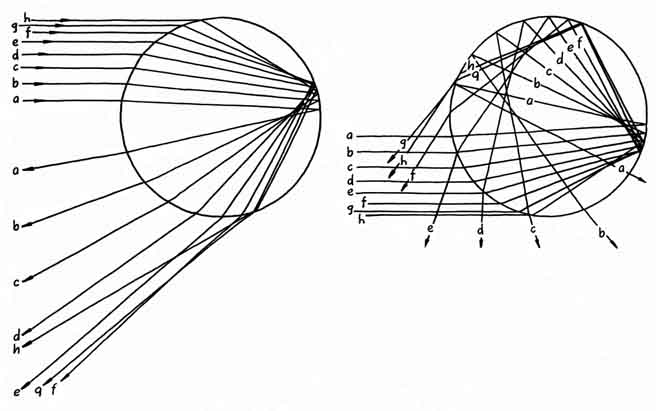
\includegraphics[width=0.75\textwidth]{figs/rainbowDeviation.jpeg}
    \caption{Ray paths forming a primary rainbow (\textit{left}) and a secondary rainbow (\textit{right}): The rays $f$ and $g$ in the primary rainbow and $g$ and $h$ in the secondary rainbow are `bunched' together as they are close to the angle of minimum deviation. \texttt{Source:~\cite{walker_multiple_1976}}}
    \label{fig:rainbowDeviation}
\end{figure}



We will thus observe the rainbow at the minimum value of $\phi_K$ from the sun,\footnote{Or $\varphi_K = 180 - \phi_K$ from the anti-solar point: in other words, the $K^\text{th}$ rainbow will appear at an angle $\varphi_K$ from the line joining the tip of your head to the tip of your shadow's head.} which we can find by enforcing the condition\footnote{That this condition represents the case of minimum deviation is clear from the fact that if $\frac{\dd^2 \phi_K}{\dd i^2}$ is calculated, it is found to be positive.}  $$\frac{\dd\phi_K}{\dd i}=0.$$

% \begin{imp}
% The index of refraction -- which determines how much the rays are being bent on entering or leaving the drop -- is different for each colour,\footnote{You will understand why this is the case in a later course on optics.} and as a result, each colour has a different angle of minimum deviation, where the scattered light is most intense. The first-order rainbow can thus be found between 137.6 degrees (for red) and 139.4 degrees (for blue).
% \end{imp}

\begin{figure}[!htb]
    \centering
    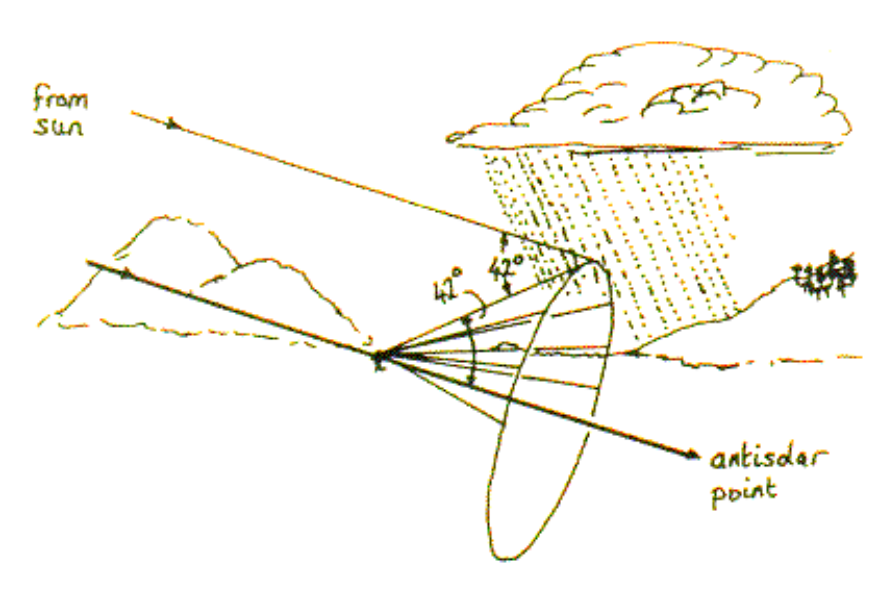
\includegraphics[width=0.5\textwidth]{figs/rainarc.png}
    \caption{Angular position of the primary rainbow in the sky.}
    \label{fig:rainbowSky}
\end{figure}


\begin{question}
\paragraph{Question:} Suppose for a moment that the refractive index of materials \textbf{didn't} depend on the wavelength of light. In this case, rainbows would:
\begin{enumerate}
\itemsep0em
    \item Remain unchanged.
    \item Not be formed.
    \item Simply be a bright white band of light.
\end{enumerate}

\paragraph{Question:} In Figure (\ref{fig:rainbowAtBeach}), is the refractive index of salt water more than or less than that of the raindrops?
\end{question}

Differentiating Equation (\ref{mindevK}), we have

\begin{equation*}
\begin{aligned}
\frac{\dd\phi_{K}}{\dd i}&=2-2\frac{\dd r}{\dd i}-2K\frac{\dd r}{\dd i}\\
&=2-2(K+1)\frac{\dd r}{\dd i}\\
\frac{\dd \phi_{K}}{\dd i}&=0\Rightarrow2-2(K+1)\frac{\dd r}{\dd i}=0
\end{aligned}
\end{equation*}

Hence,         
\begin{equation}
    \frac{\dd r}{\dd i}=\frac{1}{K+1}
    \label{mindevcond}
\end{equation}

Thus, for a $K^\text{th}$ order rainbow at the angle of minimum deviation, Equation (\ref{mindevcond}) relates the angle of refraction to the angle of incidence. 

We can use  Equations (\ref{rasfnofu}) and (\ref{mindevK}) to relate the total deviation $\phi_K$ for the $K^\text{th}$ order rainbow to the angle of incidence $i$ and the refractive index $\mu$:
 
 \begin{equation}
     \phi_K = 180K + 2i - 2(K+1)\sin^{-1}\left(\frac{\sin i}{\mu}\right)
     \label{phiKi}
 \end{equation}

In particular, for $K = 2$, one can show -- using Equations (\ref{phiKi}) and (\ref{iK}) -- that 

\begin{equation}
   \cos\left( \frac{\phi_2}{6}\right) = \frac{1}{\mu}\left( 3 \cos\left(\frac{i + 180}{3}\right) \cos{i} + \sin\left(\frac{i + 180}{3}\right)\sin{i} \right)
\end{equation}


We could also derive a relation between the angle of incidence and the refractive index for different orders of rainbows. Differentiating Equation (\ref{snellir}) with respect to $i$, we obtain,
 \begin{equation*}
     \cos i = \mu\cos r \frac{\dd r}{\dd i}
\end{equation*}

Substituting the expression for $\frac{\dd r}{\dd i}$ from Equation (\ref{mindevcond}) in the above equation, and using the Snell's law relation and the trigonometric identity, $\sin^2 x + \cos^2 x = 1$, we have
\begin{equation}
\cos i=\frac{\sqrt{\mu^{2}-\sin^{2}i}}{K+1}
\end{equation}
Squaring both sides, and using the same trigonometric identity again, the equation $(K^2 + 2K)\cos^2 i = (\mu^2 - 1)$ is obtained.
Hence, we have
\begin{equation}
    \cos i = \sqrt{\frac{\mu^2 - 1}{K(K+2)}}.
    \label{iK}
\end{equation}
 
 
\begin{figure}[!htb]
    \centering
    \begin{subfigure}[b]{0.5\linewidth}
    \centering
    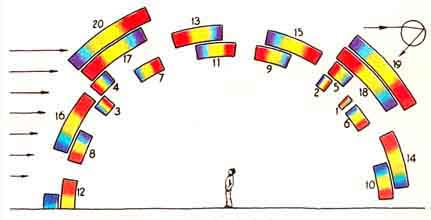
\includegraphics[width=\textwidth]{figs/multipleRainbows.jpeg}
    \end{subfigure}%
    \begin{subfigure}[b]{0.5\linewidth}
    \centering
    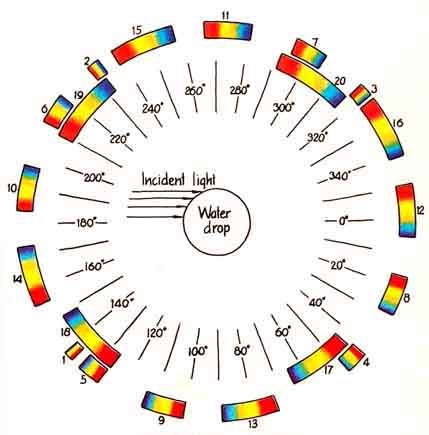
\includegraphics[width=0.75\textwidth]{figs/multipleRainbowsLab.jpeg}
    \end{subfigure}
    \caption{Rainbows represented as they would appear in the sky (\textit{left}) and in this experiment (\textit{right}), relative to the incident beam of light. \texttt{Source:~\cite{walker_multiple_1976}}}
    \label{fig:rainbow}
\end{figure}

 
\section*{Experimental Setup}

\subsection*{Apparatus}

\begin{enumerate}
\item A modified spectrometer 
\item An incandescent lamp
\item A power supply for the lamp
\item A holder for the syringe 
\item Four small syringes 
\item Four small beakers 
\item Four small Petri dishes 
\item A magnifying reading torch 
\item Water, glycerine, clove oil, and an unknown liquid A (5 ml each)
\item A spirit level 
\item Light blocking screen
\end{enumerate}


\subsection*{Description}

\begin{description}
    \item[The (modified) spectrometer]

    A spectrometer is an optical instrument, which may be used to study the spectrum of light, and can in particular be used to measure angles. It consists of four parts: a collimator, a telescope, a prism table and a circular scale disc.

    The \textbf{collimator} is used to obtain a parallel beam of light. The collimator is a tube with a lens at the back (called the collimator lens) and an adjustable slit at the front. The distance between the slit and the collimator lens can be adjusted with the help of a knob fixed to its body. The \textbf{telescope} is used to collect and observe parallel light. The telescope is another tube with an arrangement of lenses (called the objective and the eyepiece) at the ends. The distance between the objective and the eyepiece may also be adjusted. The \textbf{prism table} is a circular table with levelling screws, which is mounted at the centre of the circular scale disc. The prism table is used to mount optical components (prisms, obviously, but also gratings, etc.).  The \textbf{circular scale disc} is used to measure and record the position of the telescope arm and thus measures the angle of displacement. The circular scale disc has three scales, a circular main scale and two identical vernier scales. The vernier scales are fixed along two windows to the prism table and the circular main scale moves with telescope arm.  

    \textbf{Modifications:} In the modified spectrometer, the mounting base of the collimator arm has been extended to move the collimator away from the circular base and hence increase the range of movement of the telescope. The collimator is provided with an extra adjustable slit mounted externally on its back. This extra slit allows us to block the light falling on one side of the liquid drop so that only one half of the liquid drop is illuminated. The telescope does not have the regular lens arrangement, but instead the eyepiece is replaced by a pinhole and the objective is replaced by a lens of suitable focal length. This is done to obtain a magnified image of the drop. The circular scale disc is kept as it is. 

    A specially designed holder is fixed on the prism table, within which a syringe may be clamped. The holder is designed so that when the syringe is clamped properly and the drop is obtained, the drop is seen from all the angular positions of the telescope exactly at the centre of field of view. 

    \begin{figure}[!htb]
        \centering
        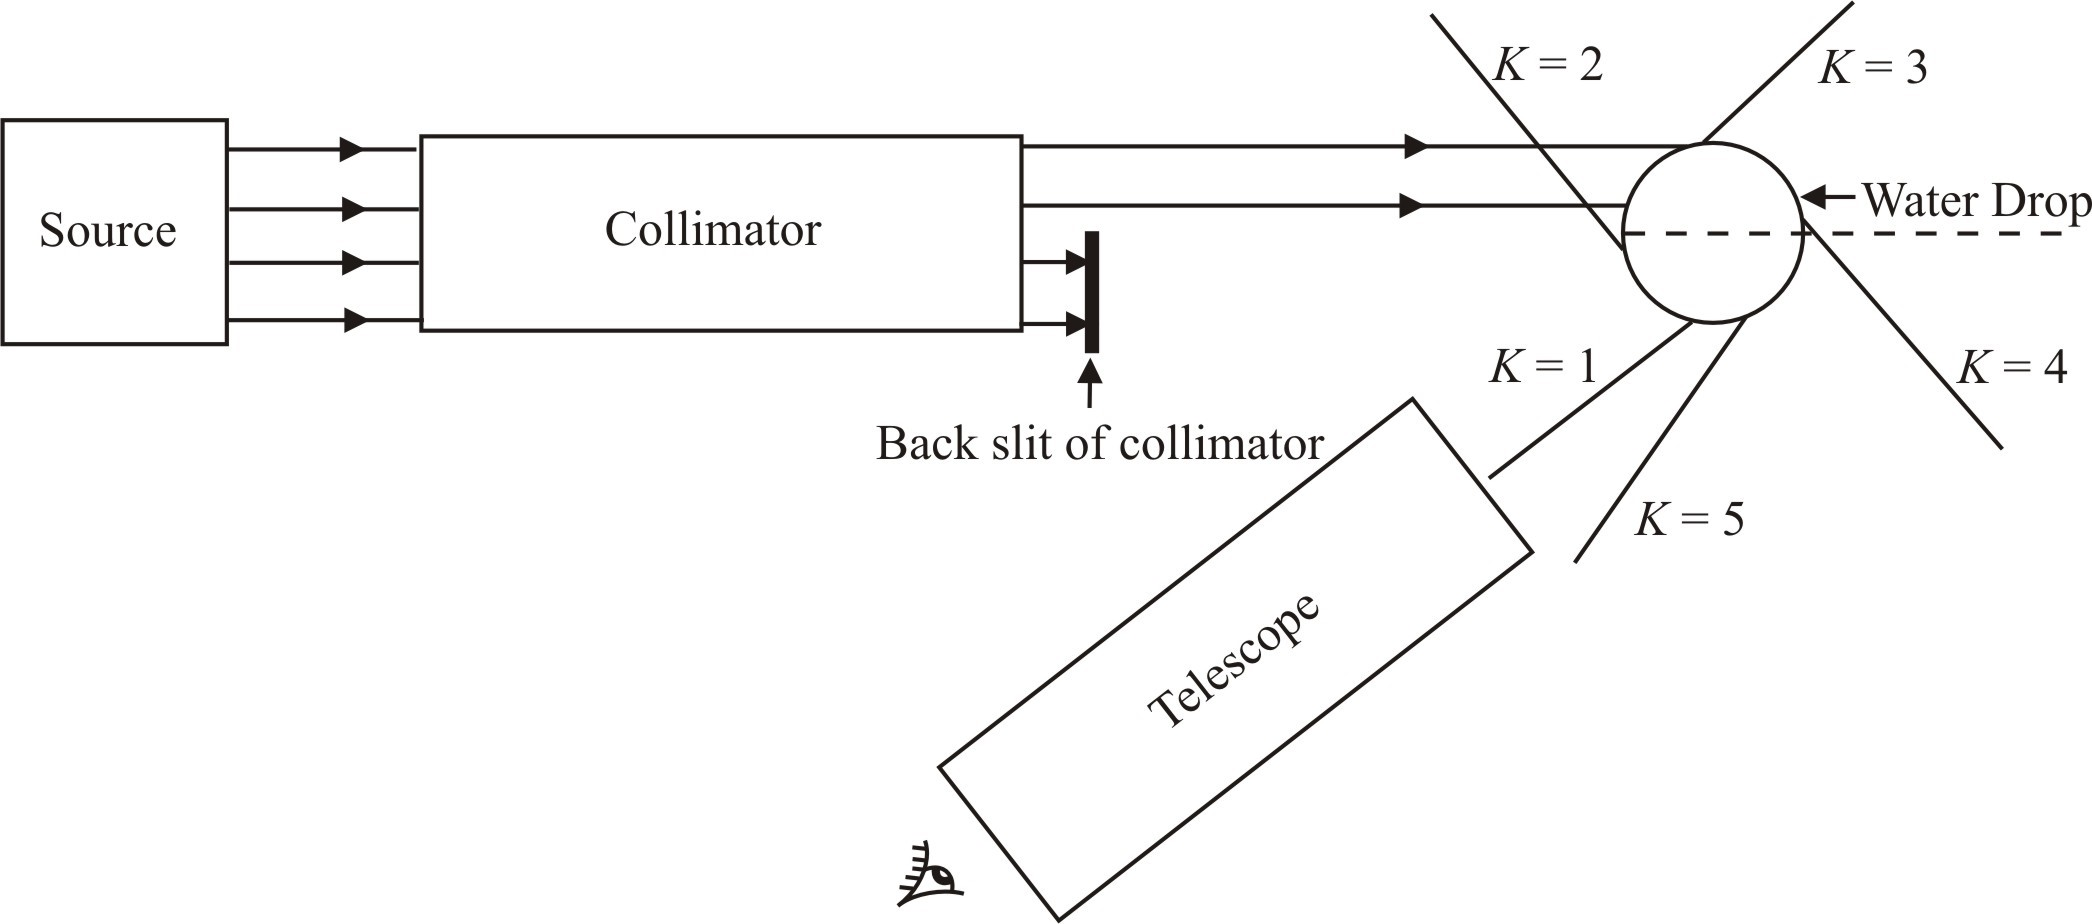
\includegraphics[width=0.70\textwidth]{figs/img2.jpg}
        \caption{Schematic of the experimental setup}
        \label{fig:experimentalsetup}
    \end{figure}

    \item[Halogen lamp]

    A high power (150 W, 24 V) tungsten filament halogen lamp (such as those commonly used in projectors) is provided as a source of white light. This lamp has a small filament, through which a high current (6 A) can be passed. It is mounted in a wooden box, on a stand whose height may be adjusted. The wooden box has four windows through which the light may be observed. A small fan is fixed inside the box to prevent excessive heating. The lamp has a specially designed 24 V (AC) power supply which powers it. The intensity of light emitted by the lamp may be changed on the supply. This is essential for observing the higher-order rainbows, as one may need to have white light of higher intensity.

    \item[Miscellaneous]
    A set of four small syringes, beakers, and Petri dishes are provided. Beakers may be used to store different liquids. Petri dishes can be placed on the prism table and are used to collect the liquid that falls from the syringe. Four different liquids (water, glycerine, clove oil, and an unknown liquid A) are also supplied. A magnifying reading torch is provided to read the circular scale, and a light blocking screen may be used to block the stray light falling on the drop. A spirit level may be used for levelling the prism table.

\end{description}


\subsection*{Useful Data}
\begin{itemize}
    \item Refractive index of water = 1.33
    \item Refractive index of glycerine = 1.47
    \item Refractive index of clove oil = 1.53
\end{itemize}

\subsection*{Precautions}
\begin{itemize}
\item Avoid observing the source directly through the telescope for long time.
\item Clamp the syringe on its holder carefully, so that it is held properly.
\item Use different Petri dishes, beakers, and syringes, for different liquids to avoid mixing.
\item Light reflected directly from the external surface of the drop will produce bright white glare spots that will hinder your observations. You will have to account for this and identify the rainbows carefully. 
\item The measurements have to be performed in a dark room.
\item Use only one window of the spectrometer for recording the readings. Use the same one throughout your experiment.
\end{itemize}


\section*{Experimental Problem}
\subsection*{Part A}

In this part, you will study the formation of rainbows of different orders by a suspended drop of water and measure their angular positions. You can observe these rainbows directly with your eye and can measure their angular positions using a telescope and a circular scale. 

\begin{imp}
Begin by determining the least count of the spectrometer.
\end{imp}

\begin{enumerate}
    \item Level the prism table using a spirit level. 
    
    \item Fill the syringe with water and mount it on the holder clamped to the prism table.
    
    \item Keep the Petri dish on the prism table to collect the water drops, which may fall down from the nozzle of the syringe. 
    
    \item Obtain a steady drop of water at the nozzle of the syringe. 
    
    \item Adjust the height of the syringe such that the drop is seen at the centre of the field of view of the telescope.
    
    \begin{question}
    \paragraph{Question:} The rays of light falling on the drop \textbf{must} be parallel. How would you make sure this is the case?
    \end{question}
    
    \item Adjust the alignment of the source, the collimator, the suspended drop, and the telescope, such that the drop is fully illuminated by the parallel beam of light. Close the back slit of the collimator partially, so that only the vertical half of the drop is illuminated by white light.

    \begin{question}
    \paragraph{Question:} If the rays of light falling on the drop are parallel, does this mean that all the rays striking the drop will be refracted by the same angle? Explain your answer.
    \end{question}
    
    \item Keep the telescope, collimator, and the drop in the straight line; you will see white light coming from the central region of the drop. Note the angular position of the telescope at which this happens and treat it as the ``direct'' -- or undeviated --  reading for further measurements. As stated earlier, this drop will produce rainbows of different orders, which can be observed at different angular positions around the drop. Thus the angular positions of different order rainbows (for water) will be as shown earlier in Figure (\ref{fig:firstOrder}). 

    \item Observe the bright first-order rainbow to the right of the drop $(K = 1)$ first by eye and then by telescope. Adjust the telescope such that the bright red line of the spectrum can be seen. Measure the total angle of deviation $\phi_1$. 
    
    \item Repeat the above step for the second-order rainbow $(K = 2)$ and then for orders up to at least the fifth $(K = 5)$. (In this case you may change the intensity of lamp.) Measure the total angle of deviation $\phi_K$ for each order. (Note: Before taking readings for each order, adjust the telescope to see the red line of the spectrum.) 
    
    \item Plot a graph of $\phi_K$ against $K$ for the different order rainbows $(K = 1, 2, 3, \hdots)$ formed due to a water drop.
\end{enumerate}


\subsection*{Part B}

In this part, you will obtain the rainbows with different liquids and relate the deviation for the second-order rainbow with the refractive index of the liquids.

\begin{enumerate}
    \item Replace the syringe and Petri dish containing water by the syringe and Petri dish containing glycerine and adjust the syringe to see the glycerine drop from all the positions of the telescope.
    
    \item Measure $\phi_2$ for glycerine, following the same procedure as in \textbf{Part A}.
    
    \item Repeat the above steps, for the clove oil and the given unknown liquid $A$. Determine $\phi_2$ for clove oil and the liquid $A$.
    
    \item Plot a graph of $\cos(\phi_2 / 6)$ against $1/\mu$ for water, glycerine and clove oil. 
    
    \begin{question}
    \paragraph{Question:} When $\mu = 1$ (air), what is the value of $\phi_2$? This should be taken as one of the points for plotting the above graph.
    \end{question}

\end{enumerate}

  
 

\subsection*{Part C (\textit{optional})}


In this part, you will use the data from \textbf{Part B} to determine the refractive index of the unknown liquid $A$. 

\begin{enumerate}
    \item Measure the angle $\phi_2$ for the unknown liquid $A$, following a procedure similar to \textbf{Part A}.
    
    \item Use this value of $\phi_2$, along with the graph from \textbf{Part B}, to determine the refractive index of the liquid $A$.
\end{enumerate}



\section*{References}
% \begin{enumerate}
% \item Jearl D. Walker, \textit{Multiple rainbows from single drops of water and other liquids}, Am. J. Phys, 44 (5), 1976, pp. 421-433.
% \item Können, G.P., 2017: \textit{Rainbows, Halos, Coronas and Glories: Beautiful sources of information}, Bull. Amer. Meteor. Soc., 98, 2017, pp. 485–494.
% \item Kenneth Sassen, \textit{Angular scattering and rainbow formation in pendant drops}, J. Opt. Soc. Am., 69 (8), 1979, pp. 1083-1098. 
% \item John Beynon, \textit{Introductory University Optics}, Prentice-Hall of India Pvt. Ltd., New Delhi, 1998, pp. 44-55.
% \item Francis W. Sears, \textit{Optics}, Asian Publishing House (India), 1958, pp. 54-55. 

% \end{enumerate}

\nocite{khaparde_training_2008}
\nocite{walker_multiple_1976}
\nocite{konnen_rainbows_2017}
\nocite{sassen_angular_nodate}

\printbibliography[heading=none]

\newpage

\end{refsection}
\chapter{The Carey Foster Bridge}

\section*{Objectives}

\begin{enumerate}
\item To understand how a Carey Foster bridge works.
\item To find the value of an unknown low resistance using the Carey Foster bridge.
\end{enumerate}

\section*{Apparatus}

\begin{enumerate}[label=\arabic*)]
\itemsep0em
\item A low voltage DC power supply
\item A Carey Foster bridge
\item Two fixed standard resistances (1 or 2 $\Omega$)
\item A fractional resistance box
\item A one-way key
\item A thick copper strip
\item An unknown low resistance ($S$)
\item A null detector (galvanometer)
\item Connecting wires.
\end{enumerate}

\section*{Introduction}
\subsection*{Measurement of low resistance} 
Ohm's law, $V=IR$, states that the current flowing through a resistor with resistance $R$ varies linearly with the potential difference across it.
To measure the resistance, one method involves studying the IV characteristics of a resistor, i.e looking at the variation in the current, $I$, flowing through the resistor for a range of applied potential differences, $V$ and then extracting the value of the resistance, $R$, from the resulting graph/data. This direct application of Ohm's law usually works well for resistances in the range $1-100 \Omega$. 

\begin{figure}[!htb]
    \centering
    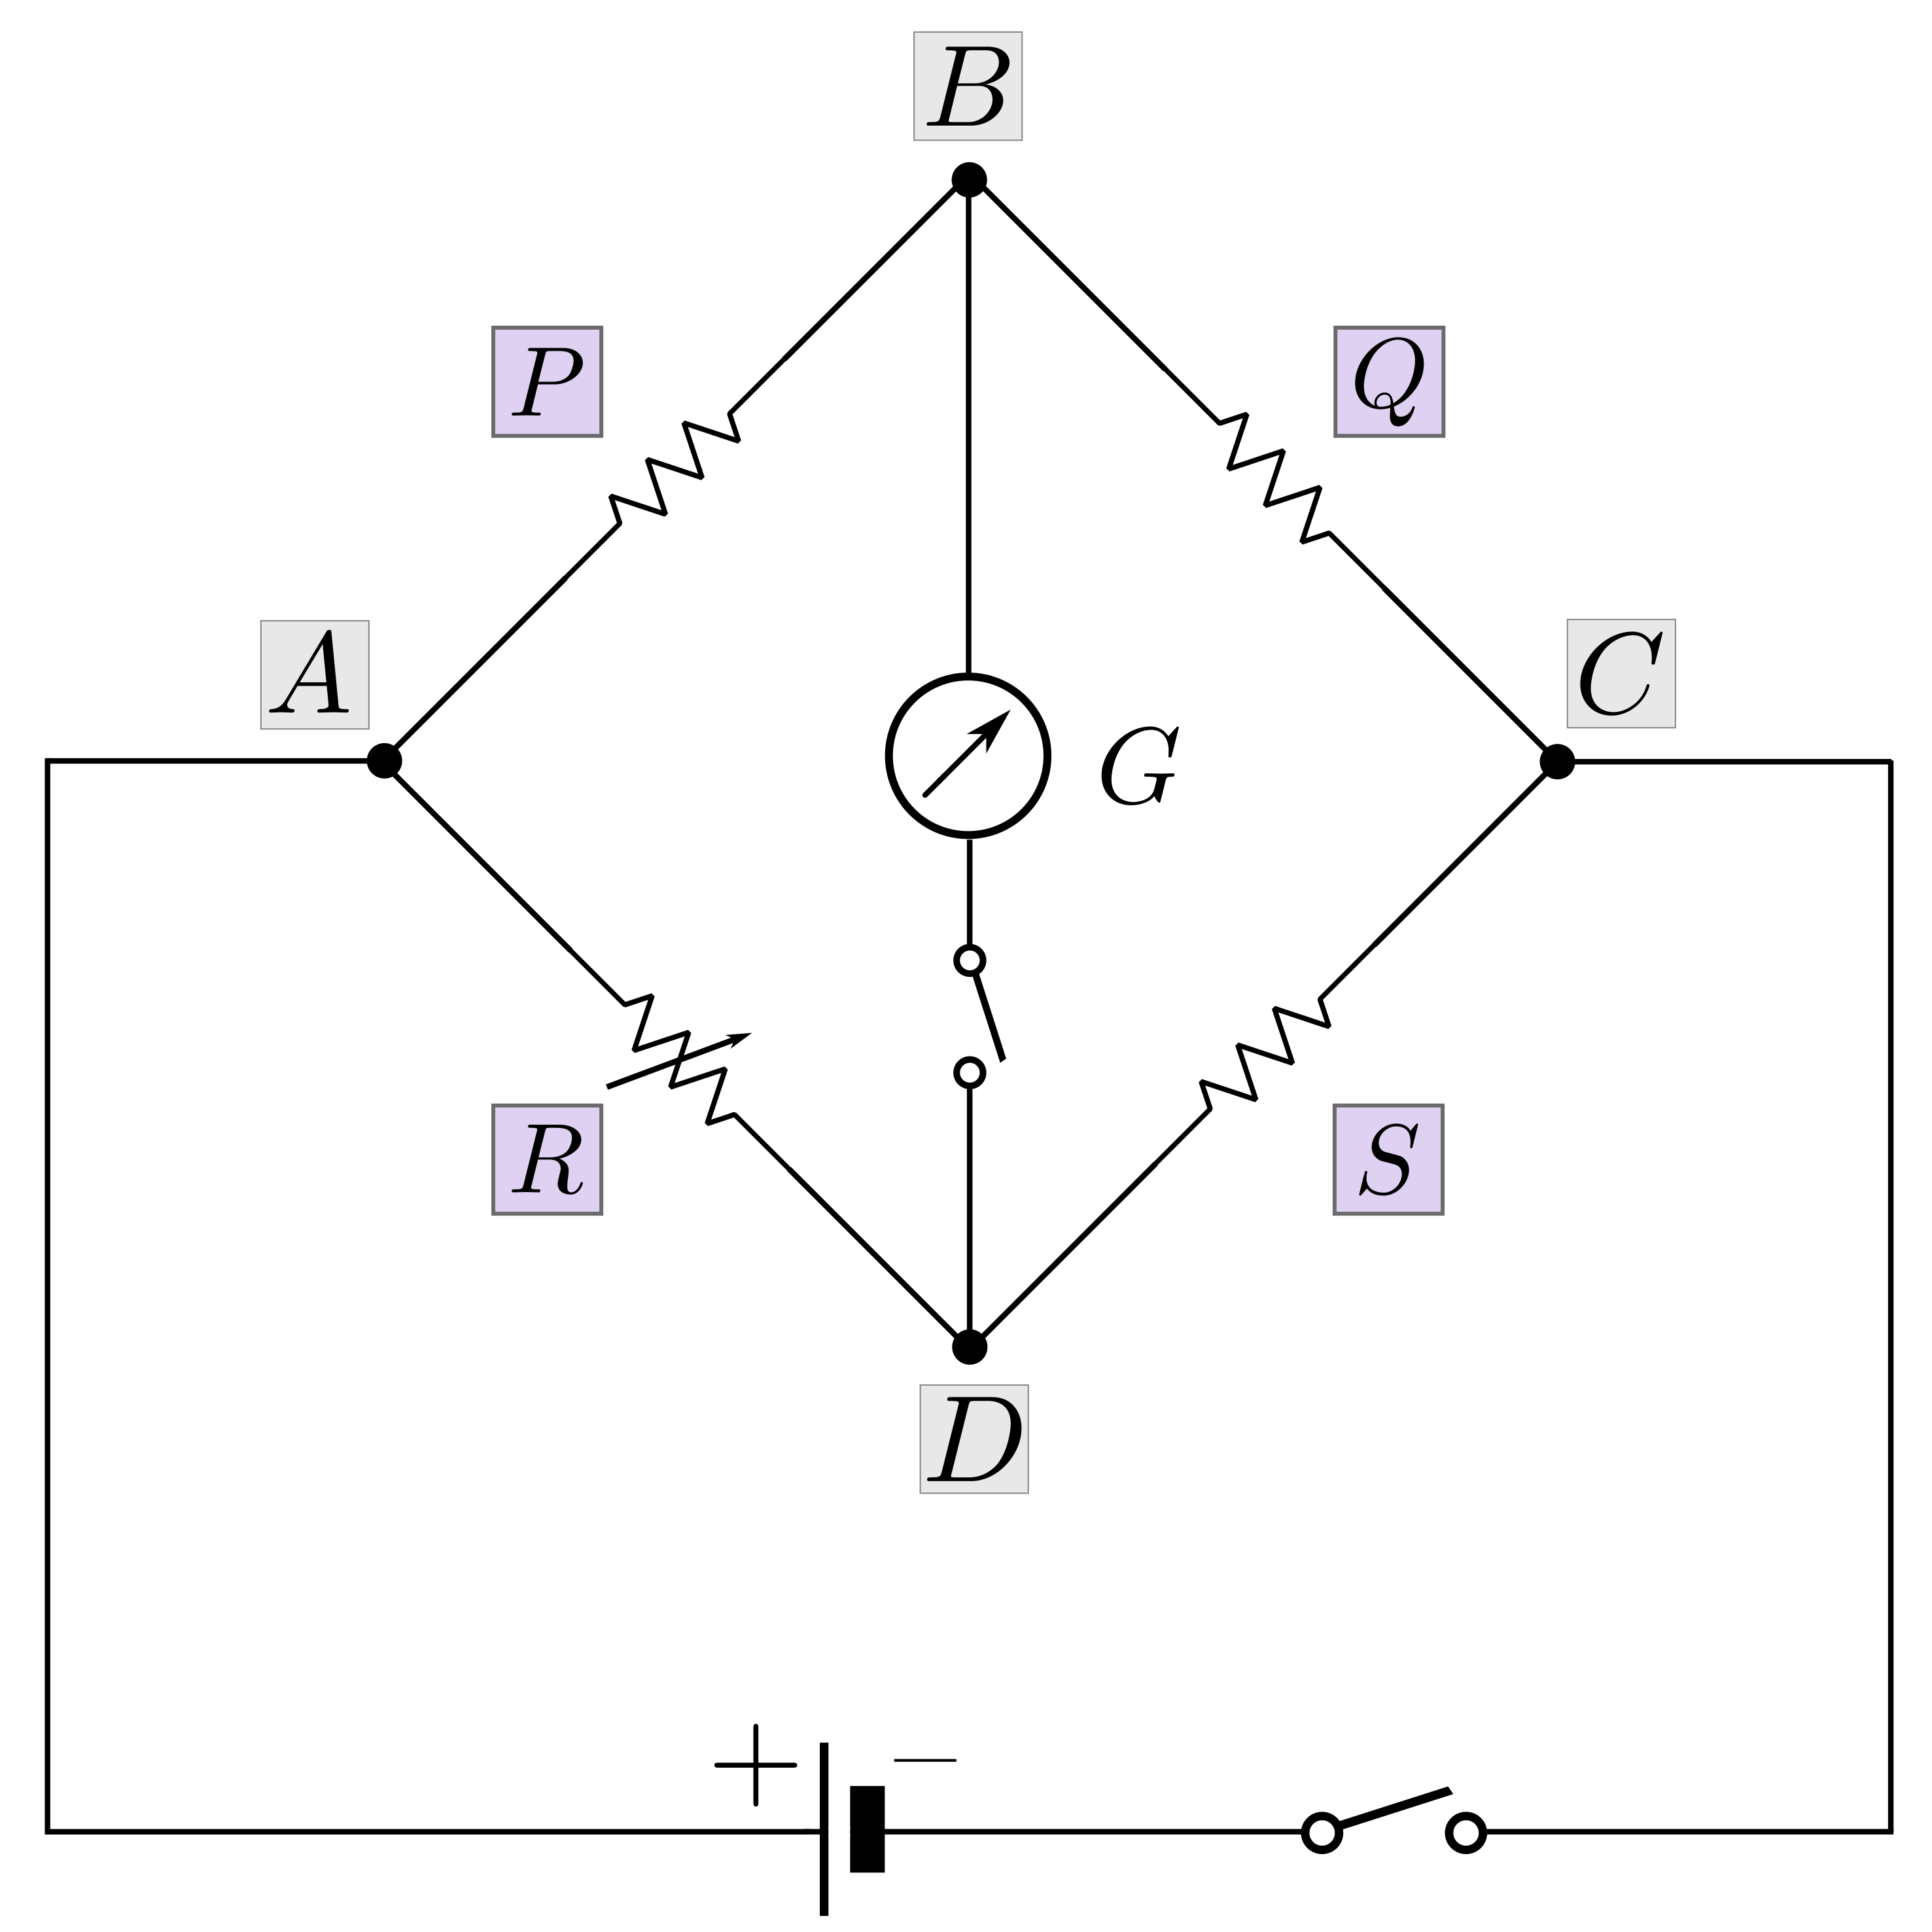
\includegraphics[width=0.5\textwidth]{figs/wheatstone.png}
    \caption{Schematic diagram of a Wheatstone bridge.}
    \label{fig:wheatstone}
\end{figure}

For the measurement of low resistances, it is preferable to use methods that work on comparison of resistances (so you would need, in the first place, some precisely known, standard resistances). Such methods are based on the principle of a Wheatstone's bridge. A Wheatstone bridge is shown in Figure (\ref{fig:wheatstone})\\
A current measuring device, the galvanometer, registers current flowing in the arm $BD$. However, when the nodes $B$ and $D$ are at the same potential, no current flows in the arm $BD$. This happens when the following relation between the resistances is satisfied
\begin{equation}
    \frac{P}{Q}  =\frac{R}{S}
    \label{balanceofthebridges}
\end{equation}
In such a situation, the Wheatstone bridge is said to be \textit{balanced}.
To find out the resistance of an unknown resistor, two standard resistors are wired in arms $AB$ and $BC$. The value of the (variable) resistor, $R$, is varied until the point of zero/null deflection/display is found on the galvanometer. Since, the bridge is now balanced, Equation (\ref{balanceofthebridges}) holds good, and we can infer the value of an unknown resistance, $S$. 
We note here that this null method, which hinges on balancing the Wheatstone bridge, is useful because by not measuring a finite value of the current, the galvanometer does not have any role to play in the accuracy of the resistance measurement, our measurement of an unknown low resistances is limited only by the precision of other resistors in the experimental setup.
In this experiment, we will use a form of modified Wheatstone bridge called a Carey Foster bridge, which is useful to measure low resistances while eliminating end corrections.

\section*{Description}

In \textbf{Part A}, you will determine the apparent value of a small resistance. 

In \textbf{Part B}, you will determine a small correction. 

%In \textbf{Part C}, 

\section*{Theory}

\begin{figure}[!htb]
    \centering
    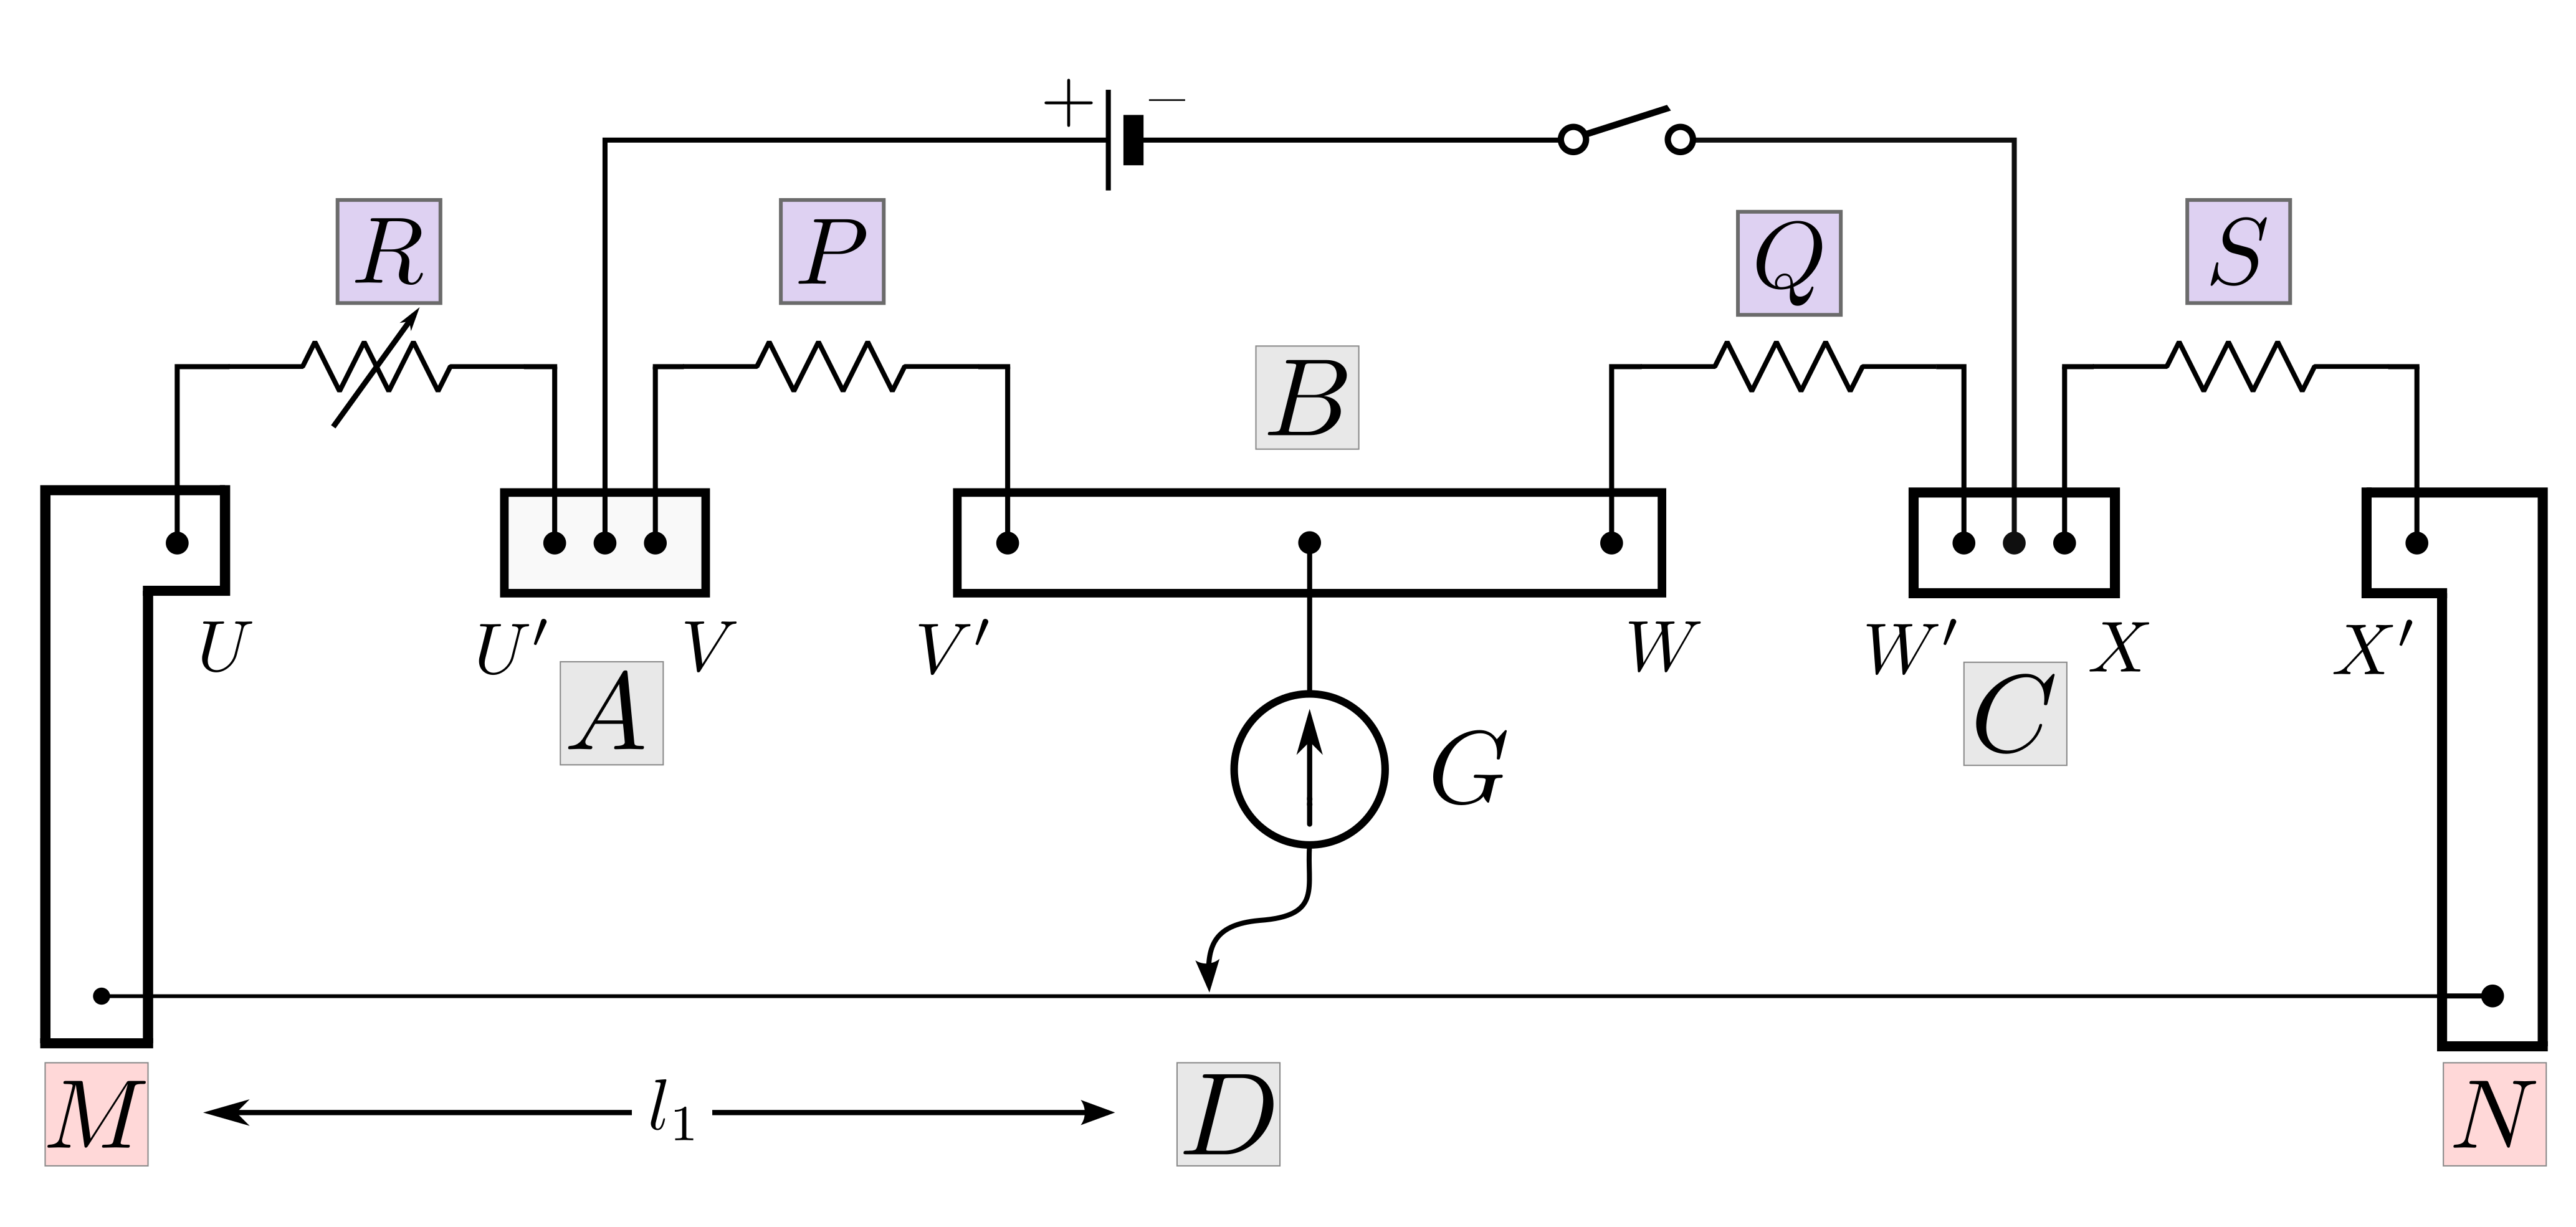
\includegraphics[width=\textwidth]{figs/carey.png}
    \caption{Schematic diagram of the Carey Foster bridge.}
    \label{fig:carey}
\end{figure}

The Carey Foster bridge with a circuit around it is illustrated in Figure (\ref{fig:carey}).
%The shaded part is a copper strip 
The bridge consists of a copper strip
with four gaps (these act as four arms of a Wheatstone’s bridge). Two known resistances $P$ and $Q$ (equal and small) are connected in the inner gaps, $VV^{\prime}$ and $WW^{\prime}$. A null detector (galvanometer) is attached between the terminal $B$ and the jockey at $D$.
A variable resistance box, $R$, with fractional resistances is placed in the outer gap at $UU^{\prime}$. The unknown (low) resistance, $S$, which is to be determined, is put in the 
outer gap at $XX^{\prime}$. A battery, a key, and a resistance box (if necessary) are connected between the terminals $A$ and $C$. A one metre long wire $MN$ of uniform resistance per unit length is mounted alongside a metre rod, and is soldered to the two ends of the copper strip. Since the jockey can be slid along the wire $MN$, the point $D$ can be anywhere between $M$ and $N$. It represents the position at which the null detector would register a value of 0. To locate this point, we tap the jockey over the wire. 

The wire, $MN$, is uniform and therefore, we may assume that it has a constant resistance per unit length, say, $r$ $ \Omega cm^{-1}$. When the point $D$, located at some distance, $l_1$, from the end $M$ is chosen such that the null detector displays $0$, from the condition of a balanced Wheatstone bridge, we have, for the Carey Foster bridge 
\begin{equation}
\frac{P}{Q}=\frac{R+\delta_{1}+l_{1}r}{S+\delta_{2}+(100-l_{1}r)}
\label{careyconfig1}
\end{equation}

Here, $\delta_{1}$ is the value of the resistance at the soldered junction, $M$, and $\delta_{2}$ is the value of the resistance at the junction $N$. These are the end/contact resistances. It is easy to account for these end corrections using a simple technique - we interchange the resistances, $R$, and $S$ - the unknown resistance is now connected in gap $UU^{\prime}$, while the resistor $R$ is placed in gap $XX^{\prime}$. Expectedly, the location of the null point on the wire $MN$ changes which, assume, is now located at a distance $l_2$ from the end $M$. The condition of balance is now the following
\begin{equation}
\frac{P}{Q}=\frac{S+\delta_{1}+l_{2}r}{R+\delta_{2}+(100-l_{2}r)}
\label{careyconfig2}
\end{equation}

Equations (\ref{careyconfig1}) and (\ref{careyconfig2}), together, yield the \textit{nice} (independent of end corrections) relation - 
$S = R + (l_1-l_2)r$. Clearly, from an experiment that involves measurements of $l_1$ and $l_2$ for an appropriate range of resistances, $R$, one can deduce the value of the unknown resistance, $S$ and also the resistance per unit length of the bridge wire. 
\\

\begin{question}
\paragraph{Question:} Can we exchange the position of battery and the galvanometer? Which is the preferred arrangement and why?~\\
\paragraph{Question:} Why does the procedure involve interchanging R and S?~\\
\paragraph{Question:} Draw the equivalent Wheatstone Bridge.~\\
\paragraph{Question:} How is the Carey Foster an improvement over a standard Wheatstone bridge?~\\
\paragraph{Question:} What is the largest unknown resistance that can be measured using a Carey Foster bridge?
\end{question}


\section*{Experimental Setup}

\subsection*{Warnings}
\begin{enumerate}
    \item Clean all contacts thoroughly including %the battery terminals 
    the teeth of the alligator clips with sand paper.
    \item Make sure that enough wire is exposed while making connections, so that insulation does not come in between.
    \item Check each contact by tugging on the wire and ensuring that it does not loosen or come undone. 
    \item Arrange the elements of the circuit, so that it resembles your circuit diagram.
    \item While making the circuit think in terms of loops, not in terms of terminals. 
    \item Make sure there is a finite resistance in the circuit, \textit{before} the key is closed.
    \item Measure all balance lengths from the same side and on same scale.
\end{enumerate}


\section*{Procedural Instructions}

\begin{imp}
Before starting observations, \textit{test} and \textit{debug} your circuit. Some common methods of debugging include checking the DC supply potential, checking continuity of your circuit using a multimeter. If there is no potential drop across a passive element, then check for continuity.
\end{imp}


\subsection*{Part A}

\begin{enumerate}
    \item Make the connections as shown in the circuit diagram and connect the DC source. $S$ is the unknown resistance.
    \item Take out the zero resistance key from the resistance box ($R$) and note down the balance length ($l_1$). When determining the balance point, approach it from both sides and determine the range, if any, over which you get a null deflection. 
    \item Change the resistance in the box and find the new balance length.
    \item Interchange the position of the unknown resistance and the resistance box and repeat steps 1 to 3 to determine $l_2$.
    \item Tabulate $l_1 + l_2$.
    \item Plot a graph between $R$ and $l_1 -l_2$.
    \item Use this graph to determine the the resistance per unit length of the wire, and the apparent value of the unknown resistance.
\end{enumerate}

\subsection*{Part B}

\begin{enumerate}
    \item Make the connections as shown in the circuit diagram and connect the DC source. ($S$ is a copper strip.)
    \item Take out the zero resistance plug from the resistance box ($R$) and note down the balance length ($l_1$). To make sure you are indeed at the balance point, infinitesimally moving the jockey, \textit{on either side}, should correspond to a small but finite current value on the galvanometer.
    \item Vary the resistance in the resistance box and find the new balance length.
    \item Interchange the position of the copper strip and the resistance box and repeat steps 1 to 3 to determine $l_2$.
    \item Tabulate $l_1 + l_2$.
    \item Plot a graph between $R$ and $l_1 -l_2$ on the same graph sheet as the one on which you plotted the readings in part A. 
    \item Examine the two lines carefully and check (i) whether they are parallel and (ii) what the apparent resistance of the copper strip is. 
    \item The unknown resistance in part A is not equal to the intercept but the difference between the intercepts of the lines in parts A and B. 
    
\end{enumerate}

\begin{question}
\paragraph{Question:} Why have you been asked to tabulate $l_1 + l_2$ even though it is not used in the calculations?~\\
\paragraph{Question:} Why do the two lines -- from parts A and B -- need to be parallel?~\\
\paragraph{Question:} Explain the correction factor determined in part B. 
\end{question}

\section*{References}

\begin{enumerate}
\item Advanced Practical Physics for Students, B. L. Worsnop, and H. T. Flint
\item Experiment 6, Measurement of Low Resistance using the Carey Foster Bridge, National Digital Repository (eGyanKosh)
\end{enumerate}


\newpage

% \vbox
% {\textcolor{Blue}{\part{Lecture Demonstrations}}
% \tikz[remember picture,overlay]\node[shift={(-1,1)},opacity=0.6] at (current page.south east) {
\includegraphics[width=17.5cm]{logo}};
% }

% \renewcommand{\chaptername}{Lecture}

% 
\title{Lecture Demonstration}
\author{An Introduction to Physics through Experiments}
%\date{5th April, 2018}
\date{}

\maketitle
\section{The quality of light}

\subsection{Introduction}

\vspace{0.5cm}

I have always found the study of light to be quite confusing and have only recently been able to properly appreciate why, as well as the richness that the study of light lends itself to. 

For starters, light as a classical wave forms the center of Classical Electromagnetism that you will be studying in some detail in the next semester. 


\begin{tcolorbox}
\paragraph{Question: }Consider the following properties of light:

\begin{enumerate}
\item Wavelength
\item Frequency
\item Speed
\item Energy
\item Polarisation
\end{enumerate}

Which (if any) constants of Nature are associated with them?
\end{tcolorbox}

\vspace{0.5cm}

As a fundamental particle, light is described quantum mechanically as a quantum of energy. The fact that it travels at $c$, the speed limit of the universe, is a reflection of the fact that it is a highly relativistic particle.

Throughout this class we will be jumping between different ways of looking at light, and I feel that this is something you should be comfortable doing yourself, eventually.

\subsection{Colours}

Let us begin with an analysis that is not at all rigorous. The light that you see is a combination of different wavelengths. These forms a very small part of what we call the `electromagnetic spectrum', which ranges all the way from gamma radiation and x-rays to microwaves and radiowaves. The property of colour, however, is only associated with light that falls between the convenient wavelengths of around 400 -- 800 nm, the \textit{visible spectrum}.

Objects appear different colours because they absorb certain wavelength and reflect (or transmit) others. The rods and cones in your eyes detect the intensities and wavelengths of the reflected or transmitted rays and send them to the brain for interpretation. Thus `white' and `black' are not colours in strictest of senses, as they have no specific wavelength of light associated with them. The brain associates an object with the colour white when it reflects all the wavelengths of visible light incident on it, and similarly associates an object with the colour black when it absorbs all (or reflects \textit{none}) of the wavelengths of visible light incident on it. 

For example, a red object looks red because the dye molecules in the paint on it have absorbed the wavelengths of light from the violet/blue end of the spectrum, reflecting only `red' light. If only blue light is shone onto a red shirt, the shirt would appear black, because the blue would be absorbed and there would be no red light to be reflected. When you look at an object, perceiving a `distinct' color, you are not necessarily seeing a single wavelength of light. When you look at an object that appears red to your eye, there may be several frequencies of light striking your eye with varying degrees of intensity. Your eye-brain system, however, interprets the frequencies that strike your eye, interpreting the colour as being `red'.

\begin{tcolorbox}
\paragraph{Question: } Is magenta part of the visible spectrum? If so, at approximately what wavelength is it?
\end{tcolorbox}

\begin{figure}[!htb]
\centering
    \begin{subfigure}[b]{0.3\textwidth}
        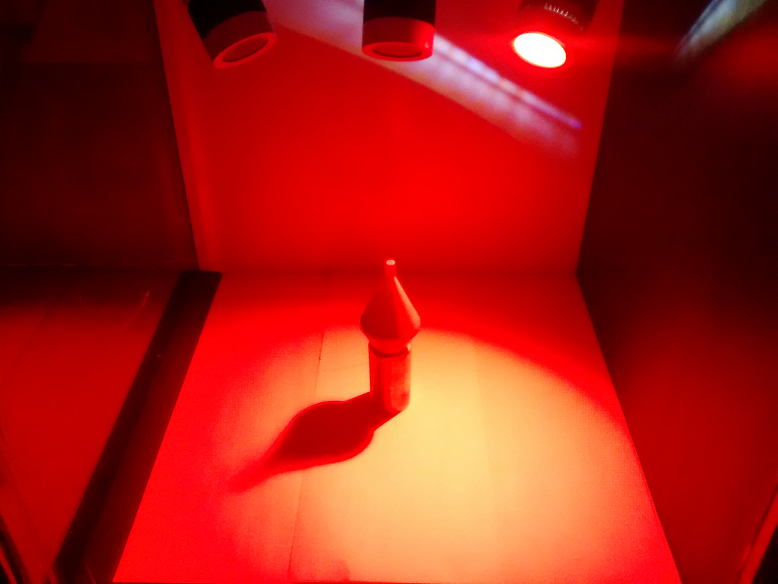
\includegraphics[width=\textwidth]{demo_1}
        \caption{A red object in red light}
        \label{img_color_demo_1}
    \end{subfigure}
    ~ %add desired spacing between images, e. g. ~, \quad, \qquad, \hfill etc. 
      %(or a blank line to force the subfigure onto a new line)
    \begin{subfigure}[b]{0.3\textwidth}
        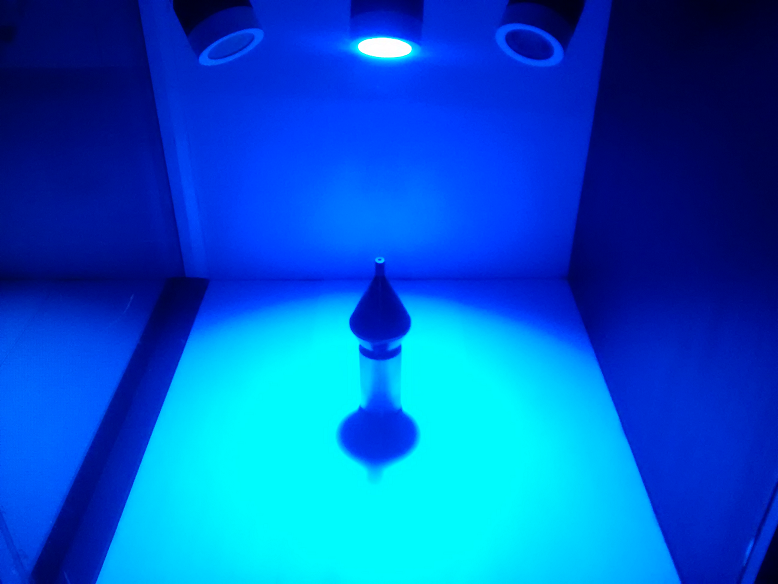
\includegraphics[width=\textwidth]{demo_2}
        \caption{A red object in blue light}
        \label{img_color_demo_2}
    \end{subfigure}
    ~ %add desired spacing between images, e. g. ~, \quad, \qquad, \hfill etc. 
    %(or a blank line to force the subfigure onto a new line)
    \begin{subfigure}[b]{0.3\textwidth}
        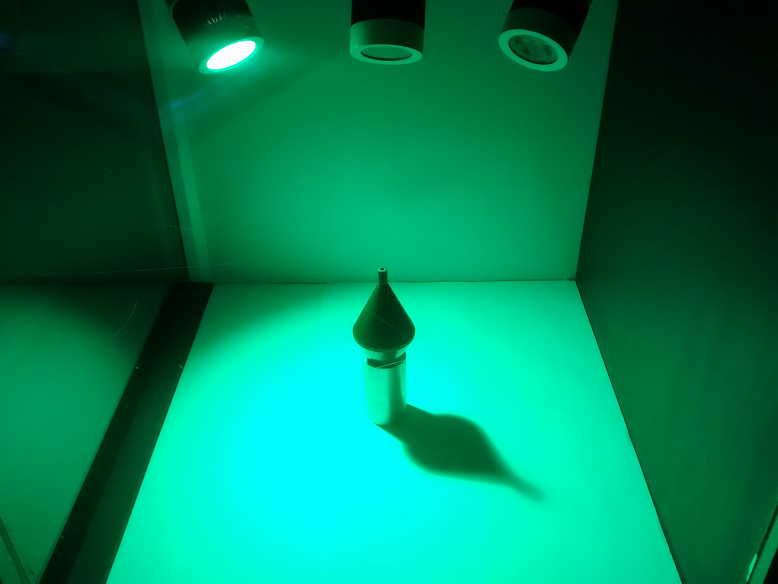
\includegraphics[width=\textwidth]{demo_3}
        \caption{A red object in green light}
        \label{img_color_demo_3}
    \end{subfigure}
    
    \begin{subfigure}[b]{0.3\textwidth}
        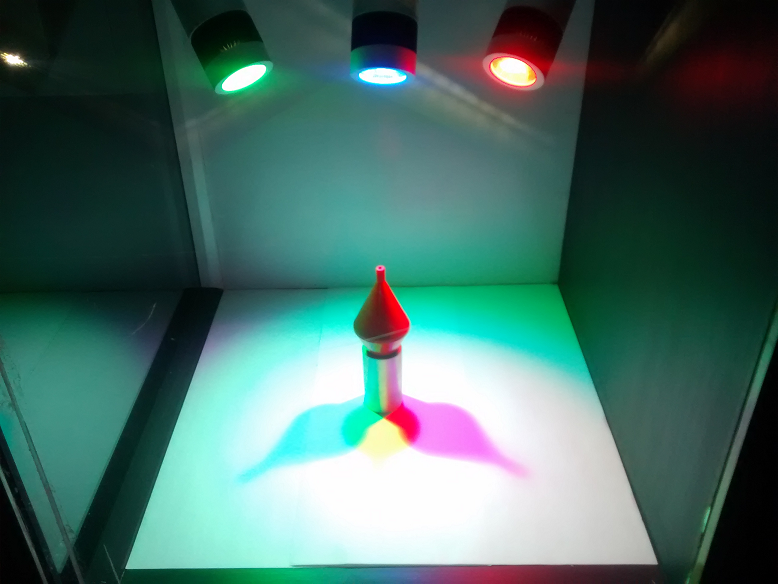
\includegraphics[width=\textwidth]{demo_4}
        \caption{The addition of colours}
        \label{img_color_demo_3}
    \end{subfigure}
    \caption{Demo on the addition of colours}\label{fig:animals}
\end{figure}

\section{The production of light}

\subsection{Thermal radiation}

Thermal radiation is the conversion of thermal energy into electromagnetic energy. But what exactly does it mean for such a transfer to occur? To understand this properly, we will of course need to understand the structure of the material that composes the matter we are providing the thermal energy to. 

Ultimately, the object producing the light is composed of constituents such as atoms and molecules arranged in some form of a lattice. You should remember from earlier courses that the \textbf{temperature} of an object is a statistical property that -- at microscopic scales -- is a reflection of the average kinetic energy of the constituents of that object. Thus, an increase in temperature would cause these atoms or molecules to start `jiggling' about more erratically (at least on an average) and would thus result in more frequent collisions between them.  

Atoms and molecules have varying behaviours when different energies are imparted to them. For example, the chemical bonds within molecules -- described by Quantum Mechanics -- vibrate at certain specific frequencies. If a collision imparts enough energy to excite one of these vibrational modes of the molecule, the kinetic energy due to the collision serves to transfer the molecule to an excited state. When it then returns back to its original state, it emits a photon having a frequency related to the energy difference between the two states. Similarly, atoms themselves have energy levels, and if a collision excites an electron to a higher level, it too returns to its ground state after emitting a photon.

The vibrational energy levels usually radiate in the infrared regime while the electronic transitions radiate in the ultraviolet. The visible region overlaps these two levels and thus obtains contributions from both. It is important to realise that since the energy is imparted through collisions, there is a continuous range of energies to which atoms and molecules may be excited and thus we get a continuous spectrum of light. However, this radiation has a very specific spectrum. It turns out that objects at the same temperature emitted more or less exactly the same spectrum of light, i.e.\ their intensities of the different wavelengths they emitted were identical. At the beginning of the last century, this was one of the `few' problems that Physics had left to address.

\subsection{Blackbody radiation and the Planck spectrum}

A black body is an idealized physical body that absorbs all incident electromagnetic radiation, regardless of frequency or angle of incidence. At thermal equilibrium (that is, at a constant temperature) it emits electromagnetic radiation called black-body radiation in the manner earlier specified. At room temperature appears it appears black, as most of the energy it radiates is infrared and cannot be perceived by the human eye. When it becomes a little hotter, it appears dull red, and as its temperature increases further it eventually becomes blue-white. The spectrum of a blackbody was known quite well experimentally, however no theoretical approach could describe the entire spectrum accurately.

At the time there were two different laws, each of which fit the experimental data in different regimes, but neither of which explained the full spectrum. For low frequencies (or long wavelengths), the law was the ``Rayleigh-Jeans law'', while for high frequencies (or short wavelengths) it was known as ``Wein's displacement law''.

\begin{figure}[!htb]
\centering
\begin{subfigure}[b]{0.45\textwidth}
        \includegraphics[width=\textwidth]{planck.png}
        \caption{Classical approximations}
        \label{planck_approx}
    \end{subfigure}
    ~ %add desired spacing between images, e. g. ~, \quad, \qquad, \hfill etc. 
      %(or a blank line to force the subfigure onto a new line)
    \begin{subfigure}[b]{0.45\textwidth}
        \hspace{0.5cm}\includegraphics[width=0.8\textwidth]{planck_temp.jpg}
        \caption{Variation with temperature}
        \label{planck_temp}
    \end{subfigure}
\caption{The Planck Spectrum for Blackbodies}
\label{planck}
\end{figure}

The problem was solved by the German physicist Max Planck who realised that `classical' physics could not be used for such blackbody radiation, and thereby ushered in Quantum Mechanics by postulating that the energies were absorbed and emitted in specific quanta. The resulting spectrum was found to be characterised by the temperature of the body and was found to fit a remarkable number of spectra from the sun to the Cosmic Microwave Background Radiation left as a remnant from the Big Bang.

\begin{tcolorbox}
\paragraph{Question: } It is often said that the Cosmic Microwave Background Radiation has a `temperature' of 2.73 K. What do you think this means?
\end{tcolorbox}

\subsection{Vapour lamps and discrete spectra}

As is only to be expected, thermal radiation is not a very efficient way of producing light. The reason for this is that the radiation emitted is not restricted to only the visible spectrum and therefore much of the light that is created cannot be used to illuminate in the general sense of the word. \textbf{Vapour lamps} such as Mercury and Sodium lamps are far more efficient, essentially because they only need enough energy to excite certain electronic spectral lines of the materials within them.

In general, vapour lamps have a low pressure noble gas (Argon in the case of a Mercury lamp and a combination of Neon and Argon for Sodium). A voltage is applied to ionise the gas by creating an electrical arc: the electrons are ripped off the atoms, introducing ions, free electrons and photons into the tube. The heat from the arc vaporises the metal inside the tube. The electrons in the metal atoms then get excited to different energy levels and they cascade down to their initial states by emitting certain special frequencies (wavelengths) of light.

\begin{figure}[!htb]
\centering
\includegraphics[width=0.75\textwidth]{hgspectrum.png}
        \caption{The mercury spectrum}
        \label{hgspectrum}
\end{figure}


\begin{tcolorbox}
\paragraph{Question: } Why do we need Quantum Mechanics to explain the spectrum you see when you look at a Mercury or Sodium vapour lamp? What would it look like if the atom were a classical object? 
\paragraph{Hint: } Consider the atom to be a `solar-system', like the Rutherford model. 

\paragraph{Question: } Can you explain the fact that you \textit{also} see a continuous spectrum on the background of the spectral lines of Sodium or Mercury when you examine their spectra?
\paragraph{Hint: } What causes a continuous spectrum?
\end{tcolorbox}

\subsection{Lasers}

Lasers are devices that emit electromagnetic radiation through a process known as \textbf{stimulated emission}. The term `Laser' itself originated as an acronym of \textit{Light Amplification by Stimulated Emission of Radiation} (which is why spelling the word with a `z' is highly incorrect). We have so far observed the production of light through a process known as \textbf{spontaneous emission} through electronic transitions within an atom. A laser differs from such sources in that it emits light \textit{coherently}, spatially and temporally. 

In the case of spontaneous emission, imagine we have two energy levels $E_0$ and $E_1$. If we manage to excite an electron in an atom to state $E_1$ , it will fall back to $E_0$ spontaneously, emitting an appropriate photon. However, both the direction and the phase of this light will be random. Furthermore, the amount of time the electron spends in this excited state (i.e.\ \textit{when} the photon is emitted) may also vary through the laws of Quantum Mechanics\footnote{Very much like the famous Heisenberg uncertainty principle $\Delta x \Delta p \geq \hbar$, there is another relation $\Delta E \Delta t \geq \hbar$ which roughly states that the time ($\Delta t$) an electron spends in state is inversely proportional to the energy difference between it and the ground state ($\Delta E$).}.

It is, however, desirable to have a coherent, monochromatic source of radiation for many different experiments (some of which you have already performed in the laboratory in these past few sessions). In order to achieve such a source, we will have to turn to another physical process known as stimulated emission.

It turns out that if we manage to excite the electron of an atom (using some sort of `pump') to the energy state $E_1$ and then \textit{pass a photon of exactly the same frequency as $\Delta E/\hbar$} near the atom, there is a very high probability that photon emitted when the $E_1 \rightarrow E_0$ transition occurs will be identical to the passing photon. In this way, we can `amplify' the original passing photon to get two photons having exactly the same phase, direction and wavelength. Such a process is known as `stimulated emission'. 

\begin{figure}[!htb]
\centering
\includegraphics[scale=0.5]{img_emission.png}
\caption{Absorption, Spontaneous Emission and Stimulated Emission}
\label{img_emission}
\end{figure}

\section{The diffraction of light}

Diffraction occurs in waves when they bend around small obstacles or when they spread out after passing through narrow apertures. The standard way of analysing such a problem is some form of `Huygen's Principle', where we define \textit{wavefronts}, each point of which is the source of \textit{secondary waves} which in turn interfere, producing the pattern that you see on the screen. The introduction of these wavefronts -- albeit highly successful -- is slightly ad-hoc and not completely justified physically. This is understandable, as Huygens did not have the right tool (total integral calculus) to describe this phenomenon mathematically. Most of the mathematics was fleshed out by another great Physicist, Augustin-Jean Fresnel. This mathematics is quite involved and as I am certain that you will be subjected to it in great detail during your course on optics, I will not attempt to explain it in too much detail. 

Suffice it to say that the presence of an obstacle of a certain length $a$ in the direction of propagation of light causes some light to shift slightly and traverse a slightly larger distance. This so-called \textit{path-difference} -- dependent on the size of the obstacle $a$ -- induces a difference in \textit{phase} which in turn leads to the light interfering after it passes around the obstacle and producing a pattern of maxima and minima on the screen. Obviously, changing $a$ we would get a different pattern and so a close inspection of the interference pattern provides us with information on the dimension of the obstacle.

\subsection{Babinet's Principle}

Babinet's principle states that

\begin{center}
\textit{Complementary objects produce the same different pattern, except for the intensity of the central maxima.}
\end{center}

We will provide a quick `proof' of this after some mathematical baggage in the subsequent sections. 

\begin{tcolorbox}
\paragraph{Question: }Two objects are complementary if one of them is transparent when the other is opaque and opaque when the other is transparent. What are the complementary objects of the following:

\begin{enumerate}
\item A narrow slit of width $d$.
\item A circular aperture of diameter $d$.
\end{enumerate}
\end{tcolorbox}

Henceforth we will not differentiate between the patterns made by such complementary objects.

\subsection{The single slit}

When the path difference due to a single slit (or thin wire) is exactly equal to an integral number of wavelengths of the light used, the waves \textit{interfere destructively}. As a result, minima occur whenever

\begin{equation*}
\underbrace{a \sin{\theta_n}}_{\text{path difference}} = \underbrace{n \lambda}_{\substack{\text{integral number} \\ \text{of wavelengths}}}
\end{equation*}

I would like to stress that the above way of interpreting mathematical equations is very important, as it attaches a physical significance to every mathematical entity in the equation.


\begin{tcolorbox}
\paragraph{Question: } What happens to $\theta_n$ when you increase $a$? 

\paragraph{Question: } Using the above equation, what is the \textbf{smallest} length you can probe using a light of wavelength $\lambda$? Prove this mathematically.

\paragraph{Question: } Is there a maximum length above which light of a wavelength $\lambda$ can no longer probe? If yes, prove it mathematically. If no, what additional constraints are introduced when probing larger length scales?
\end{tcolorbox}

Observing the pattern in Figure \ref{img_diff} you can clearly see that the intensity is not a constant, but seems to vary with angle. It turns out that -- as a function of the angle $\theta$ -- the intensity falls as 

\begin{equation*}
I(\theta) = I(0) \left( \frac{\sin{\beta}}{\beta}\right)^2 \quad \quad \text{where  } \beta = \frac{\pi a \sin \theta}{\lambda}
\end{equation*}

\begin{figure}[!htb]
\centering
    \begin{subfigure}[b]{0.45\textwidth}
        \includegraphics[width=0.8\textwidth]{fraun_theory.jpg}
     %   \caption{}
        \label{fraun_theory}
    \end{subfigure}
\begin{subfigure}[b]{0.45\textwidth}
       \includegraphics[scale=0.2]{fraun.jpg}
     %   \caption{Pattern on the screen}
        \label{fraun}
    \end{subfigure}
\caption{Diffraction pattern due to a single slit}
\label{img_diff}
\end{figure}


\begin{tcolorbox}
\paragraph{Question: } Can you sketch the above function? Write down an equation to find its zeros. Does it look familiar?
\end{tcolorbox}

\subsection{The single helix}

The single helix has, associated with it, two length scales: the thickness of the wire and the spacing between the wires (the `pitch'). The pitch works wither as two thin wires separated by a distance $P$, or alternatively a single slit of width $P$.

The entire pattern can thus be decomposed into a diffraction grating angled up at an angle $\alpha_1$, a diffraction grating angled down at an angle $\alpha_1$ (both of which have a thickness $a$), and diffraction gratings angled up (and down) at the same angle (of thickness $P$). Thus, these four objects combine together to get the $X$ shaped pattern on the screen.

\subsection{The double helix}

This pattern can be decomposed in a very similar fashion as the single helix, except that there is now another length scale associated with the object: the \textit{separation} between the two helices $d$, which produces another diffraction pattern on each arm of the $X$.



\begin{figure}[!htb]
\centering
\includegraphics[scale=0.2]{helices.png}
\caption{Schematics of a single and double helix}
\label{helix}
\end{figure}



\section{The Fourier Transform}

It turns out that the diffraction patterns and the obstacles that produce them are very closely related by an extremely cool mathematical relationship called a \textbf{Fourier Transform}. You will be studying about this in great detail in your mathematical physics courses and -- should you wish to continue in Physics --  it will be impossible for you to avoid it in the future. The Fourier Transform, as you might imagine, is quite closely related in principle to the Fourier Series you have already encountered and I will try to motivate this relationship in the subsequent sections.

\subsection{The epicycles}

As I was researching for this class I discovered something absolutely fabulous that I thought I \textit{had} to tell you. To understand this, we will have to go back to the oldest natural science: astronomy. The Greeks -- as most cultures of antiquity -- were very interested in the motions of the heavens. They were also very interested in symmetry and harmony, different ideas which found a synthesis in many of their theories of the world. 

The sphere, of course, being extremely symmetric was their orbit of choice to describe the heavens. Plato (circa 400 BC) came up with the notion of the Earth at the center of the universe and all other objects orbiting it in spherical trajectories. There were, however, certain annoying heavenly bodies that refused to behave as expected. These were called `wanderers', \textit{planétai}. The motion of these planets caused them considerable distress, as they were quite a fly in the ointment of symmetry. A solution to the problem was provided by Ptolemy.

The problem was that if you watch the planets carefully, they sometimes move backwards in the sky. So Ptolemy came up with the following idea: planets move around one big circle, but they move around a little circle at the same time. Imagine spinning a stick around you, the edge of which is attached to a rotating wheel. The planet would move like a point on the edge of the wheel; these circles were known as `epicycles'. This theory turns out to be wrong, but more importantly it is a \textit{bad} theory, for a reason that we shall soon see. It turns out that the orbit of any planet -- viewed from earth -- can be described to arbitrary accuracy by adding enough epicycles, as can be seen \href{https://www.youtube.com/watch?v=QVuU2YCwHjw}{in this amazing YouTube video}.

\begin{figure}[!htb]
\centering
\includegraphics[scale=0.4]{epicycles.png}
\caption{Epicycles and planetary motion}
\label{epicycles}
\end{figure}

The planet moves about in trajectory on a plane. Let us try to understand this mathematically. An easy way to do this in two dimensions is to superimpose a complex plane over real space and consider the motion of this particle as if it were moving about in this plane. You can easily justify this to yourself realising that circles are much easier to represent using complex numbers. The motion of a point on the edge of a single circle rotating at a frequency $\omega$ and having a radius $R$ is given by

\begin{equation*}
z(t) = R e^{i \omega t}
\end{equation*}

For two circles it would be 


\begin{equation*}
z(t) = R_1 e^{i \omega_1 t} + R_2 e^{i \omega_2 t}
\end{equation*}

We could now imagine adding three, four, or even an infinite number of circles, with every possible angular frequency. In this case, the sum would become an \textit{integral}, and the discrete indices of $R_1, R_2, ...$ etc. will be replaced by a continuous function $R(\omega)$. Thus,


\begin{equation*}
z(t) = \int^\infty_{-\infty} R(\omega) e^{i \omega t} \dd \omega
\end{equation*}

This new function $R(\omega)$ is called the Fourier Transform of $z(t)$. Giving you the function $R(\omega)$ is equivalent to giving you all the information in $z(t)$.

Let's examine what this means. It means that any arbitrary time dependent function $z(t)$ can be perfectly emulated by infinitely many circles of different frequencies all added up, provided that their radii are `correctly' weighted with respect to their frequencies (the function $R(\omega)$ we just saw). We could now add a further constraint that would simplify our analysis. Suppose now that the function is \textbf{periodic}, meaning that the path closes back on itself. Then, most frequencies  are no longer necessary, and only integral values of the frequency of the slowest circle contribute to the function. In this case, the integral reverts back to an infinite countable sum.


\begin{equation*}
z(t) = \sum_{n = -\infty}^\infty R_n e^{i n \omega_0 t}
\end{equation*}

which should look familiar. You could that the first ten or twenty and ignore the rest, fitting the data to any level of precision you wish.

\subsection{The inverse transform}

Diffraction, as I already mentioned, produces a pattern on the screen that is a Fourier Transform of the obstacle or aperture.We will use this face to ``prove'' Babinet's Principle, however we still have a little more math to get out of the way. 

We have already seen that if we use the earlier mentioned formula for the Fourier Transform\footnote{The actual definition of the Fourier Transform and its inverse are occasionally reversed, and there are also factors of $2\pi$ that appear and disappear. These, however, do not affect our strictly qualitative analysis.}, then you can also invert the operation exactly as you would in the case of Fourier series. 

\begin{tcolorbox}

\paragraph{Forward Fourier Transform}

\begin{equation*}
z(t) = \int^\infty_{-\infty} R(\omega) e^{i \omega t} \dd \omega
\end{equation*}

\paragraph{Inverse Fourier Transform}

\begin{equation*}
R(\omega) = \int^\infty_{-\infty} z(t) e^{-i \omega t} \dd t
\end{equation*}

\paragraph{Note: } Notice that the two variables $t$ and $\omega$ in question here are related inversely. This is characteristic of Fourier Transforms.

\end{tcolorbox}

\subsection{The Dirac Delta function}

The last mathematical object that we will have to deal with is the Dirac Delta function that most of you must have already heard of. It is a strange function\footnote{Later, you will learn that it is not really even a function, but rather a \textit{distribution}.}. This function is zero everywhere, except at the origin where it is infinite.

\begin{equation*}
\delta (k) = \begin{cases}
              \infty, & k = 0\\
               0,              & \text{otherwise}
             \end{cases}
\end{equation*}

It is defined by its action on other functions. In particular,

\begin{equation*}
\int_{-\infty}^\infty \delta(k) f(k) \dd k = f(0)
\end{equation*}

i.e.\ it picks up \textit{only} the value at 0.

\begin{tcolorbox}
\paragraph{Question: } What is the Fourier Transform of $\delta(k)$?

\paragraph{Question: } What do you think is the Fourier Transform of 1?
\paragraph{Answer: } It turns out to be $\delta(k)$.
\end{tcolorbox}


\subsection{Proving Babinet's Principle}

Here is a rudimentary proof of Babinet's principle. Let us begin by drawing out two complementary objects, a slit and a thin wire of the same thickness.

\begin{figure}[!htb]
\centering
\includegraphics[scale=0.5]{complementary.png}
\caption{Complementary objects: A thin wire and a narrow slit}
\label{img_complementary}
\end{figure}

Let us suppose that we add both of these objects. The resulting pattern will simply be 1, as they are complementary. This will happen to any pair of complementary objects. Thus,

\begin{equation*}
f(x) + f_\text{comp}(x) = 1
\end{equation*}

We know the following three things:

\begin{enumerate}
\item The Fourier Transform is linear (since it's an integral),
\item The Fourier Transform represents what we will see on the screen.
\item The Fourier Transform of 1 is $\delta(k)$.
\end{enumerate}

Thus, if we call $\widetilde{f}(k)$ and $\widetilde{f}_\text{comp}(k)$ the Fourier transforms of $f(x)$ and $f_\text{comp}(x)$, then taking the Fourier transforms of the last equation, we get

\begin{equation*}
\widetilde{f}(k) + \widetilde{f}_\text{comp}(k) = \delta(k)
\end{equation*}

Now this might appear to be a particularly formidable equation to solve, but we shall solve it \textit{à la physicienne}. The Dirac Delta is zero almost everywhere. In fact, it is zero everywhere \textit{except} at the origin (i.e.\ everywhere that Babinet's principle holds!) and so we shall consider every point \textit{except} the point directly in front of the beam\footnote{Remember that Babinet's principle also does not hold for the intensity of the central beam.}. Of course, in this case, $\delta(k) = 0$. Thus,

\begin{equation*}
\widetilde{f}(k) + \widetilde{f}_\text{comp}(k) = 0
\end{equation*}

or in other words,

\begin{equation*}
\widetilde{f}(k) = - \widetilde{f}_\text{comp}(k)
\end{equation*}

which, you will appreciate, is simply a mathematical formulation of Babinet's principle.

\subsection{Examples}

Here are some quick examples, convince yourselves that the mathematical description of the apertures is accurate. The function $\Theta(x)$ is known as Heaviside Step Function. It is defined as

\begin{equation*}
\Theta (x) = \begin{cases}
              0, & x < 0\\
              1, & x > 0
             \end{cases}
\end{equation*}


\begin{figure}[!htb]
\centering
\includegraphics[scale=0.4]{example_1.png}
\caption{A single slit}
\label{example_1}
\end{figure}

\begin{figure}[!htb]
\centering
\includegraphics[scale=0.4]{example_2.png}
\caption{A circular aperture}
\label{example_2}
\end{figure}


\begin{tcolorbox}
\paragraph{Remark: } $J_1(ka)$ is a special function known as a \textbf{Bessel function}. It occurs very frequently in Physics. You may think of it as a ``modified'' sine function, except that instead of at $x=n\pi$, the function has zeros at different values, specified on Figure \ref{example_3} below.

\paragraph{Question: } Can you explain the fact that for circular apertures, the values of $\bar{m}$ are not integers. Can you explain their values?
\end{tcolorbox}

\begin{figure}[!htb]
\centering
\includegraphics[scale=0.4]{example_3.png}
\caption{The Bessel function as a modified sinusoid}
\label{example_3}
\end{figure}

\newpage

\section*{References and additional reading}

\begin{enumerate}
\item \href{https://physics.info/planck/}{Blackbody Radiation - The Physics Hypertextbook}
\item \href{https://www.ifa.hawaii.edu/~barnes/ASTR110L_F05/spectralab.html}{Spectra in the Lab}
\item \href{http://hyperphysics.phy-astr.gsu.edu/hbase/quantum/atspect.html}{Atomic Spectra - Hyperphysics}
\item \href{https://pdfs.semanticscholar.org/8ccd/de212e9059a35c111704073aea2443984614.pdf}{How Rosalind Franklin Discovered the Helical Structure of DNA: Experiments in Diffraction}
\item \href{https://physics.stackexchange.com/questions/383138/diffraction-pattern-due-to-double-helix?rq=1}{Diffraction of a double helix - Physics StackExchange}
\item \href{https://betterexplained.com/articles/an-interactive-guide-to-the-fourier-transform/}{An Interactive Guide To The Fourier Transform}
\item \href{https://nipunbatra.github.io/blog/2016/FT.html}{Dummies guide to Fourier Transform} (This involves programming using Python)
\item \href{https://math.stackexchange.com/questions/1002/fourier-transform-for-dummies}{Fourier Transform for Dummies - Mathematics StackExchange}
\item \href{https://www.youtube.com/watch?v=QVuU2YCwHjw}{Ptolemy and Homer (Simpson) - YouTube}
\item \href{http://brettcvz.github.io/epicycles/}{The Epicycle Demonstrator - Drawing by Epicycles} (This site has some wacky examples, including the letter 'B')
\item \href{http://www.cchem.berkeley.edu/chem120a/extra/delta_functions.pdf}{Delta Functions}
\end{enumerate}



% \vbox{
% \textcolor{Blue}{\part{Assessment}}
% \tikz[remember picture,overlay]\node[shift={(-1,1)},opacity=0.6] at (current page.south east) {\includegraphics[width=17.5cm]{logo}};
% }

% \renewcommand{\chaptername}{Exam}

% \title{\vspace{-2cm} PHY102: Conceptual and Procedural Understanding\\\vspace{0.25cm} {Written examination}}
\author{}
\date{\vspace{-2cm} 4th May, 2018}

\maketitle

\vspace{-1.5cm}
\begin{center}
\hrulefill\\
\textbf{Instructions:}

\begin{itemize}
\item \textbf{Read the question paper carefully!}
\item The total duration of the written exam is \textbf{90 minutes}.
\item You are required to return the question paper with your answer sheet.
\item \textbf{No} electronic devices of any kind will be allowed during the examination.
\item Multiple choice questions and sketches must be marked on the question paper \textbf{clearly}.
\end{itemize}
\vspace{-0.9cm}
\hrulefill
\end{center}
\vspace{-0.9cm}
\section*{Multiple Choice Questions \hfill (5 marks)}

\begin{enumerate}
\item What is the distance between two successive divisions on the Vernier scale of a Vernier caliper of least count 0.02 mm?
\begin{enumerate}
\item 1 mm
\item 1/50 mm
\item 49/50 mm \hfill \textbf{(1 mark)}
\end{enumerate}


% \item With water, the colour red of a rainbow is observed at $42^\circ$. Supposing instead you had an acid solution (of density 1.5 g/cc). Red will now appear at:
% \begin{enumerate}
% \item An angle greater than $42^\circ$,
% \item An angle less than $42^\circ$,
% \item The same angle.\hfill \textbf{(1 mark)}
% \end{enumerate}


\item Why was a lens used in the Formation of Rainbow experiment? \hfill \textbf{(1 mark)}

\begin{enumerate}
\item To concentrate the light from the bulb onto the drop.
\item To make the light rays from the source parallel.
\item To create a point source from an extended source.
\end{enumerate}

\item You are given three laser sources which emit light of wavelengths $\lambda_1$, $\lambda_2$ and $\lambda_3$. On passing them through a fixed grating -- keeping all else constant -- the pattern of bright spots on the screen is observed as shown in Figure \ref{lambdaGratings}. Which of the following is true? \hfill \textbf{(2 marks)}

\renewcommand{\figurename}{\hspace{4cm} Figure}


\begin{figure}[!htb]\hspace{2cm}
\centering
\hspace{2cm}
\includegraphics[width=0.5\textwidth]{q10.png}%
\hfill\caption{How are the $\lambda$s related?}
\label{lambdaGratings}
\end{figure}
\vspace{-4cm}
\begin{enumerate}
\item $\lambda_1 > \lambda_2 > \lambda_3$
\item $\lambda_1 < \lambda_2 < \lambda_3$
\item $\lambda_2 < \lambda_1 < \lambda_3$
\item $\lambda_2 > \lambda_1 > \lambda_3$
\item $\lambda_2 > \lambda_3 > \lambda_1$
\end{enumerate}
\vspace{0.5cm}


\renewcommand{\figurename}{Figure}
\newpage
\item Three identical $12$ V bulbs (rated at 21W) are arranged in a circuit as indicated in Figure \ref{bulbGlow}. Which of the following is/are true? \hfill \textbf{(1 mark)}


\renewcommand{\figurename}{\hspace{5cm} Figure}
\vspace{-0.5cm}
\begin{figure}[!htb]
\hspace{4cm}
\centering
\includegraphics[width=0.25\textwidth]{q1.png}
\caption{}
\label{bulbGlow}
\end{figure}

\vspace{-5cm}

\begin{enumerate}
\item $L_1$ glows the brightest,
\item $L_2$ and $L_3$ glow equally brightly,
\item $L_2$ glows brighter than $L_3$,
\item $L_1$ and $L_2$ glow equally brightly.
\end{enumerate}

\vspace{2.5cm}
\renewcommand{\figurename}{Figure}

\section*{Short Answer Questions \hfill (10 marks)}



% \item State Babinet's principle and explain it with the help of an example, describing in detail the diffraction patterns observed.  \hfill \textbf{(1 mark)}


% \item What are the smallest and largest lengths that can be theoretically measured by diffraction using light of a wavelength 532 nm. Justify your answer. \hfill \textbf{(2 marks)}



\item Why does the intensity of light of a point source fall off as the inverse square of the distance from the source? \hfill \textbf{(2 marks)}


\item If $f'_0$ is the fundamental frequency of a massive spring with one end clamped, and $f_0$ is the fundamental frequency of the same spring with both ends clamped, explain why $f_0 = 2 f'_0$. You may use a suitable analogy if required. \hfill \textbf{(2 marks)}

% \item A single slit of width $a$ is placed in the way of a laser. The normalised intensity of the diffraction pattern is plotted against a function ($\pi a \sin\theta / \lambda$) of the angular separation $\theta$ as shown in Figure \ref{intensityPattern}. On the same figure (Figure \ref{intensityPattern}), sketch the pattern if the slit width is doubled. \hfill \textbf{(1 mark)}

% \begin{figure}[!htb]
% \centering
% \includegraphics[width=0.85\textwidth]{q8.png}
% \caption{Sketch the new pattern on the graph.}
% \label{intensityPattern}
% \end{figure}


\item Suggest a method to increase the intensity of the light falling on the drop in the Formation of Rainbow experiment, assuming that we cannot change the bulb or power supply. You have at your disposal many lenses of different sizes, focal lengths and powers. \hfill \textbf{(2 marks)}

\item Sketch the following graphs for a simple pendulum that is left from rest at a small angle $A$.

\begin{enumerate}
\item Position vs. Time
\item Velocity vs. Time 
\item Acceleration vs. Time \hfill \textbf{(2 marks)}
\end{enumerate} 

\item Roughly sketch a graph of the \textit{residence time} of the above-mentioned pendulum over a single cycle in Figure \ref{resGraph}. The residence time is defined as the amount of time ($\Delta t$) that the pendulum spends in a region of space ($\Delta x$). \hfill \textbf{(2 marks)}

\begin{figure}[!htb]
\centering
\begin{subfigure}[b]{0.5\textwidth}
\centering
\includegraphics[width=\textwidth]{q11.png}
\caption{Question 9(a)}
\end{subfigure}%
\begin{subfigure}[b]{0.5\textwidth}
\centering
\includegraphics[width=\textwidth]{q12.png}
\caption{Question 9(b)}
\end{subfigure}
\begin{subfigure}[b]{0.5\textwidth}
\centering
\includegraphics[width=\textwidth]{q13.png}
\caption{Question 9(c)}
\end{subfigure}
\end{figure}



\begin{figure}[!htb]
\centering
\includegraphics[width=0.85\textwidth]{q7.png}
\caption{Sketch a graph of residence time versus position.}
\label{resGraph}
\end{figure}

\newpage
~\\
~\\
\newpage
\section*{Long Answer Questions \hfill (15 marks)}



\item You are conducting an experiment to measure the time period of a simple pendulum using a \textbf{stopwatch}. At which point of the trajectory would you start counting the number of cycles? 

Now suppose instead that you are using a \textbf{digital sensor} to detect the pendulum's position. At which point of the pendulum's trajectory would you place such a sensor if you want to count the number of cycles?

Justify your answer in both the above cases. (\textbf{Hint:} You can use your answer from Question (9).)  \hfill \textbf{(3 marks)}


\item Why was soap solution used in the Surface Tension experiment? How much soap should one ideally use for the experiment? Justify your answer. \hfill \textbf{(3 marks)}



\item In the experiment for the Characterisation of an Incandescent Lamp, the circuit is set up as shown in Figure \ref{incandCirc} with a 12V lamp rated at 21W. However, the bulb is found to not glow. Explain why this happens.  \hfill \textbf{(3 marks)}

\begin{figure}[!htb]
\centering
\includegraphics[width=0.25\textwidth]{q2.png}
\caption{Explain why the bulb does not glow.}
\label{incandCirc}
\end{figure}


\item Design an experiment to find the resistance of a fuse (rated 500 mA). You are provided with a power supply ($0-5$V), two digital multimeters, and a resistance ladder. Make sure you mention \textbf{all} necessary details, including the settings of the multimeter, and provide a circuit diagram. \hfill \textbf{(3 marks)}



% \item The displacement of the free end of a slinky spring clamped at its upper end and oscillating vertically is given by 

% \begin{equation*}
% Y = A e^{-\left(\frac{b}{2m}\right) t}\cos{\omega t}
% \end{equation*}

% \noindent where $A$, $b$, $\omega$ and $m$ are constants and $t$ is time. Design an experiment to determine the factor $b/m$. Mention all the stages of data collection and interpretation, including the number of readings you will take and why, as well as graphs you will plot (if any). \hfill \textbf{(5 marks)}


% \item When drops are formed on a plane surface due to Surface Tension, the following relations are found to hold true:

% \begin{equation*}
% \begin{aligned}
% T &= k \cdot m \cdot g\\
% T &= C \cdot r^x \cdot d^y
% \end{aligned}
% \end{equation*}

% \noindent where $k$ and $C$ are constants, $r$ is the radius of the formed drop and $d$ the density of the solution. $x$ and $y$ are numbers. Design an experiment to find $x$. You are provided with a \textbf{glass plate}, \textbf{soap powder}, a \textbf{weighing balance} and \textbf{beakers}. You may include other objects if required.  \hfill \textbf{(3 marks)}



% \item Describe the diffraction pattern you would obtain using a Double Helix, indicating clearly which parameter of the Double Helix governs which parameter in the pattern. \hfill \textbf{(3 marks)}



\item Sketch the IV Characteristics of the circuits represented in Figure \ref{IVChar}. State the units on the axes of the graphs, as well as the rough values of voltage and current which characterise the circuit. \hfill \textbf{(3 marks)}

\begin{figure}[!htb]
\centering \hfill
\begin{subfigure}[b]{0.5\textwidth}
\centering
\includegraphics[width = 0.5\textwidth]{q3.png}
\end{subfigure}\hfill
\begin{subfigure}[b]{0.5\textwidth}
\centering
\includegraphics[width = 0.5\textwidth]{q4.png}
\end{subfigure}%
\hfill
\caption{Question 14 | Sketch the IV Characteristics}
\label{IVChar}
\end{figure}



% \begin{figure}[!htb]
% \centering
% \includegraphics[width=0.85\textwidth]{q9.png}
% \vspace{1.5cm}
% \caption{Sketch the pattern for a thin wire of thickness 1 mm.}
% \label{diffractionSlit}
% \end{figure}
\end{enumerate}

\begin{figure}[!htb]
\centering
\begin{subfigure}[b]{\textwidth}
\centering
\includegraphics[width=\textwidth]{q6.png}
\caption{Question 14(a)}
\end{subfigure}
\begin{subfigure}[b]{\textwidth}
\centering
\includegraphics[width=\textwidth]{q6.png}
\caption{Question 14(b)}
\end{subfigure}
\end{figure}

\newpage

% \vbox{
% \textcolor{Blue}{\part{Appendices}}
% \tikz[remember picture,overlay]\node[shift={(-1,1)},opacity=0.6] at (current page.south east) {\includegraphics[width=17.5cm]{logo}};
% }

% \renewcommand{\chaptername}{Appendix}

% \chapter{Writing a Lab Report}

\section{Objective}

To learn how to write a lab report. 

\section{Introduction}

Writing how to report an experiment you have done is one of the most important skills you will learn in the lab. The lab report starts from your log book, in which you make notes on the various stages of the experiment as you do it: (i) planning and designing the experiment, (ii) making observations, (iii) analysing data and doing relevant calculations, including error analysis (iv) interpreting your results in light of the theoretical background. What you write in your log book is to the lab report what the initial sketches of an artist are to the final work of art that she produces.

You will perhaps also want to remember that your lab report will be graded. Here are some things that you should keep in mind; they are what your instructor and teachings fellows will notice.

Make your lab report \textbf{clear} and \textbf{easy to follow}. A common mistake students make is to write extremely long and elaborate reports that convey very little. We are not looking for pages and pages of writing; in fact, from experience, we have seen that the best reports are usually \textbf{short}. It is your job to decide what is relevant and what isn't. (This is good training for the future.) What you decide to include should be arranged logically and have a certain flow. 

\begin{imp}
Your lab report may be written by hand, on Microsoft Word, or using \LaTeX. Of these options, we suggest you begin using \LaTeX\, as soon as possible: it makes your work look professional, and learning to use it is good practice.
\end{imp}

\textbf{Data does not lie.} Contrary to popular opinion, grades are not assigned on how close the value obtained agrees with the ``correct'' one. If you are supposed to verify a law of nature, and you end up disproving it, that's fine, provided that you say that you have disproved it. If however you could not verify it but say that you did, we can only assume that you didn't understand the experiment. If your results are completely different from established values, then you have probably measured or calculated something incorrectly. 

\begin{imp}
The lab report should contain \textbf{all} the information required for someone else to reproduce your experiment \textbf{and} its results.

\textbf{A non-standard answer with a clear path as to how you got there is worth significantly more than a standard answer that appears unjustified or out of nowhere. }
\end{imp}

The handouts contain questions about the experiment are scattered around the manual. Make sure you try to answer them as you write your report; these questions are included at critical points to check your comprehension, and the answers often provide ideas of what to include in a good report. 

\begin{imp}
Spend some time thinking about the format of your lab report. We don't expect something publishable in \textit{Physical Review Letters}, but on the other hand, we don't expect four pages of stream-of-consciousness writing either.
\end{imp}

\section{Essential Elements of a Report}

As stated above the the lab report should contain all the information needed for someone else to redo the experiment. This means that the following need to be written:

\begin{enumerate}
    \item A brief introduction to the experiment, including the aim, the approach to be followed, and a statement of the theoretical background, if needed. (In the introductory lab, enough theoretical background is generally provided, but that may not be true in later labs; in that case you may want to include some of the theory needed to understand the experiment.)
    \item The equipment used, with details. The details of the instruments don't need to be provided at the beginning but should be provided in the section where they are actually used. For example, if you are using Vernier calipers to measure the diameter of a set of balls, you need to specify the least count of the main scale and of the Vernier scale just before the table with the data on the diameters. 
    \item The procedure followed. This section should be very clear, and actually state the procedure \textit{you} followed, not what some book says you ought to have followed. 
    \item The data, clearly tabulated. As stated above, each table should be preceded by the details of the instrument used to collect the data.
    \item Error analysis, if needed.  
    \item Graphs, where needed.
    \item The result, clearly stated. 
    \item A discussion of the difficulties encountered, and any ideas that may have occurred to you for improvement of the experiment, or other related experiments that could be done.
    
\end{enumerate}

\subsubsection{Tables, Figures, and Graphs}

Tables, Figures, and Graphs (which we will come to in the next session) have a required standard of presentation, usually much higher than those you might put in your log book. If possible, have any tables and figures at the top and/or bottom of a page, and do not wrap text around figures or tables.

\begin{imp}
In general, you may use any software for data analysis. Beginners will usually prefer to use Microsoft Excel or Google Sheets. However, as you progress, it is \textbf{very strongly} advised that you use this lab to learn how to do very elementary plotting and data analysis using Python and Jupyter Notebook. We will come to this in the next session.
\end{imp}

\paragraph{Figures:} 
\begin{enumerate}
    \item The figures you will include in your lab report will usually be descriptions of the apparatus or schematic diagrams. 
    \item In general, they should be well marked and labelled and you should be able to refer to them through the report to better explain what you've done. 
    \item All figures should have a label (such as ``Figure 1:'' or ``Fig.1:'') at the start of a caption explaining what they describe. 
    \item Captions should be short and sufficiently informative so that anyone with some knowledge of the experiment will understand what it represents without having to refer to your report.
\end{enumerate}

\paragraph{Graphs:}
\begin{enumerate}
    \item Your graphs should be easy to read and clearly show all key features.
    \item Graphs are figures, and should therefore have a figure number at the start of their caption (``Fig.1:'', not ``Graph 1:'').
    \item Consider whether various results can be combined into a single graph.
    \item Here are some things your graph \textbf{must} have:
    
    \begin{enumerate}
        \item Labelled axes with units,
        \item Error bars, indicating the uncertainty with which you know the location of the point,
        \item A white background,
        \item Sensible maximum and minimum values so that most of the space is filled by the graph.
    \end{enumerate}
    
    \item Your graph \textbf{does not} need to have:
    
    \begin{enumerate}
        \item A title: all the information about the graph should be in the caption,
        \item Grid-marks or a border,
        \item Legends (unless the graph cannot be understood without one): this information would preferably also go into the caption.
    \end{enumerate}

\end{enumerate}


\paragraph{Tables:}

\begin{enumerate}
    \item Like figures, tables should be labelled and have a caption. However, they are \textbf{not} figures, but should instead be labelled ``Table 1:'', etc.
    \item All the entries, including the headings, should fit comfortably in the width or height of the columns or rows; long headings should be avoided. 
    \item The heading of each column should include the \textbf{unit} of all the readings in that column. (There is no need to write the unit next to each reading.)
    \item Include the uncertainties in every reading (after Session 3).
    \item Make sure the rows and columns are the same size throughout the table.
\end{enumerate}

\begin{imp}
While you will not encounter such situations in this laboratory, there are times when you may have an extremely large amount of data. \textbf{In such cases}, try to avoid tables of data that span many pages when the information is adequately given in a graph or by a few words of text; this is redundant and wasteful of space. 

However, during this introductory lab, we will ask you to always include both tables and graphs.
\end{imp}

\subsection{Data Interpretation}

The last step in your report is an \textbf{analysis} of your data. Usually, this is something that you can get from your graphs. Throughout this course you will be asked to plot graphs and to extract the relevant information from them. In general, this is something that is better learnt by doing rather than by reading.  Once a regression line has been found, the equation must be interpreted in terms of the context of the situation being analysed.

In general, it is good practice to plot \textbf{linear} graphs whenever possible. In certain cases, the relationships between physical quantities are linear, and this is easy: for example, if a ball is dropped from rest from some height, its \textbf{velocity} $v$ varies as

\begin{equation*}
    v = g t
\end{equation*}

Plotting $v$ against $t$ will give you a \textbf{linear} graph whose slope is the acceleration due to gravity. However, such a variation is not always guaranteed for all physical quantities. For example, the \textbf{position} $S$ of the same ball varies as

\begin{equation*}
    S = \frac{1}{2} g t^2
\end{equation*}

which is a \textit{quadratic} relationship. In some cases, you might be tempted to plot $S$ as a function of $t$ and fit a quadratic curve. In general, it is better to plot a graph between $S$ and $t^2$. These two quantities exhibit a linear relationship which is easier to fit, and whose slope gives you $g/2$.

Of course, if you released the same ball with some (downward) initial velocity $u$, then 

\begin{equation*}
    S = u t + \frac{1}{2} g t^2.
\end{equation*}

In such cases -- i.e.\ cases where the relationship between two quantities contains \textit{both} linear and parabolic terms -- a second-order (or polynomial of order two) fit is necessary. 

\begin{tip}
You will almost never, in an undergraduate laboratory, need to fit polynomials of orders higher than two. If you \textit{must} fit such a polynomial, make sure you have a very compelling reason (say, an equation predicted by some physical model) before attempting such a fit. 

Suppose -- in the example of the falling ball given above -- a higher-order polynomial is used. While this might \textit{appear} to fit data better as it goes through all the points, when \textit{more} data points are taken, the fit may not remain as ``good''. In such a case, however, a simple second-order polynomial would continue to fit the data just as well.
\end{tip}


You will sometimes have to fit different functions like exponentials, logarithms, and power-laws. The above ideas can help here as well, but we will see more on this in Session 2 (\textit{Graphing}).




Consider a quantity that obeys the following relationship:

\begin{equation*}
    y = A \ln(x) + B.
\end{equation*}

While the relationship between $y$ and $x$ is not linear, the relationship between $y$ and $\ln(x)$ is. Thus, if the graph between $y$ and $\ln(x)$ appears to be linear, then the slope and intercept would give us $A$ and $B$.


As a slightly more complicated example, consider a physical quantity $y$ that varies exponentially with another quantity $x$:\footnote{For example, in a diode, the variation of the current with small positive input voltage behaves in this manner.}

\begin{equation*}
    y = A\, e^x
\end{equation*}

In such a case, the equation can be rewritten as 

\begin{equation*}
    \ln(y) = \ln(A) + x
\end{equation*}

and so $\ln(y)$ and $x$ obey a linear relationship from which $A$ can be calculated.


\section{Conclusion}

Writing a coherent lab report is one of the most important skills that you can learn in this laboratory. The skill of communicating your results clearly and concisely is one that you will need to rely on frequently, irrespective of whether you choose to pursue a career in research or otherwise. 

A basic report should give the reader the most essential information related to the experiment you are performing, along with details of the procedures, materials, and conditions used in the experiment so that they may reproduce the experiment and its results should they so desire. A report should also include the data, tabulated in such a way that your interpretation of the data comes about almost naturally. Your may also choose to illustrate this by recasting your data using appropriate graphs, tables, or figures. The reader will also need to know how certain you are of your results, meaning that you should have a detailed section on the analysis of errors and uncertainties in your report. 

A good report is one that possesses all of these features, and is additionally a pleasure to read. This is by no means an easy task, but one that we hope that you will be able to master by the end of your undergraduate degree.



% \subsection{Uncertainties and their analysis}

% Quantifying uncertainties and errors is perhaps the most difficult (but nevertheless most important) part of an experiment. While we will not ask you to focus too much of your effort into error analysis in this introductory lab, in future labs you will be expected to spend most of your time analysing the uncertainties in your experiment. It is, however, imperative to understand that in experimental physics an ``answer'' without an associated interval of confidence is meaningless. How sure are you that if you (or somebody else) repeated the experiment again from scratch the answer would be \textit{exactly} the same? It is much more reasonable that the answer will be the same \textit{up to some range}. Consider the following everyday example: 

% Examine the assumptions that went into the derivation of your result. For
% instance, no friction, massless pulley, etc. Are these assumptions reasonable? If these
% assumptions don’t hold in the case of your experimental setup, how would it affect the
% result?

%  You should discuss the quality of your results. Do they seem to agree with your
% expectations? Be sure to explicitly show your calculations, and always include units.
% Include the uncertainties (experimental error) in all of your measured variables. The
% following question must be answered in this section: do your predicted (theoretical or
% accepted) results and your measured results agree within the limit of these
% uncertainties? Make a reasonable attempt to account for any discrepancies. For
% example, if your measured value is too small, try to identify factors that would cause this
%  An acceptable discussion of error analysis is much more that just stating
% “human and experimental error!” This says nothing and will receive no credit. If
% there was human error, the corrective action is to go back and carry out the procedure
% correctly. If there were experimental errors list them and describe how they will affect
% your experimental results

























% \section{Theory: The Simple Pendulum}

% The simple pendulum is a point mass suspended from a string of negligible mass attached to a pivot point, as shown in Figure (\ref{simple}). 

% \begin{figure}[!htb]
%     \centering
%     \includegraphics[scale=0.5]{figs/simplependulum.png}
%     \caption{The Simple Pendulum}
%     \label{simple}
% \end{figure}

% If a pendulum is set in motion so that is swings back and forth, its motion will be periodic. The time that it takes to make one complete oscillation is defined as the \textbf{time period} $T$ of the pendulum. Most of you will probably recognise the following formula for $T$: 

% \begin{equation}
%     T = 2 \pi \sqrt{\frac{l}{g}} 
%     \label{TimeP}
% \end{equation}

% where $l$ is the length of the pendulum from its fixed point, and $g$ is the acceleration due to gravity. Not so many of you, however, will realise that this is only true for \textbf{small displacements} around the equilibrium position. In general, when the pendulum is displaced from its equilibrium position, it experiences a restoring force $m g \sin\theta$. The differential equation describing its motion can be obtained from Newton's Second Law  $m\vb{a} = \vb{F}$.

% \begin{equation}
%     m l \dv[2]{\theta}{t} = - m g \sin\theta
% \end{equation}

% This is a difficult differential equation to solve. In the approximation that the angle $\theta$ is very small, we can replace $\sin\theta \approx \theta$, and we are left with the following differential equation:

% \begin{equation}
%     \dv[2]{\theta}{t} + \frac{g}{l} \theta = 0
% \end{equation}

% It is in this approximation that the simple pendulum is a \textbf{simple harmonic oscillator}, a very important model that you will not stop seeing the end of. In general, a quantity $Q$ is considered observe simple harmonic variation with respect to some parameter $t$ (not necessarily time) if it satisfies the following differential equation:

% \begin{equation*}
%     \dv[2]{Q}{t} + \omega_0^2 Q = 0
% \end{equation*}

% where $\omega_0$ is the time period of the oscillation, and is related to the time period of the oscillation through 

% \begin{equation*}
%     T = \frac{2\pi}{\omega_0}
% \end{equation*}

% Comparing, you should see that in our case, $$\omega_0 = \sqrt{\frac{g}{l}}$$ and $$T = 2\pi \sqrt{\frac{l}{g}}$$

% Thus, it should be clear that it is only when the amplitude is \textbf{small} that the time period follows this equation, since it is only then when you can approximate $\sin\theta$ with $\theta$.

% In this introductory experiment you will begin by verifying the above formula for the time period for small angles. You will then attempt to explore any variation of the time period with angle.
% \includepdf[pages=-]{Appendix_2a_Graphing_with_Python_solved.pdf}
% \includepdf[pages=-]{Appendix_2b_Linear_Regression_Code.pdf}
% \chapter{More Advanced Error Analysis}

\section{Objectives}

\begin{enumerate}
    \item To understand the concept of the random error.
    \item To study the propagation of errors from measured to derived quantities.
\end{enumerate}

\section{Introduction}

In the first chapter on errors, in the section on errors on time measurement, we found that the error on time measurement in our lab is almost certainly dominated by the reaction time of the observer. And, to determine this error, one method we suggested was to determine the time period many times and find the spread in the readings, using a measure called the standard deviation. The standard deviation is used in statistics to measure the characteristic spread of a random variable. The question then arises: What is a random variable? We will investigate this question in this chapter. 

The other matter we will address ourselves to in this chapter is that of propagation of errors. You will have noticed that in the earlier chapter on errors, we spoke at length on the errors on the observations themselves, e.g. the length $l$, or obtained by a simple operation from the observations, e.g. the time period $T$, but we said nothing about how this may affect quantity derived from these observations, e.g. the acceleration due to gravity $g$. It is clear that how certain we are of the time period and the length will affect how certain we are of $g$. In other words the errors on $l$ and $T$ will \textit{propagate} to $g$. How error propagates from observed quantities to derived quantities is the second subject of this chapter. 

\section{Random Errors}

To understand this, let us imagine trying to make a large number of tiles, by a manually operated machine. It is clear that though the tiles will be similar to each other, no two will be identical. The differences will be of various kinds, appearance, mass, edge length, etc. Since we want to look at the tiles through the eye of a physicist, let us concentrate on measurable quantities; we could choose edge length or mass; let us choose mass. 

The mass of a tile is what we call a \textit{random variable}, because the mass of one tile is different from that of another in a random manner (in spite of the template which tends of make them similar). If we want to find the characteristic mass of the tiles, we can weigh a number of them and find the average. However, what we are after is how different the tiles are from each other; so the mean won't do. What we could do, to begin with, is weigh a large number of them, and note them down. If we look carefully at the numbers, we will see that there is a spread. We see that numbers close to each other don't indicate much of a difference, and we'd like to think of them together. A powerful way to represent neighbouring readings together while highlighting the difference between distant readings is to draw a histogram. 
\subsection{Histogram}

In a histogram, we put the readings in a number of bins, i.e. we put all the readings in a certain range in the same bin, and we have a number of such bins to cover all the readings. There is no formula for the number of bins, but what we want a large-enough number of bins to see how the population differs from that in the others as we move across the readings, i.e. we want to see the pattern in the variation of the readings. 

The figure below shows a typical histogram, for --- readings of the mass of ---.

The bell-like shape of the pattern is characteristic. It is described by a famous mathematical function called the Gaussian. What we find is that whenever the variation from one reading to another is caused by a large number of factors unconnected with each other, this shape arises naturally. This is true in our example of the masses of a collection of tiles made with the same template. It is also true of the masses of group of human beings belonging to the same population, e.g. urban Punjabis. 

It is clear from the way we have arrived at the histogram that its width is determined by the spread of the readings. The mean does not contain information on this width; in fact what we are looking for is precisely how far the readings are, on the average, from the mean. If we imagine two artisans making the tiles, one a master who is able to achieve greater consistency and the other an apprentice, it ought to be clear that the histogram of the masses of the master's tiles will be narrower than that of the apprentice's tiles.

One way to characterise the spread of the masses might be to find the difference in mass between the heaviest tile and lightest tile. But there is something unsatisfactory about this because we are allowing the outliers to characterise and entire. What we would like to do is use all the readings to characterise the spread. This is done by the \textit{standard deviation} $\sigma$, which is given by the formula

\begin{equation}
    \sigma = \sqrt{\frac{\sum_{i=1}^{n} (x_i - \overline{x})^2}{n}},
\end{equation}

where $x_i$ is a reading, $\overline{x}$ is the mean, and $n$ is the number of readings.

For a Gaussian distribution of readings, i.e. a distribution the envelope of whose histogram is a Gaussian, about $68 \%$ of the readings are found between $x = \overline{x} - \sigma$ and $x = \overline{x} + \sigma$. Thus an arbitrary reading has a 68\% likelihood that an individual measurement will fall within one standard deviation $(\pm\sigma_x)$ of the mean\footnote{Keep in mind, however, the example of superluminal neutrinos we gave earlier: in that case, the error was \textit{assumed} to be random, and their precise data led them to a false positive. The true error turned out to be systematic, leading to \textit{different (and larger) error bars}!}. 


\begin{question}
    \paragraph{Question:} In the last paragraph we have gone from the fraction of readings in a certain range to a probability of an arbitrary reading's having a certain value. Go through this carefully and understand the argument.

    \paragraph{Question:} Do some research to find out what fraction of the readings are found in the range $\pm 2\sigma$ and $\pm 3 \sigma$ from the mean. 
\end{question}

When the significant source of error is considered to be random and the distribution is a Gaussian, random error associated with the reading is some factor times $\sigma$, the factor depending on how much confidence we wish to associate with our reading. If we choose $\sigma$ as our error -- this is a common choice -- the confidence associated with the reading is $68 \%$. 

\textbf{A note on statistics:} Consider two sets of measurements of the acceleration due to gravity:

\begin{table}[!htb]
\parbox{.45\linewidth}{
\centering
\begin{tabular}{cc}
\hline
\textbf{S. No.}&$\bm{g}\,\, (ms^{-2})$\\
\hline
1&$9.80\pm0.01$\\
2&$0.70\pm0.01$\\
3&$18.90\pm0.01$\\
4&$15.60\pm0.01$\\
5&$4.10\pm0.01$\\
\hline
Mean&$9.82\pm0.01$\\
\hline
\end{tabular}
\caption{Measurement of $g$ (Set 1)}
}
\hfill
\parbox{.45\linewidth}{
\centering
\begin{tabular}{cc}
\hline
\textbf{S. No.}&$\bm{g}\,\, (ms^{-2})$\\
\hline
1&$9.83\pm0.01$\\
2&$9.80\pm0.01$\\
3&$9.82\pm0.01$\\
4&$9.84\pm0.01$\\
5&$9.83\pm0.01$\\
\hline
Mean&$9.82\pm0.01$\\
\hline
\end{tabular}
\caption{Measurement of $g$ (Set 2)}
}
\end{table}

It would obviously be wrong to go simply by the mean and say that both these sets of data were equally reliable. In fact, stating the mean of the first set as the acceleration due to gravity \textbf{doesn't make sense}. 

Suppose we compared the mean of a data set to its \textit{dispersion} about the mean. If this is small, we could then say that there is some ``true'' value and that all the different values we measured occurred due to random fluctuations about this ``true'' value. Since the fluctuations are random, we could assume that they average out to zero, leaving us with a closer estimate to the ``true'' value than any individual reading.

\begin{question}
\paragraph{Question:} In above sets of data (with standard deviations of $7.6\,\,ms^{-2}$ and $0.02\,\,ms^{-2}$ respectively), does the quoted error of $\pm 0.01\,\, ms^{-2}$ make sense
\begin{enumerate}
    \item For Set 1?
    \item For Set 2?
    \item For Both?
    \item For Neither?
\end{enumerate}
Justify your answer quantitatively.
\end{question}

\begin{imp}
The two errors in the lab you will encounter that you cannot remove are \textbf{least count errors} and \textbf{random errors}. Remember to always compare them and \textbf{\textit{take the larger value}}. In Set 1 it makes no sense to say $g$ is specified to $(9.82\pm0.01)\,ms^{-2}$, since all of the values are much farther away than that!
\end{imp}

\begin{question}
\begin{enumerate}
    \item \textbf{Question:} Multiple measurements with the same instrument increases the
    \begin{enumerate}
        \item Accuracy
        \item Precision
        \item Both
    \end{enumerate}
    
    \item \textbf{Question:} Consider the following data-table~\\
    \begin{tabular}{cccccc}
    \hline
    \textbf{S. No.}&1&2&3&4&5\\
    \hline
    \textbf{Time Period} ($s$)& $1.2\pm0.1$&$1.2\pm0.1$&$1.2\pm0.1$&$1.2\pm0.1$&$1.2\pm0.1$\\
    \hline
    \end{tabular}~\\~\\
    The standard deviation is $0.0$. Would it be right to say that $T_\text{avg} = 1.2\pm 0.0$?
\end{enumerate}
\end{question}

However, keep in mind there are many cases where the mean  \textbf{does not} represent some true value\footnote{For example, even if the average number of siblings every student has is $1.574$, there is no student who has a non-integer number of siblings.}. There are also cases where the standard deviation contains physical information. Such cases are usually a result of statistical phenomena.

\begin{tip}
\begin{enumerate}
    \item In a coin-toss experiment with a large number of tosses, $\sigma$ gives you a measure of the bias of the coin.
    \item In a random walk, $\sigma$ can be a measure of the diffusion coefficient $D$.
    \item In shot-noise --  the statistical fluctuations of current due to the actual number of electrons flowing in the conductor per unit time -- $\sigma$ gives you a measure of Boltzmann's constant $k_B$.
\end{enumerate}
\end{tip}






\subsection{Reporting Errors}
\subsubsection{Significant figures}

The significant figures of a number are the digits in its representation that contribute to the precision of the number. In practice, we assume that all digits used to write a number are significant (except leading zeroes\footnote{Non-leading zeros are considered to be significant. If you write a number as 1,200, we assume there are four significant digits. If you only mean to have two or three, then it is best to use scientific notation: $1.2 \times 10^3$ or $1.20 \times 10^3$ . Leading zeros are not considered significant: 0.55 and 0.023 have just two significant figures.}).

\textbf{Results of simple calculations should not increase the number of significant digits}. Calculations transform our knowledge; they do not increase it! The rounding should be performed at the final step of a calculation to prevent rounding errors at intermediate steps from propagating through your work but \textbf{only} one or two
extra digits suffice to prevent this.

If you measure a value on a two-digit digital meter to be 1.0 and another value to be 3.0, it is incorrect to say that the ratio of these measurements is 0.3333333. The two values are not exact numbers with infinite precision. Since they each have two significant digits, the correct number to write down is 0.33\footnote{If this is an intermediate result, then 0.333 or 0.3333 are preferred, but the final result must have two significant digits.}.

\begin{imp}
\textbf{Do not write significant figures beyond the first digit of the error on the quantity}. Giving more precision than this to a value is not only irrelevant, \textit{it is misleading}.\\

If you're told you're using FAR too many digits, please do not try to use the excuse, ``That's what the computer gave me.'' \textbf{You} are in charge of presenting your results, not the computer!
\end{imp}


\subsubsection{Error propagation}

Experiments worth carrying out rarely measure only one quantity. Typically we measure two or more quantities and then `fold' them together in some equation or equations to determine some other quantity that we believe to depend on them. It is thus imperative that we understand how uncertainties in certain measured quantities `propagate' into other derived quantities.

For our analysis, let us assume that

\begin{itemize}
    \item $x$ and $y$ are measured quantities with uncertainties $\delta x$ and $\delta y$ respectively. These errors are considered to be \textbf{uncorrelated}, meaning that $\delta x$ and $\delta y$ are independent\footnote{For example, the precision of measuring the length of your simple pendulum has no effect on the precision of measuring time.}.
    
    \item $c$ is a constant known to known absolutely precisely (or with negligible uncertainty).
    
    \item $z$ is a quantity \textit{derived} from $x$ and $y$ and possessing a `propagated' uncertainty $\delta z$.
\end{itemize}

The formulae used to compute errors are usually not completely understood: a variety of different formulae are used in different cases, and the reasons \textbf{why} are usually lost on students. It turns out that there is only \textbf{one} way to add (uncorrelated) errors, which one can manipulate to get the rest:

\begin{imp}
If $z = x + y$, their (uncorrelated) errors add \textbf{in quadrature}:
\begin{equation}
    \delta z = \sqrt{\left(\delta x\right)^2+\left(\delta y\right)^2}
    \label{quadrature}
\end{equation}
\end{imp}

The reason for errors adding in quadrature is one that comes from statistics; it is essential that the errors be \textbf{independent} of each other (uncorrelated)\footnote{It also makes sense:  errors could be positive and some negative, simply adding them could conceivably give a smaller number (or even zero!). Thus, the next best thing is to add their \textit{squares}. }

Here is another motivation\footnote{This is \textbf{not} an explanation of why this is true!}: you could imagine two uncorrelated measurements to represent two axes ($x$ and $y$) that are orthogonal to each other (see Figure (\ref{fig:quadrature}). Imagine that you want to specify a point $z = (x,y)$: given that there is an uncertainty in both the coordinates $x$ and $y$, the point $z$ is uncertain \textbf{at most} by $\delta z = \sqrt{\left(\delta x\right)^2+\left(\delta y\right)^2}$.

\begin{figure}
    \centering
    \includegraphics[scale=0.5]{figs/quadrature.png}
    \caption{Two points $(x,0)$ and $(0,y)$, with uncertainties $\delta x$ and $\delta y$ respectively, can be summed to get a point $z=(x,y)$ with uncertainty $\delta z$. }
    \label{fig:quadrature}
\end{figure}

This formula can then be used to get the uncertainties of more complicated relations. For example, consider $z = xy$. In this case, the two quantities are \textbf{multiplied}, and so we can't use the above formula as is. We could, however, take the log, and get $\log{z} = \log{x} + \log{y}$. This is of the form $u = v + w$. We could then apply Equation (\ref{quadrature}), and find that $$\delta \left(\log{z}\right) = \sqrt{\left(\delta \left(\log{x}\right)\right)^2 + \left(\delta \left(\log{y}\right)\right)^2}$$

The uncertainty in $\log{z}$ can easily be related by taking the derivative\footnote{A differential is by definition the variation of function when its parameter changes by a small amount. We want to find how much $\log{z}$ changes when $z$ changes by $\delta z$. We use $\delta$ instead of $\dd$, since the variation is not truly \textit{infinitesimal}.}.

\begin{equation*}
    \dd({\log{z}}) = \frac{\dd z}{z} \quad \implies \quad \delta (\log{z}) = \frac{\delta z}{z}
\end{equation*}

Thus, 

\begin{equation}
    \frac{\delta z}{z} = \sqrt{\left(\frac{\delta x}{x}\right)^2 + \left(\frac{\delta y}{y}\right)^2}
\end{equation}

\begin{tip}
The following rules should exhaust most of the common cases that you will be exposed to in your undergraduate labs. Everything here can be generalised simply to a a \textit{set} of measurements $x_i$ with uncertainties $\delta x_i$.

\begin{enumerate}
    \item \textbf{Addition or subtraction by a constant:} If $z = c \pm x$, then 
    \begin{equation}
        \delta z = \delta x
    \end{equation}
    
    
    \item \textbf{Multiplication by a constant:} If $z = c x$, then 
    \begin{equation}
        \delta z = c\delta x
    \end{equation}
    
    \item \textbf{Addition or subtraction of two measured quantities:} If $z = x \pm y$, then 
    
    \begin{equation}
        \delta z = \sqrt{(\delta x)^2 +(\delta y)^2}
    \end{equation}
    
    \item \textbf{Multiplication or division of two measured quantities:} If $z = xy$ or $z = \frac{x}{y}$, then 
    
    \begin{equation}
        \frac{\delta z}{z} = \sqrt{\left(\frac{\delta x}{x}\right)^2 + \left(\frac{\delta y}{y} \right)^2}
        \label{relerror}
    \end{equation}
    
    \item \textbf{A measured quantity raised to a power:} If $z = x^c$, then
    
    \begin{equation}
        \frac{\delta z}{z} = c \frac{\delta x}{x}
        \label{powerror}
    \end{equation}
    
\end{enumerate}
\end{tip}

\begin{question}
\paragraph{Question:} Prove Equation (\ref{powerror}).~\\

\paragraph{Question:} If $z = x^2 = x \times x$, we get different answers if we use the Power Rule (Equation (\ref{powerror})) or the Product Rule (Equation (\ref{relerror})). Which of the two is correct? Why? ~\\

\paragraph{Question:} Calculate the uncertainty in $z$ if
\begin{enumerate}
    \item $z = \frac{1}{x}$
    \item $z = \frac{x}{1+x}$
    \item $z = \frac{x}{x+y}$
\end{enumerate}
\paragraph{Hint:} The last one is slightly hard. You will first write it as $z = \frac{1}{1 + u}$, where $u = y/x$. Then, calculate $\delta z$ in terms of $\delta u$, and only then $\delta u$ in terms of $\delta x$ and $\delta y$.
\end{question}



\end{document}